%\chapter{Simple Experiments Under Isca Framework}
\chapter{The Role of Climate Feedbacks in Polar Amplification}
\label{ch:polaramplification}

%\epigraph{\textit{"Essentially, all models are wrong, but some are useful."}\\ \textit{George Box}, 1987}{}
%\epigraphhead[70]{ \epigraph{\textit{"Essentially, all models are wrong, but some are useful."}}{\textit{George Box}, 1987 } }

\section{Introduction}

% \subsection{Isca model}

% Isca\index{Isca} is an open-source framework for the idealized modeling of global circulation of atmospheres, which provides various options for users to setup experiments for their own interests \citep{Vallis2018}. These options include dry and moist models, various convection and radiation schemes, a variety of land/sea configurations and different parameters for other planetary atmospheres. Taking the radiation scheme in Isca as an example, the choices include two gray radiation schemes (gray means that radiation in different wavelength is treated equally), which we call Frierson \citep{Frierson2006} and Byrne \& O'Gorman \citep[BOG hereafter;][]{Byrne2013}; an intermediate scheme with two infrared bands and one solar band, similar to \cite{Geen2016}; and a full radiation scheme, the multiband correlated-$k$ Rapid Radiative Transfer Model \citep[RRTM;][]{Clough2005}. In fact, the plentiful options in Isca offer users an opportunity to explore the models with different levels of complexity under the same framework.

% %\citealp{Clough2005}
% %In addition, the Isca model provides a python wrapper for the model to configure and run the experiments easily. 
% %it is to provide a means whereby a complex system may be easily modelled in different ways, with different levels of complexity, thus providing a nearly continuous pathway from comprehensive numerical modelling to conceptual modelling and theory for Earth and planetary atmospheres (Isca paper)

% However, there are no interactive cloud schemes, dynamical ocean and sophisticated land-surface models in Isca currently, compared to the comprehensive climate models. In general, clouds associated with weather and climate phenomena are the essential parts of climate system, but the simulations of clouds and their feedbacks have large uncertainties in current general circulation models (GCMs). For example, as pointed by \cite{Ceppi2017}, cloud feedback\index{cloud feedback} is the largest source of intermodel spread in equilibrium climate sensitivity in the recent Climate Model Intercomparison Project phase 5 (CMIP5). Therefore, it is very important to understand clouds and their feedback to climate systems. Generally, the models are supposed to be as close to the nature as possible for the real simulation results, which will, however, lead to the situation in which the models sometimes are too complicated to fully understand. In this case, it is of great help to employ the simple models to investigate the key mechanisms behind the various phenomena. In this chapter, we will make use of Isca to design some simple experiments investigating the zonal mean surface temperature change especially polar amplification of surface temperature change in aquaplanet simulations.%polar amplification of surface temperature change.

% %One dilemma situation for models is that they have to be as close to nature as possible to get real simulation results, which, however, results in that the models are sometimes too complicated to fully understand. 

% %In other words, the aim of my PhD project is to investigate the roles of clouds in climate system by building simple cloud schemes within Isca model. 
 
% \subsection{Polar amplification}

Polar amplification\index{Polar amplification} is the phenomenon where surface temperature in polar region rises faster than the global average \citep{IPCC2007Synth,Stocker2013}, which exists not only in observation where Arctic warming is evident \citep{Johannessen2004,Polyakov2002}, but also confirmed by models at varying levels of complexity \citep[e.g.,][]{Winton2006amplified,Langen2007,Merlis2018,Alexeev2005}.

Many discussions have focused on the sea ice and surface albedo feedback\index{Feedback!surface albedo} when discussing the mechanisms of polar amplification under global warming, as it is obvious that initial warming will melt the sea ice in Arctic region, leading to the decrease of surface albedo, which in turn will lead to the absorption of more solar radiation and cause the retreat of sea ice cover in further \citep{Serreze2011}. In fact, diminishing sea ice does play a leading role in recent Arctic temperature amplification \citep{Screen2010}. Nevertheless, polar amplification also occurs in simulations even without sea ice and surface albedo feedbacks \citep[e.g.,][]{Alexeev2005,Langen2012,Cai2005,Cai2006}. Different physical mechanisms have been proposed to explain polar amplification, including increasing northward heat transport \citep{Alexeev2005} and climate feedbacks such as Planck feedback\index{Feedback!Planck}, lapse rate feedback\index{Feedback!lapse rate}, cloud feedback and water vapor feedback\index{Feedback!water vapor} \citep{Pithan2014,Screen2010,Vavrus2004}. In addition, these mechanisms will interact with each other in the climate system, making the quantification of the contributions to polar amplification more complicated. For instance, \cite{Graversen2009} found that an increase of water vapor and total cloud cover is favorable for a stronger greenhouse effect in the Arctic than at lower latitudes with fixed albedo under doubled CO$_2$ forcing. However, \cite{Screen2010} find no evidence of changes in cloud cover contributing to recent near-surface Arctic warming.
 
\cite{Goosse2018} categorized the feedbacks in polar region into radiative and non-radiative feedbacks, in which the first linked the surface temperature change to the perturbation of top of the atmosphere (TOA) energy budget and the latter one is associated with sea ice, the ocean and other components of climate system. In fact, radiative feedback analysis can provide relative clear insights into the mechanisms of surface temperature change at high latitudes, and thus we focus on radiative feedback analysis only in this study. Besides surface albedo feedback, various feedback processes in climate system can also contribute to the polar amplification. Compared to regions with higher background temperature, a given increase in emitted radiation requires a larger temperature increase at colder regions according to Stefan-Boltzman law, indicating that Planck feedback\index{Feedback!Planck} (i.e., feedback related to uniform warming in surface and tropsphere) supports polar amplification naturally \citep{Pithan2014}.

The lapse rate feedback\index{Feedback!lapse rate}, associated with vertically non-uniform warming of atmosphere, is negative in tropical region as the vertical temperature profile is close to moist adiabatic. It is positive in polar regions due to the larger static stability, leading to 'top-heavy' and 'bottom-heavy' warming profiles in tropical and polar regions respectively \citep{Graversen2009, Pithan2014, Manabe1975, Kim2018}. As for the water vapor feedback\index{Feedback!water vapor}, the increased water vapor will amplify the greenhouse effect and cause further warming, and is bigger in tropical regions as the increase of water vapor is greater there \citep{Taylor2013, Pithan2014}. In fact, the quantification of the relative importance of these contributions is difficult. For example, \cite{Pithan2014} pointed out that temperature feedback is the largest contribution and the surface albedo feedback is the second main contributor to Arctic amplification, which is, conversely, cited as the largest contributor in some studies \citep[e.g.,][]{Manabe1975,Winton2006amplified,Hall2004}.

%About the role of cloud... \cite{Kim2018} also pointed out that.... 

In this chapter, we will revisit the polar amplification problem with a hierarchy of radiation schemes provided in Isca model \citep{Vallis2018}, in order to investigate the roles of different climate feedbacks. As introduced in \chapref{ch:methods}, the radiation scheme choices include two gray radiation schemes, Frierson \citep{Frierson2006} and Byrne \& O'Gorman \citep[BOG hereafter;][]{Byrne2013}, and the multiband correlated-$k$ Rapid Radiative Transfer Model \citep[RRTM;][]{Clough2005}. In fact, the plentiful options in Isca offer users an opportunity to explore the models with different levels of complexity under the same framework. For instance, the role of water vapor can be examined closely, as the Frierson and BOG schemes are similar except there is no water vapor feedback in the first scheme (see details in \secref{sec:wv_fb_setup}).

This chapter is structured as follows. \secref{sec:polar_amiplicaiton_setup} describes the experiment setups, lists the details and differences of the two gray radiation schemes used in the simulations. \secref{sec:method_radiative_kernel} quantifies the Planck, lapse rate and water vapor feedbacks from three radiaiton schemes in Isca through the radiative kernel method, in which the radiative kernels are derived from the offline calculation of radiation codes. In \secref{sec:polar_amiplification_results}, we investigate the roles of heat transport and various climate feedbacks in polar amplification of surface temperature change in Isca simulations. The conclusions are summarized and discussed in \secref{sec:polar_amplification_summary}.

%With these choices, we can examine some of the mechanisms such as water vapor feedback associated with the polar amplification so as to understand them in further.

\section{Experiment setup}
\label{sec:polar_amiplicaiton_setup}

\subsection{Basic setup}

The Isca model is employed for the simulations. The configuration has 25 vertical levels and is run with spectral dynamical core at T42 horizontal resolution, roughly equivalent to 2.8 degrees in latitude and longitude. The atmosphere is coupled to a slab ocean with a depth of 10m. The insolation conditions for all the experiments are perpetual equinox without seasonal change but with diurnal variations, because the perpetual equinox insolation can cause the most evident polar amplification compared to the seasonal and annual-mean insolations \citep{Kim2018}. Three radiation schemes (i.e. BOG, Frierson and RRTM schemes) are applied in our experiments to calculate the radiative transfer, as BOG and Frierson schemes are relative simple gray radiation schemes and RRTM is a widely used full radiation scheme, which can provide a good reference for the results. The sea ice formation is not enabled in the model even if the surface temperature is below the freezing point. Furthermore, the global uniform albedo is adopted in the model, and thus the surface albedo feedback is disabled. The default CO$_2$ concentration is 360 ppm. All the experiments are run for 20 years following 10 years of spinup.
%  Oceanic heat transport is prescribed with symmetric Q-flux with respect to equator. 

%The albedo ($\alpha$) used in our experiment are 0.27, 0.3, 0.33 and 0.38, where $\alpha =0.3$ is used in the control run.

\subsection{Changing forcing through varying albedos}

The general way to investigate climate sensitivity is to evaluate the degree of warming in response to a doubling of the CO$_2$ concentration in the climate system. Actually, the external forcing can be introduced into climate system through other ways such as adding a ghost forcing  arbitrarily at the TOA \citep{Hansen1997,Alexeev2005}. Given the fact that there is no sea ice in our experiments, changes of albedo will not introduce albedo feedbacks to the climate system. Instead, it provides an simple way to perturb the radiation balance at the TOA without doubling CO$_2$ concentration. Therefore, we will first examine the zonal mean surface temperature change when varying the albedo. Specifically, four albedos, $\alpha=$0.27, 0.3, 0.33 and 0.38, are selected for each radiation scheme in this study, where the $\alpha = 0.3$ is roughly the Earth's global averaged albedo and used in the control run for each radiation scheme. $\alpha=0.27$ (0.33) decreases (increases) $10\%$ from the control run value, which will cause the warming (cooling) response to the climate system. $\alpha=0.38$ increases even more than the albedo in the control run, leading to a much colder climate state. The experiments for BOG, Frierson and RRTM radiation schemes with different albedos are shown in \tabref{tab:exp_table}.

\begin{table}[ht]
	%\setlength\extrarowheight{-3pt}
	\centering
	\caption{The experiments for BOG, Frierson and RRTM radiation schemes with four different albedos, where $1\times$ indicates the CO$_2$ concentration is not doubled.} % and 2x for the $CO_2 = 720$ppm
	\vspace{0.5em}
	\renewcommand{\arraystretch}{1.3}
	\small
	%\begin{tabular}{|c|*{4}{c|}}
	\begin{threeparttable}
	%\resizebox{0.8\textwidth}{!}{
	\begin{tabular}{c|*{4}{c}}
		\toprule
		%\diagbox{Scheme}{Albedo} & 0.38 &0.33& 0.3$^*$ & 0.27 \\
		\diagbox{Scheme}{Albedo} &\makebox[3em]{0.38}&\makebox[3em]{0.33}&\makebox[3em]{0.3\tnote{*}}
		&\makebox[3em]{0.27}\\
	    \midrule
		%Byrne \& O'Gorman &  $1\times$, $2$x & $1\times$, $2$x & $1\times$, $2$x & $1\times$, $2$x \\
		Frierson & $1\times$ & $1\times$ & $1\times$ & $1\times$ \\ 
		BOG &  $1\times$ & $1\times$ & $1\times$& $1\times$ \\
		RRTM & $1\times$ & $1\times$ & $1\times$ & $1\times$ \\
		\bottomrule
	\end{tabular}%
	\begin{tablenotes}
      \setstretch{1.3}
      \item[*] indicates the control run for each radiation scheme.
     \end{tablenotes}
	\end{threeparttable}
	\label{tab:exp_table}
\end{table}

To estimate the external forcing after changing the albedos, the fixed sea surface temperature (SST) forcing method is applied in this study \citep{Hansen2005,Feldl2013,Kim2018}, which has included the adjustment throughout the atmosphere. For each radiation scheme, the radiative forcing for experiments after changing albedos ($\alpha=0.27, ~0.33$ and $0.38$) is calculated from radiation imbalance at TOA when prescribed with the monthly mean SST profiles from control experiment.

%As shown in \tabref{tab:exp_table}, the experiments are also performed for BOG radiation scheme with CO$_2$ concentration doubled to have a reference.
% \begin{figure}[ht]
% 	\centering
% 	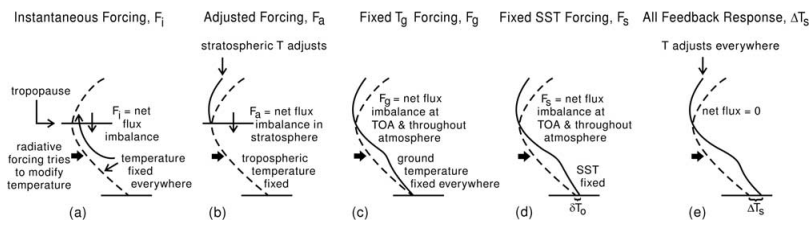
\includegraphics[width=1.0\linewidth]{{figs/polar_amp/Hansen2005_forcings}.png}
% 	\caption{ Cartoon comparing (a) $F_i$, instantaneous forcing, (b) $F_a$, adjusted forcing, which allows stratospheric temperature to adjust, (c) $F_g$, fixed $T_g$ forcing, which allows atmospheric temperature to adjust, (d) $F_s$, fixed SST forcing, which allows atmospheric temperature and land temperature to adjust, and (e) $\Delta T_s$, global surface air temperature calculated by the climate model in response to the climate forcing agent. Adapted from Figure 2 of \cite{Hansen2005}.}
% 	\label{fig:Hansen_forcing}
% \end{figure}

\subsection{Water vapor feedback in radiation scheme}
\label{sec:wv_fb_setup}
%\vspace{-1.6cm}

To examine the roles of water vapor feedback in polar amplification, the BOG and Frierson radiation schemes are employed in this study, as only one of the schemes provides moisture feedback. According to \cite{Byrne2013} and \cite{Frierson2006}, the same shortwave radiation schemes are adopted in both schemes, but the ways to calculate the longwave radiative transfer are different. Specifically, the longwave optical thickness ($\tau$) for BOG scheme in Isca is
\begin{equation}\label{eq:bog_tau}
    \frac{\text{d}\tau}{\text{d}\sigma}=a\mu+bq+c~\text{log}(\text{CO}_2/360),
\end{equation}
where $\sigma = p/p_0$, and $p_0$ is $10^3$ hPa; $q$ is the specific humidity and $\mu=1$ is a scaling parameter intended to represent absorption by well-mixed gases; $a=0.1627$, $b=1997.9$ and $c=0.17$ are values recommended in \cite{Vallis2018}. CO$_2=360$ ppm is the default CO$_2$ concentration, which has no effect on changes in longwave optical thickness at this default level. It is evident that water vapor feedback can have an impact on the optical depth in the BOG radiation scheme. However, long-wave optical depth in Frierson scheme is a function of latitude ($\theta$) and pressure ($p$) \citep{Frierson2006}, which is specified to approximate the effects of atmospheric water vapor. The surface value of optical depth ($\tau_0$) is given in the form of
\begin{equation}\label{eq:frierson_lw_optical_depth1}
\tau_0 = \tau_{0e}+(\tau_{0e}-\tau_{0p})\operatorname{sin}^2\theta,
\end{equation}
where $\tau_{0e}$ and $\tau_{0p}$ are the surface optical depth at equator and pole separately. The vertical structure of optical depth ($\tau$) is a combination of a linear term, which is included to reduce stratospheric relaxation times, and a quartic term, which is used to approximate the structure of water vapor in the atmosphere as it is an absorber with a scale height that is one quarter of the pressure scale height, and thus is given by
\begin{equation}\label{eq:frierson_lw_optical_depth2}
\tau=\tau_0\left[f_l\frac{p}{p_s}+(1-f_l)\left(\frac{p}{p_s}\right)^4\right],
\end{equation}
where $p_s$ is sea level pressure and coefficient $f_l$ is set to 0.1 in the equation. Noting that moisture is held fixed in Frierson scheme, which implies that the comparison between simulation results from BOG and Frierson schemes can demonstrate the role of water vapor feedback in polar amplification. To investigate that role in further, we re-run the experiments for BOG scheme without allowing water vapor feedback by prescribing the annual and zonal mean specific humidity profiles from the control run. In this case, the processes such as water vapor advection and convection will carry on as usual, but the moisture feedback is turned off. All the associated results will be shown in \secref{sec:polar_amiplification_results}.

%where $p_s$ is sea level pressure and the linear term ( $f_l$ is 0.1 in the equation). The quartic term is used to approximate the structure of water vapor in the atmosphere as scale height of water vapor is roughly $1/4$ of the density-scale height, but the optical thickness is fixed for each latitude and pressure level, implying that there is no moisture feedback in Frierson radiation scheme. Therefore, the comparison between simulation results from BOG and Frierson schemes could show the significance of water vapor feedback in polar amplification. To investigate the role of water vapor feedback in polar amplification in further, we re-run the experiments for BOG scheme without allowing water vapor feedback by prescribing the annual and zonal mean specific humidity profiles from the control run. Therefore, the processes such as water vapor advection and convection will carry on as usual in the BOG scheme, but the optical depth is fixed and the moisture feedback is turned off. The associated results will be shown in \secref{sec:results}.

%we write out specific humidity ($q$) from experiment where the albedo is 0.3 for BOG scheme, and then the annual and zonal mean $q$ profile will be read back into the BOG scheme for all the runs with four different albedos. 

%Write the zonally and time averaged specific humidity ($q$) into file from experiment where the albedo is 0.3.
%Read $q$ back into the BOG radiation scheme in all the runs.
%The $q$ only written into the radiation scheme not other parts of the model, which is used to fix the optical depth when altering the albedos. 
%\subsection{Roles of water vapor feedback and CO$_2$}

%%%%%%%%%%% ------------------ Section ------------ %%%%%%%%%%%%%
%\section{Method}
\section{Quantify climate feedbacks in Isca}
\label{sec:method_radiative_kernel}

\subsection{Introduction}

In order to quantify the relative importance of various contributions to polar amplification, the radiative kernel technique \citep{Soden2008,Shell2008} is used to calculate various climate feedbacks (see \secref{sec:rad_kernel_method_for_pa}). In general, climate feedback is used to characterize the response of climate system to an external radiative forcing, which can either amplify or diminish the effect of the forcings \citep{Hansen1984}. The change of net radiative flux at TOA between two different climate states, $\Delta R$, can be represented by
\begin{equation}
    \Delta R = \Delta F+\lambda \Delta T_s + \mathcal{O}\left( \Delta T_s^2 \right),
\label{eq:delta_R_relation}
\end{equation}
which can be viewed as a Taylor expansion in surface temperature change ($\Delta T_s$) \citep{Feldl2013a}. The first term, $\Delta F$, in \Eqref{eq:delta_R_relation} is the climate forcing, which is estimated by the fixed-SST method \citep{Hansen2005,Feldl2013a,Kim2018}. The second term, $\lambda \Delta T_s$, reflects the radiative flux change that is linearly depend on the surface temperature change, and $\lambda$ is the total \textit{feedback parameter}. The third term (or residual term) $ \mathcal{O}\left(\Delta T_s^2 \right)$ represents the high-order components, reflecting the non-linear interactions among different processes, which we consider to be neglected in our analysis. It should be pointed out that variables in \Eqref{eq:delta_R_relation} can be a global mean value or a function of the latitude \citep{Feldl2013a}. When neglecting the nonlinearities and interactions among the feedbacks, the feedback parameter $\lambda$ can be decomposed into the sum of different components:
\begin{equation}
\lambda=\lambda_T+\lambda_{w} +\lambda_\alpha+\lambda_C,
\label{eq:fb_decmop}
\end{equation}
where $\lambda_T$, $\lambda_{w}$, $\lambda_\alpha$ and $\lambda_C$ are the feedback parameters related to temperature, water vapor, surface albedo and cloud, respectively. In further, the temperature feedback can be divided into Planck feedback ($\lambda_P$) and lapse rate  feedback ($\lambda_L$) \citep{Soden2006}, that is $\lambda_T=\lambda_P+\lambda_L$, where the Planck feedback assumes that the tropospheric temperature change is vertically uniform and equals to the surface temperature change (in other words, there is no vertical temperature change in the troposphere) and the lapse rate feedback is associated with the vertical temperature change in troposphere that deviates from the surface temperature change \citep{Bony2006,Soden2006,Feldl2017coupled}. In our analysis, the surface albedo feedback ($\lambda_\alpha$) and cloud feedback ($\lambda_C$) are automatically neglected as there are no sea ice and cloud schemes in Isca model currently. The calculation of these feedbacks for Isca model is described in \secref{sec:rad_kernel_method_for_pa} and the analysis of the contributions to polar amplification from these feedbacks will be presented in \secref{sec:polar_amiplification_results}.

\subsection{Radiative kernel method}
\label{sec:rad_kernel_method_for_pa}

In this study, we apply radiative kernel \index{Radiative kernel} technique \citep{Soden2008,Shell2008} to calculate the climate feedbacks of Isca model. It should be mentioned that radiative kernel technique is not the only approach to quantify climate feedbacks, other methods such as partial perturbation radiative (PRP) method \citep{Wetherald1988cloud}, regression method of \cite{Gregory2004} are also used by other studies. Nevertheless, the PRP method is time consuming and the calculations have to be repeated for different simulations \citep{Shell2008}. Furthermore, the interpretation of the results must be cautious for the possible problem associated with correlated variables as pointed by \cite{Bony2006}. In contrast, the radiative kernels are calculated from the offline version radiative codes and can be used for different experiments and models. For instance, \cite{Soden2008} compare the climate feedbacks in 14 different coupled ocean-atmosphere models from the Fourth Assessment of the Intergovernmental Panel on Climate Change (IPCC AR4) with radiative kernels from three different general circulation models (GCMs) respectively, demonstrating that the strength of global feedbacks is relative insensitive to the choice of kernels.

% \begin{figure}[ht]
% 	\centering
% 	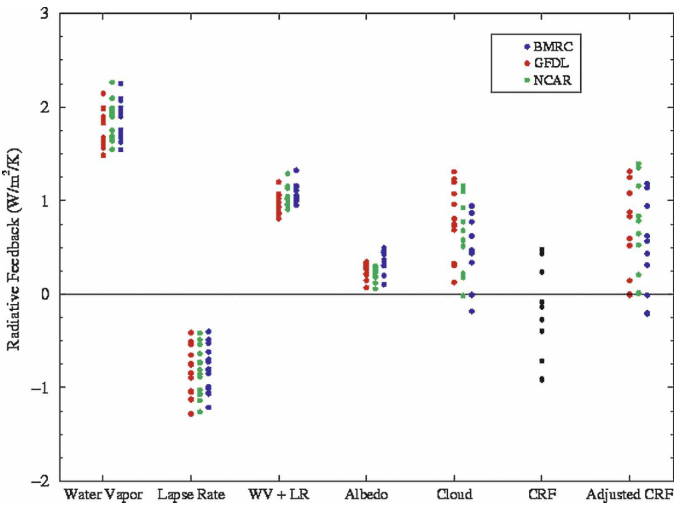
\includegraphics[width=.8\linewidth]{figs/polar_amp/fig7_Soden2008}
% 	\caption{The global-mean water vapor, lapse rate, water vapor$+$lapse rate, surface albedo, and cloud feedbacks computed for 14 coupled ocean–atmosphere models (listed in Table 1 of \cite{Soden2006}) using the GFDL (red), NCAR (green), CAWCR (blue) kernels. Adapted from the Figure 7 of \cite{Soden2008}.}
% 	\label{fig:soden2008_3_kernels}
% \end{figure}
%What's more, the radiative kernel can satisfy the goal to estimate the linearity of different climate feedbacks as the use of small differential changes is close to the "tangent linear" approximation that is the formal basis for the Taylor series expansion in Eq. (1) \citep{Feldl2013a}. 

To get the radiative kernels for one model, the model should produce high-frequency (typically either every time step or every 3 hours) output in order to get the instantaneous fields for the various variables that are needed. Initially, the model is performed with profiles without perturbation in order to get the original TOA radiation fluxes, then run with profiles where certain variable is perturbed at each level and each time step (e.g. 3 hours) to obtain the new TOA radiation fluxes corresponding to that perturbation. Specifically, the small perturbations are applied to surface temperature (+1 K), atmospheric temperature (+1 K) and specific humidity (the change amount is determined when temperature increases by 1 K but assuming relative humidity is constant) at each vertical level at each time step (e.g. 3 hours), respectively. In particular, the change of specific humidity $\Delta q$ for one layer is given by
\begin{equation}
\Delta q = q~\left(\frac{e_s(T+1)}{e_s(T)}-1\right),
\end{equation}
where $q, e_s, T$ are specific humidity, saturation pressure of water vapor and temperature respectively, and $e_s$ satisfies Clausius–Clapeyron relation\index{Clausius–Clapeyron relation}, i.e. $\frac { \mathrm { d } e _ { s } } { \mathrm { d } T } = \frac { L _ { v } e _ { s } } { R _ { v } T ^ { 2 } }$,
where $L_v$ is the specific latent heat of evaporation of water, taken to as a constant value of $2.5\times 10^6$ J kg$^{-1}$ K$^{-1}$; $R_v$, with value of $461.5$ J kg$^{-1}$ K$^{-1}$, is the gas constant of water vapor. The simple method used in this study to estimate the saturated water vapor pressure is 
%The empirical equation \citep{Alduchov1996} is used to estimate $e_s$ (units: hPa) in this study:
%\begin{equation}
%e_ s ( T ) = 6.1094 \exp \left( \frac { 17.625 T } { T + 243.04 } \right),
%\end{equation}
\begin{equation}
e_s(T) = e_{s0}\exp\left[\frac{L_v}{R_v}\left(\frac{1}{T_0}-\frac{1}{T} \right)\right],
\end{equation}
where $e_{s0}$ is a reference value of $6.1078$ hPa for this at a reference temperature $T_0=273.16$ K. After each perturbation, the changes of radiation flux at TOA are recorded and then averaged over each month to get the kernels. In fact, the traditional kernels are supposed to compute under total-sky and clear-sky conditions separately so as to obtain the radiative effect of clouds, but only clear-sky case will be calculated for Isac model at present due to the lack of cloud schemes.

%\vspace{-0.3cm}
If $\Delta R$ represents the TOA radiation flux change due to the perturbation of variable $x$, then the radiative kernel for each level is defined as $K^i_x = \partial R / \partial x_i$, which is a function of space and time. In general, the resulting kernels are weighted relative to 100-hPa thick layer in order to make it easier to compare with other different kernels, that is $\mathbb{K}^i_x = K^i_x / \Delta p_i \times 100\text{ hPa}$, where $\Delta p_i$ is the thickness of layer $i$ in units of hPa. The total radiation flux change at TOA due to $x$ perturbation is obtained by integrating from the surface to the tropopause, that is
\begin{equation}
\Delta R=\sum_{i=1}^{nlev} \frac{\partial R}{\partial x_i}{\Delta x_i},
\label{eq:delta_R_sum}
\end{equation}
where $nlev$ denotes the number of vertical levels. The tropopause height is determined following the approach developed by \cite{Soden2006}, which defines the tropopause ($H$) at $100$ hPa at the equator and $300$ hPa at the poles and varies by cosine of latitude ($\phi$) in between, that is $H=300-200 \cos\phi$. After getting the radiation response, the climate feedback parameter is defined as

%\begin{equation}
%    \Delta R=\sum_{i=1}^{n} \frac{\partial R}{\partial x_i}{\Delta x_i},
%\end{equation}
%The cliamte feedback parameters are the product of the radiative kernel for relevant variable $x$ and the climate change anomaly normilized by the local surface temperature change
\begin{equation}
%\lambda = \frac{\Delta R}{\Delta T_s} = \sum_{i=1}^{n} \frac{\partial R}{\partial x_i}\frac{\Delta x_i}{\Delta 
\lambda = \frac{\Delta R}{\Delta T_s} = \frac{1}{\Delta T_s} \sum_{i=1}^{n} \frac{\partial R}{\partial x_i}\Delta x_i,
\label{eq:lambda_def}
\end{equation}
where $\Delta T_s$ is the surface temperature change and the units of $\lambda$ is Watt per meter squared per Kelvin (Wm$^{-2}$ K$^{-1}$).
% $\lambda$ can also be depicted in $K$ or $\mathbb{K}$, that is
%\begin{subequations}\label{eq:lambda_def_K}
%	\begin{equation}
%	%\lambda = \sum_{i=1}^{nlev} K^i \frac{\Delta x_i}{\Delta T_s},
%	\lambda =\frac{1}{\Delta T_s} \sum_{i=1}^{nlev} K^i \Delta x_i ,
%	\label{eq:lambda_def_K1}
%	\end{equation} 
%	\begin{equation}
%	% \lambda = \sum_{i=1}^{nlev} \frac{\Delta p_i}{100}\mathbb{K}^i  \frac{\Delta x_i}{\Delta T_s},
%	\lambda =\frac{1}{\Delta T_s}  \sum_{i=1}^{nlev} \frac{\Delta p_i}{100}\mathbb{K}^i  \Delta x_i,
%	\label{eq:lambda_def_K2}
%	\end{equation}
%\end{subequations}
%where $\Delta p_i$ is in units of hPa.
Noting that zonal-mean variables, not the global-mean values, will be applied in \Eqref{eq:lambda_def} so we can analyze local or regional feedback, as it offers some advantages such as spatial pattern of changes \citep{Feldl2013,Feldl2017}.

In calculation of different climate feedbacks, different variables ($x$) will be employed in \Eqref{eq:lambda_def}. As for Planck feedback, the temperature change is vertically uniform in atmosphere, meaning that the air temperature change equals to the surface temperature change, so we have $x=T_s$ in \Eqref{eq:lambda_def}. Similarly, the lapse rate feedback is associated with the warming/cooling that deviates from surface temperature change, indicating that $x=T_a-T_s$ ($T_a$ denotes the atmospheric temperature) is utilized in \Eqref{eq:lambda_def}.
%Therefore, the Planck and lapse rate feedbacks can be rewritten as
% indicating that $\Delta x$ should be an array that have same size as atmospheric temperature but all the values are $\Delta T_s$.  , suggesting that $\Delta x$  has same size as atmospheric temperature but all of the values are $\Delta T_a-\Delta T_s$. 
%\begin{equation}
%\lambda_P = \frac{1}{\Delta T_s} \left( K_{T_s}\Delta T_s +\sum_i^{nlev} K_T^i \Delta T_s \right)%  = K_{T_s}+\sum_i^{nlev}K_T^i,
%\label{eq:fb_planck}
%\end{equation}
%and
%\begin{equation}
%\lambda_L =  \frac{1} {\Delta T_s} \sum_i^{nlev} K_T^i \left( \Delta T_{a}^i-\Delta T_s \right),
%\label{eq:fb_lapserate}
%\end{equation}
%respectively.
Regarding to the water vapor feedbacks, the natural logarithm of atmospheric specific humidity (i.e. $x=\ln q$) is applied in \Eqref{eq:lambda_def}, since the absorption of radiation by water vapor is approximately proportional to the natural logarithm of water vapor content \citep{Shell2008,Feldl2016,Liu2018}. %However, we find that different equations are used to calculate water vapor feedback with kernel method. For example, \cite{Feldl2016} used the following equation to calculate the water vapor feedback:
%\begin{equation}
%\lambda_w = \sum_i^{nlev} K^i_q\frac{\Delta \ln q_i}{\delta \ln (q_{s}^i)}\frac{1}{\Delta T_s},
%\label{eq:wv_fb_feldl_eq}
%\end{equation}
%where $q_s$ is the saturated specific humidity. 
Similarly, \cite{Huang2017} employ another way to calculate the water vapor feedback:

\begin{equation}
% \lambda_w = \sum_i^{nlev} K^i_q ~\frac{\Delta \ln q_i}{(\delta e_s/ \delta T)_i} \frac{1}{\Delta T_s},
\lambda_w = \sum_i^{nlev} K^i_q ~\frac{\Delta \ln q_i}{(\delta \ln e_s/ \delta T)_i} \frac{1}{\Delta T_s},
\label{eq:fb_wv_YHuang}
\end{equation}
%and $(\delta e_s/ \delta T)_i$ is estimated by $\left(e_s(T_i+1)-e_s(T_i)\right)/ e_s(T_i)$, which is similar to the method that \cite{Pendergrass2018} used to calculate the water vapor kernel (refer to the scripts on \href{https://github.com/apendergrass/cam5-kernels}{https://github.com/apendergrass/cam5-kernels}), and hence we use \Eqref{eq:fb_wv_YHuang} to calculate the water vapor kernel in this study.
and $(\delta \ln e_s)_i$ is estimated by $\left(e_s(T_i+1)-e_s(T_i)\right)/ e_s(T_i)$, which is similar to the method that \cite{Pendergrass2018} used to calculate the water vapor kernel, and hence we use \Eqref{eq:fb_wv_YHuang} to calculate the water vapor kernel in this study.
%(refer to the scripts on https://github.com/apendergrass/cam5-kernels)

% ------------------- sub SECTION ------------------- %
\subsection{Radiative kernels in Isca}
 
To calculate the radiative kernels for Isca \index{Radiative kernel!of Isca}, a 10-year control experiment ($\alpha= 0.3$) is re-run for each radiation scheme to get corresponding model outputs (e.g. temperature, specific humidity) at 3-hour frequency. Then 1-year climatology computed from the last 5-year period is taken as the basic profiles for the offline radiation codes. Then the perturbation procedure will be carried out for different variables such as surface temperature, temperature and specific humidity to obtain the surface temperature, temperature and water vapor kernels respectively. The radiative kernel results for each radiation scheme are shown below and the data sets are available at Zenodo (\url{http://doi.org/10.5281/zenodo.4282681}).

\subsubsection{Frierson and BOG scheme}

\begin{figure}[ht]
	\centering
	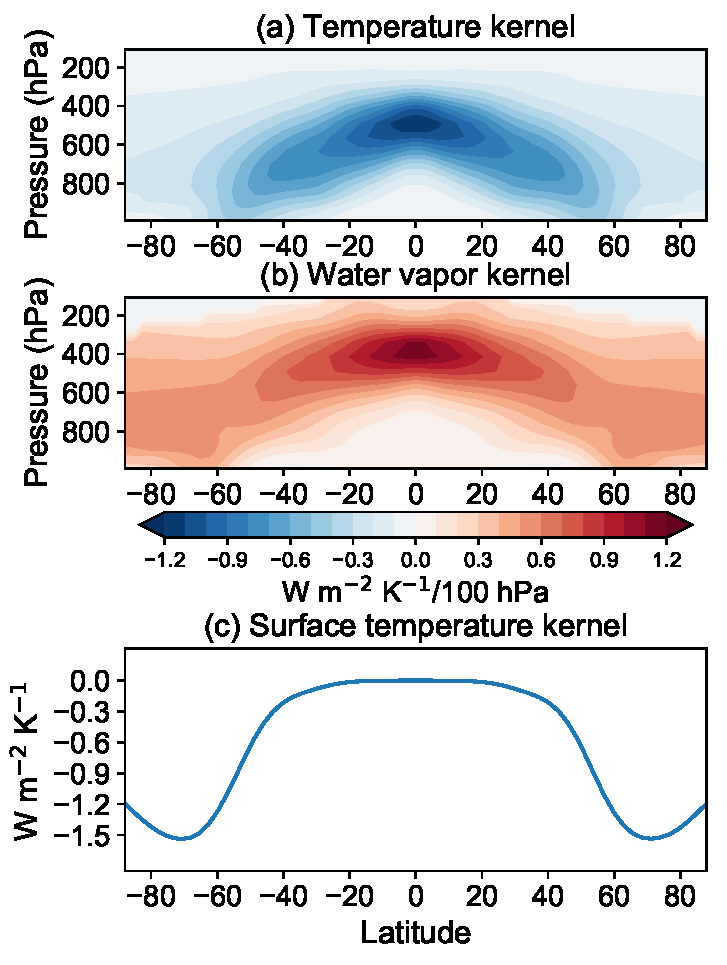
\includegraphics[width=0.45\linewidth]{figs/polar_amp/kernels_byrne}
	\caption[Annual-mean and zonal-mean temperature, water vapor and surface temperature radiative kernels for BOG radiation scheme]{Annual-mean and zonal-mean radiative kernel for the Byrne and O'Gorman (BOG) radiation scheme: (a) temperature kernel with respect to 1-K increase in atmospheric temperature, (b) water vapor kernel for a specific humidity perturbation corresponding to a 1-K temperature increase with relative humidity unchanged, (c) surface temperature kernel for 1-K perturbation in surface temperature.}
	\label{fig:bog_kernels}
\end{figure}

% \begin{figure}[ht]
%   \begin{minipage}[c]{0.6\textwidth}
%     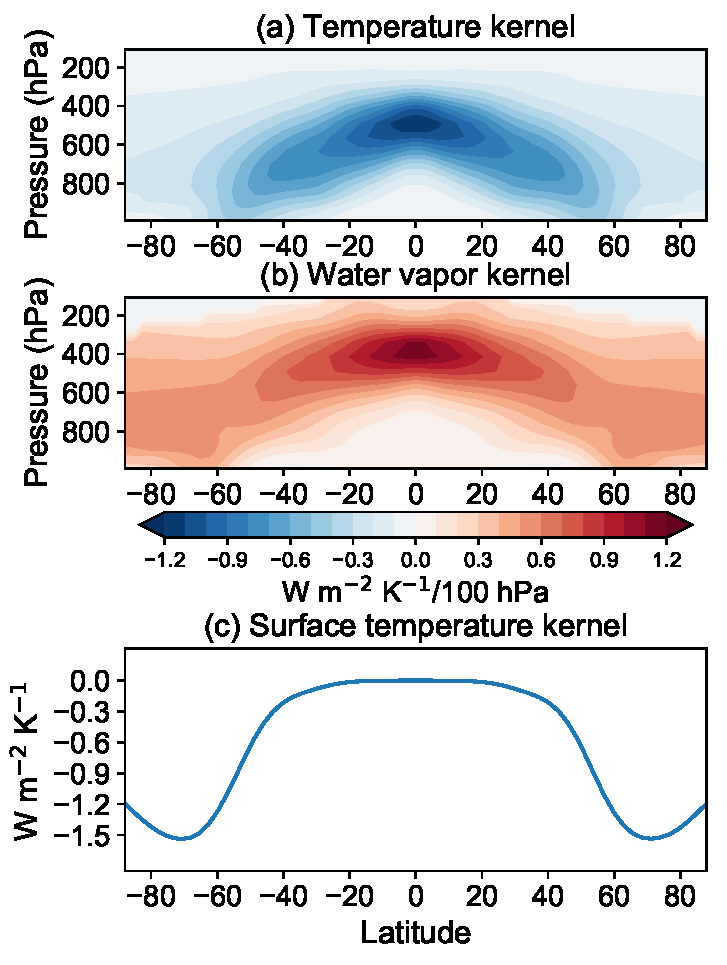
\includegraphics[width=\linewidth]{figs/polar_amp/kernels_byrne}
%   \end{minipage}
%   \hfill
%   \begin{minipage}[c]{0.35\textwidth}
%     \caption[Annual-mean and zonal-mean temperature, water vapor and surface temperature radiative kernels for BOG radiation scheme]{Annual-mean and zonal-mean radiative kernel for the Byrne and O'Gorman (BOG) radiation scheme: (a) temperature kernel with respect to 1-K increase in atmospheric temperature, (b) water vapor kernel for a specific humidity perturbation corresponding to a 1-K temperature increase with relative humidity unchanged, (c) surface temperature kernel for 1-K perturbation in surface temperature.}
%     \label{fig:bog_kernels}
%   \end{minipage}
% \end{figure}

\begin{figure}[ht]
	\centering
	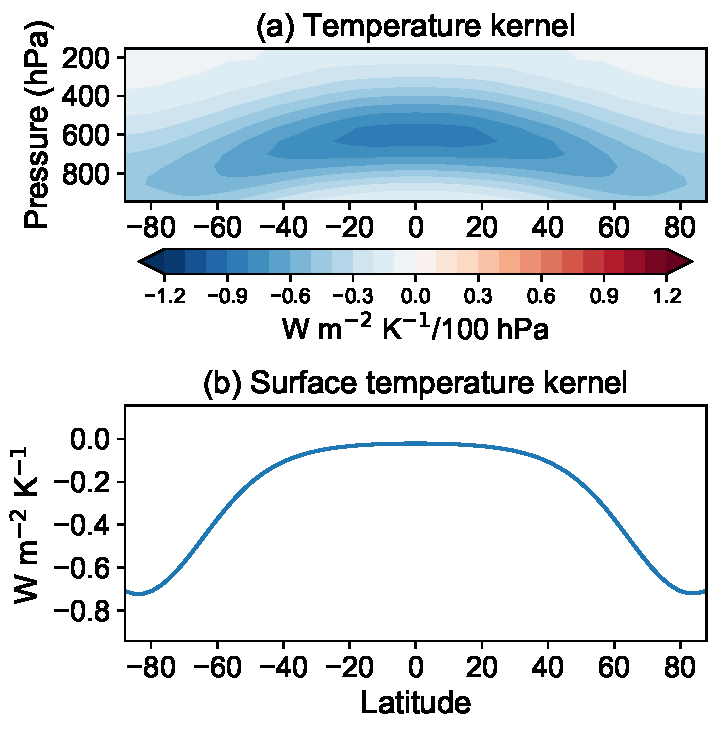
\includegraphics[width=0.45\linewidth]{figs/polar_amp/kernels_frierson}
	\caption[Annual-mean and zonal-mean temperature and surface temperature radiative kernels for Frierson radiation scheme]{As in \figref{fig:bog_kernels}, but only for temperature and surface temperature kernels in Frierson radiation scheme.}
	\label{fig:frierson_kernels}
\end{figure}

%The shortwave radiation components for Frierson and BOG schemes are the same, where the insolation varies in diurnal cycle in the simulations. The only difference between these two gray radiation schemes lies in whether there is moisture feedback in longwave parts. Specifically, in Frierson scheme, the optical thickness $\tau$ for longwave is defined as
%\begin{equation}
%\tau = \tau_{0}\left[f_{\text{l}}\left(\frac{p}{p_{\text{s}}}\right)+\left(1-f_{\text{l}}\right)\left(\frac{p}{p_{\text{s}}}\right)^{4}\right], \label{eq:frierson_optd}
%\end{equation}
%where $\tau_0$ is the optical depth at the surface, which is a function of latitude, $p_s$ and $p$ are pressure of surface and other vertical levels and $f_l$ is the coefficient to weight the linear and quartic terms, which is $0.1$ in Isca. The quartic term approximates the structure of water vapor in atmosphere. The small linear term is included to reduce the stratospheric relaxation time. It is clear that the optical depth is specified in Frierson scheme and won't change with the contents of water vapor in the model. However, the optical thickness in BOG scheme vary with specific humidity $q$, as shown in the equation of $\tau$:
%\begin{equation}
%\frac{\text{d}\tau}{\text{d}\sigma}=a{\mu}+b{q}+c~\text{log}(CO_2/360),
%\label{eq:bog_optd}
%\end{equation}
%where $\sigma = p/p_0$, $\mu=1$ is a scaling parameter intended to represent absorption by well-mixed gases and $a$, $b$, $c$ are coefficients for different terms and the suggested values are $a = 0.1627, b = 1997.9$ and $c = 0.17$. 
%Shortwave parts introduce the zenith angles in the insolation...

The radiative kernels for temperature, water vapor and surface temperature in BOG schemes are shown in \figref{fig:bog_kernels}. There is no water vapor kernel in Frierson scheme (\figref{fig:frierson_kernels}). The temperature kernel illustrates the contribution of different latitudes and levels to the change of TOA longwave fluxes. The numerical values are generally negative, indicating that an increase in temperature increases the outgoing longwave radiation (negative feedback). As shown in \figref{fig:bog_kernels}a and \figref{fig:frierson_kernels}a, the values of temperature kernels are more negative in tropical atmosphere owing to the larger sensitivity according to the Stefan-Boltzmann law, but the location of largest sensitivity is somewhat different from the temperature kernel in RRTM scheme (\figref{fig:rrtm_kernels}a), where the largest sensitivity appears near the surface in tropical regions. Low sensitivity occur near the tropopause and polar region in BOG's and Frierson's temperature kernel, reflecting the regional differences in lapse rate and emissivity \citep{Soden2008}. The vertically integrated global, annual mean of temperature kernel for BOG and Frierson radiation schemes are -3.45 and -3.65 W m$^{-2}$ K$^{-1}$ respectively, which are similar to clear-sky temperature kernel for Geophysical Fluid Dynamics Laboratory (GFDL) atmospheric model (version AM2p12b), which is 3.6 W m$^{-2}$ K$^{-1}$ estimated by \cite{Soden2008}.

The water vapor kernel for BOG scheme (\figref{fig:bog_kernels}b) demonstrates the relative importance of different level and latitudes to the strength of longwave water vapor feedback when temperature increases uniformly but the relative humidity keeps unchanged. In contrast, the values for water vapor feedback are positive almost everywhere, as the increase in the content of water vapor in atmosphere can help to increase the net incoming longwave radiation at TOA. Clearly, the water vapor kernel is largest in the deep tropics and decreases in poleward direction. The vertically integrated global and annual mean for water vapor kernel in BOG scheme is 3.61 W m$^{-2}$ K$^{-1}$, which is more than twice of clear-sky water vapor kernel (1.62 W m$^{-2}$ K$^{-1}$) of GFDL AM2p12b \citep{Soden2008}, suggesting that the water vapor feedback is much stronger in the BOG scheme.

The surface temperature kernel also contributes partially to the temperature feedback (the Planck feedback), and the warming of surface temperature increase the outgoing longwave radiation, so the surface temperature kernel are negative in all the latitudes as displayed in \figref{fig:bog_kernels}c and \figref{fig:frierson_kernels}b. But the scales of surface temperature kernel in BOG and Frierson radiation schemes are different, and the possible reason for that is the surface temperature came from their own control runs rather than the same ones.

\begin{figure}[ht]
	\centering
	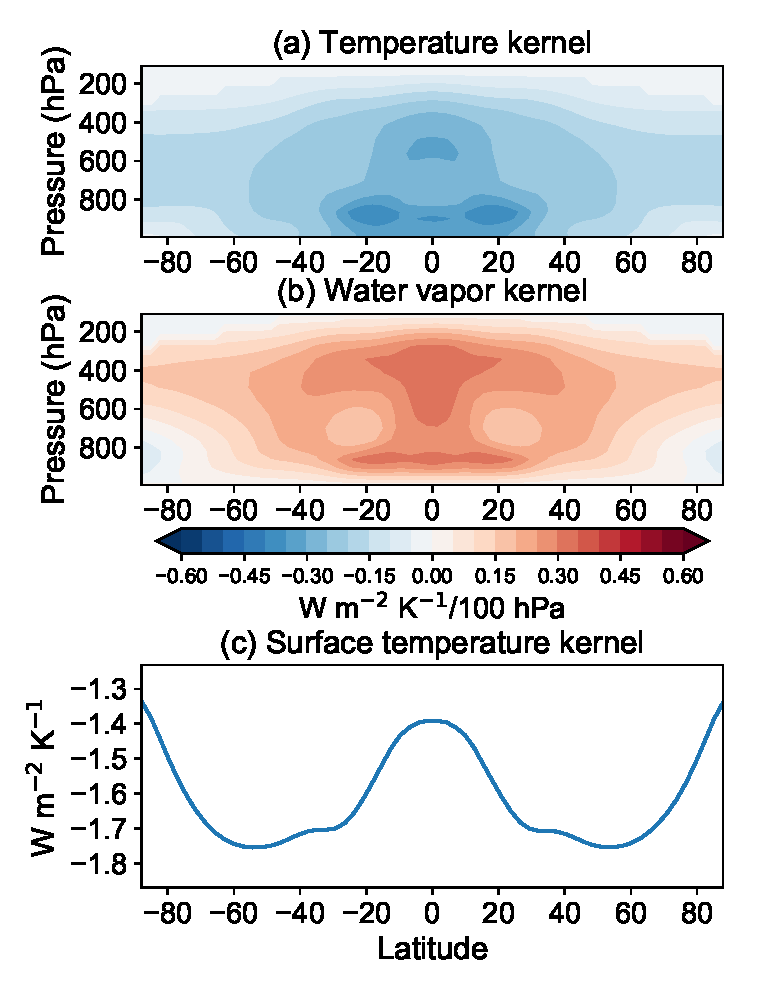
\includegraphics[width=0.45\linewidth]{figs/polar_amp/kernels_rrtm}
	\caption[Annual-mean and zonal-mean temperature, water vapor and surface temperature radiative kernels for RRTM radiation scheme]{As in \figref{fig:bog_kernels}, but for the RRTM radiation scheme.}
	\label{fig:rrtm_kernels}
\end{figure}

\subsubsection{RRTM scheme} The offline version of RRTM code is from \textit{pyrrtm} (https://github.com/tomflannaghan /pyrrtm), which provides a user-friendly python wrapper for the single-column version of RRTM scheme. The input profiles for \textit{pyrrtm} are from the Isca outputs in which the albedo is 0.3. Nevertheless, one frustrating fact is that the single-column version of RRTM will consume too much time if we perturb each level and each position every 3 hours. In order to get over this drawback, we employ zonal-mean and monthly mean profiles as the input for the \textit{pyrrtm} to calculate the radiative kernels. As shown in \figref{fig:rrtm_kernels}a, the temperature kernel for RRTM is weaker compared to the results of GFDL AM2.1 \citep[see their Fig. A1 of][]{Feldl2017coupled}, and the vertical integration of global and annual mean result is -1.79 W m$^{-2}$ K$^{-1}$, which is almost a half of the clear-sky results (-3.6 W m$^{-2}$ K$^{-1}$) of GFDL AM2p12b \citep{Soden2008}, suggesting that the feedbacks depending on this kernel would be small than other GCM's. However, the RRTM surface temperature kernel makes the situation different. It has the similar shape but the strength is much stronger compared to the surface temperature kernel of GFDL AM2.1 \citep[see their Fig. A1 of][]{Feldl2017coupled}, making the Planck feedback for RRTM comparable (\figref{fig:all_feedbacks}c). With respect to water vapor kernel for RRTM, the vertical integration of global and annual mean value is 1.65 W m$^{-2}$ K$^{-1}$, which is close to the longwave water vapor kernel results (1.62 W m$^{-2}$ K$^{-1}$) of GFDL AM2p12b, meaning that the water vapor kernel is similar to other models. Although the positive values dominate the water vapor kernels, some negative values appear in polar region, as there are temperature inversions near the surface at high latitudes, which will decrease, rather than increase, the net longwave flux in response an increase of water vapor \citep{Soden2008}. However, this does not occur in water vapor kernel for BOG radiation scheme (\figref{fig:bog_kernels}b).

% \begin{figure}[ht]
% 	\centering
% 	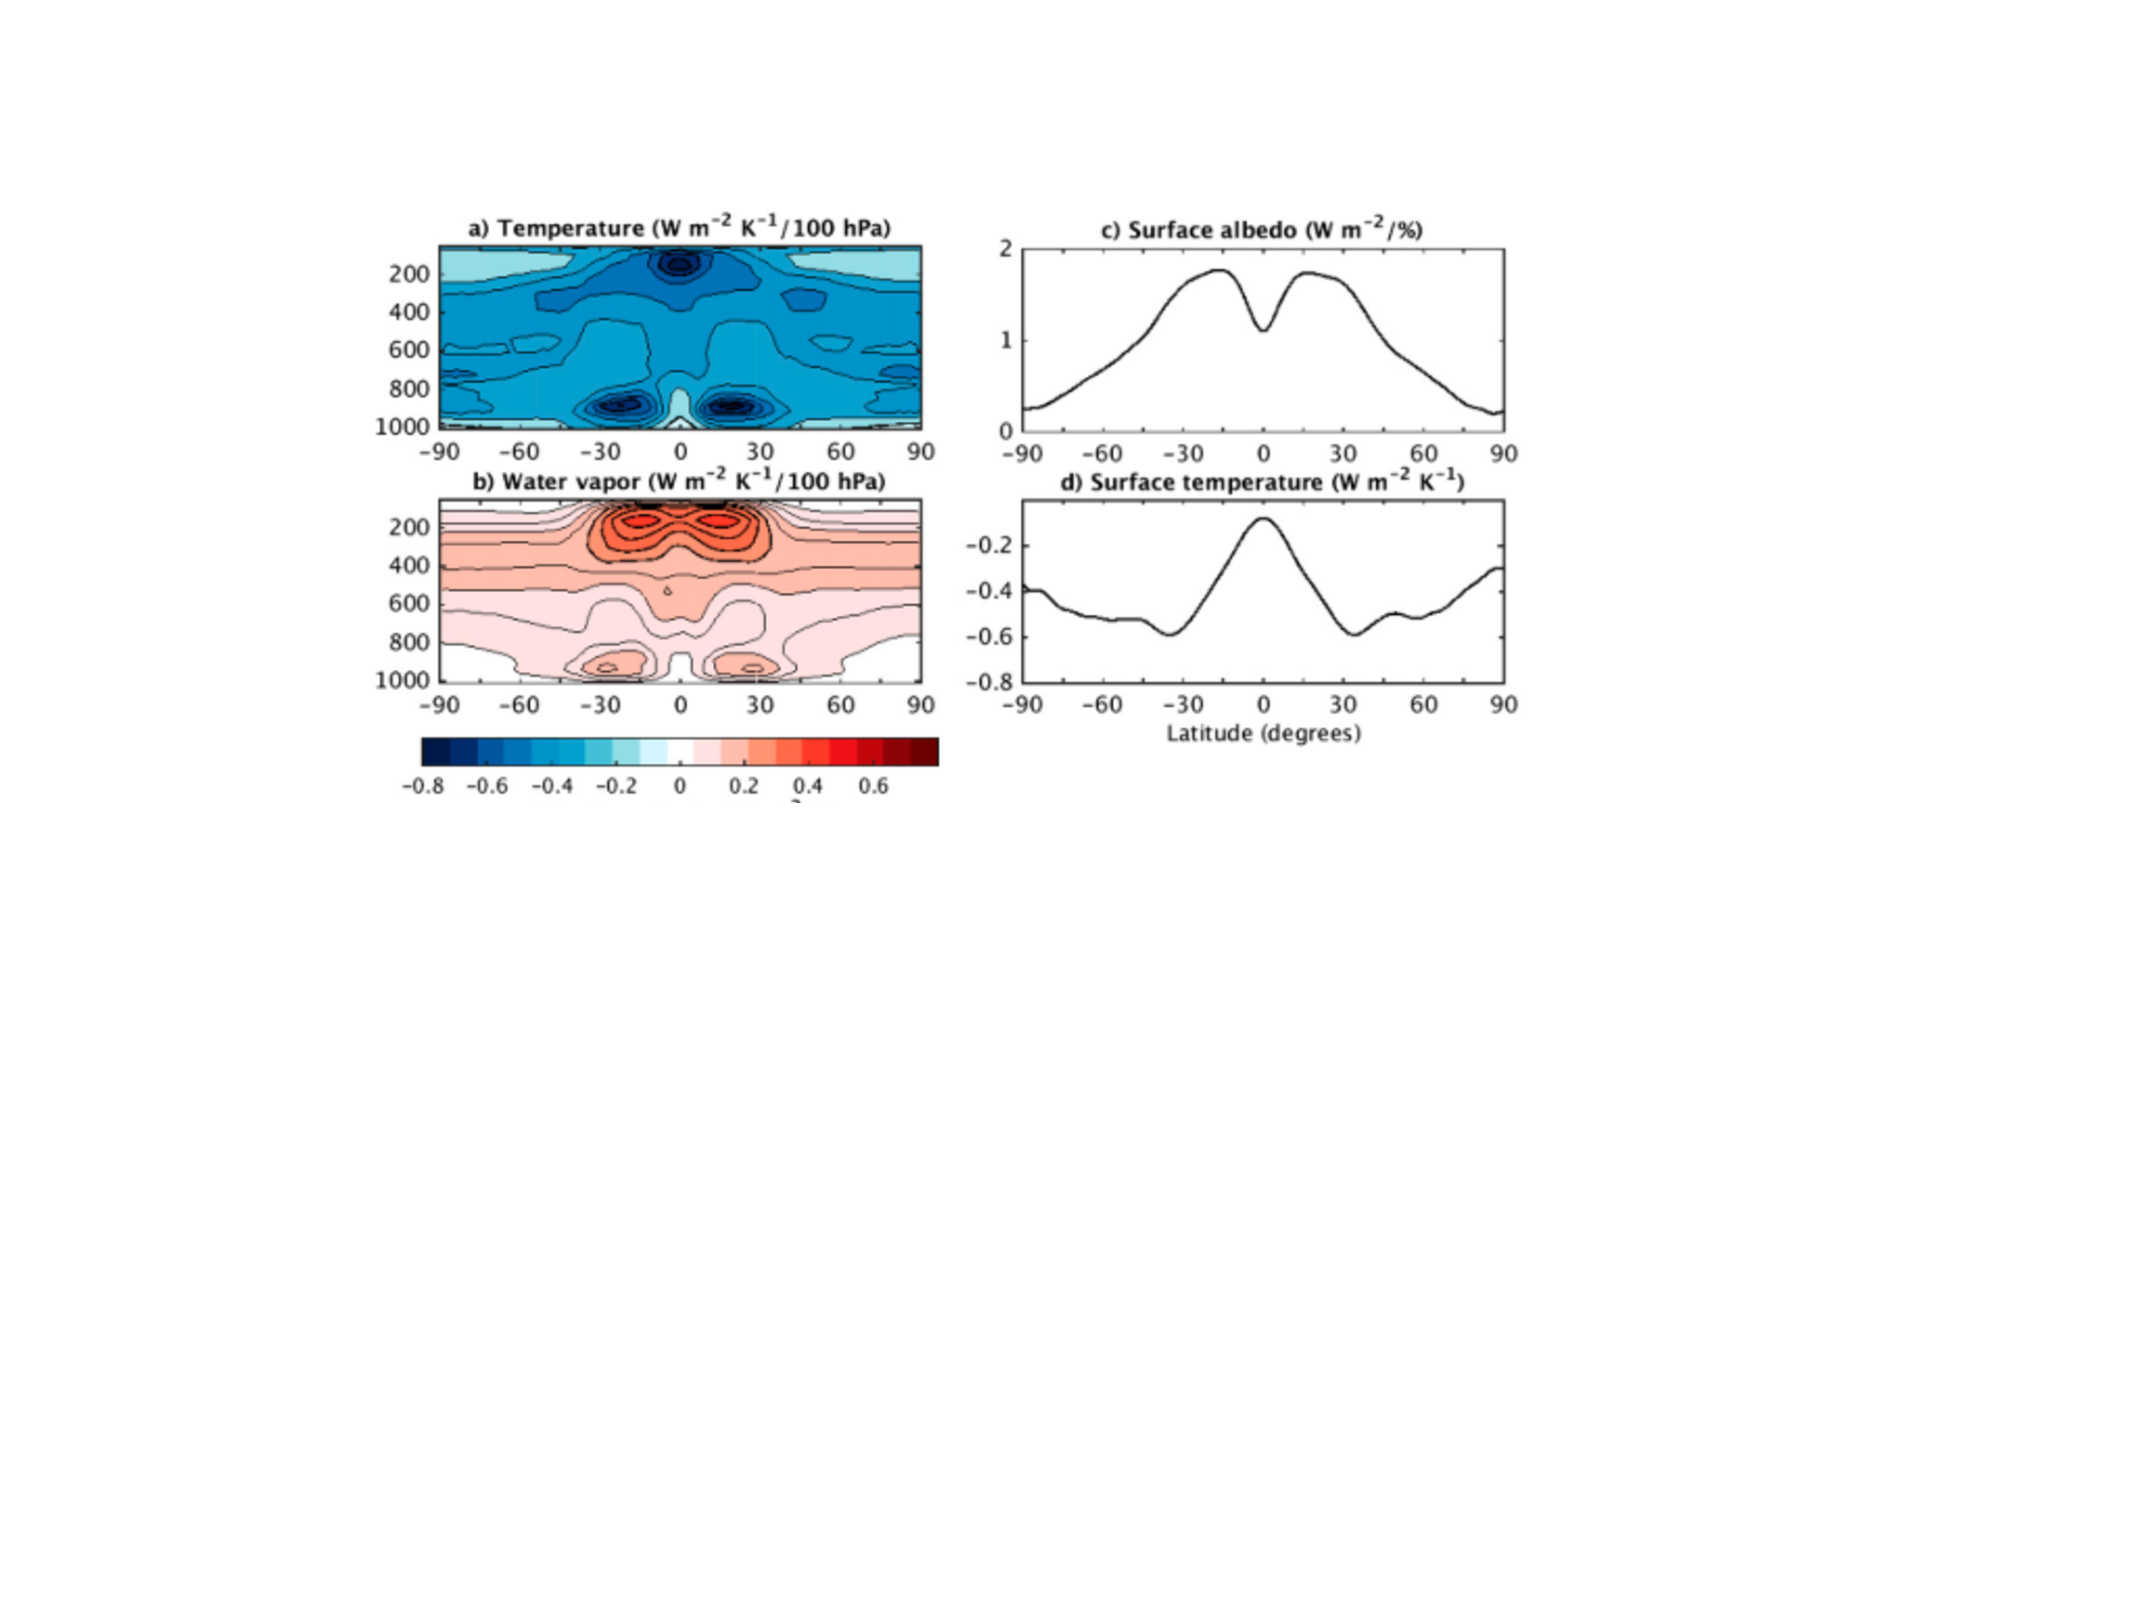
\includegraphics[width=.8\linewidth]{figs/polar_amp/Feldl2017}
% 	\caption[Annual-mean, zonal-mean radiative kernels for the GFDL AM2.1]{Annual-mean, zonal-mean radiative kernels for the GFDL AM2.1 aquaplanet based on a $4\times$ CO$_2$ simulation with daily mean solar zenith angle: (a) temperature kernel [W m$^{-2}$ K$^{-1}$ / 100 hPa], (b) water vapor kernel for a specific humidity perturbation corresponding to a 1-K temperature increase and fixed relative humidity, (c) surface albedo kernel, and (d) surface component of the temperature kernel. Adapted from Figure A1 of \cite{Feldl2017coupled}.}
% 	\label{fig:feldl_gfdl_am2.1_kernel}
% \end{figure}

\begin{figure}[ht]
	\centering
	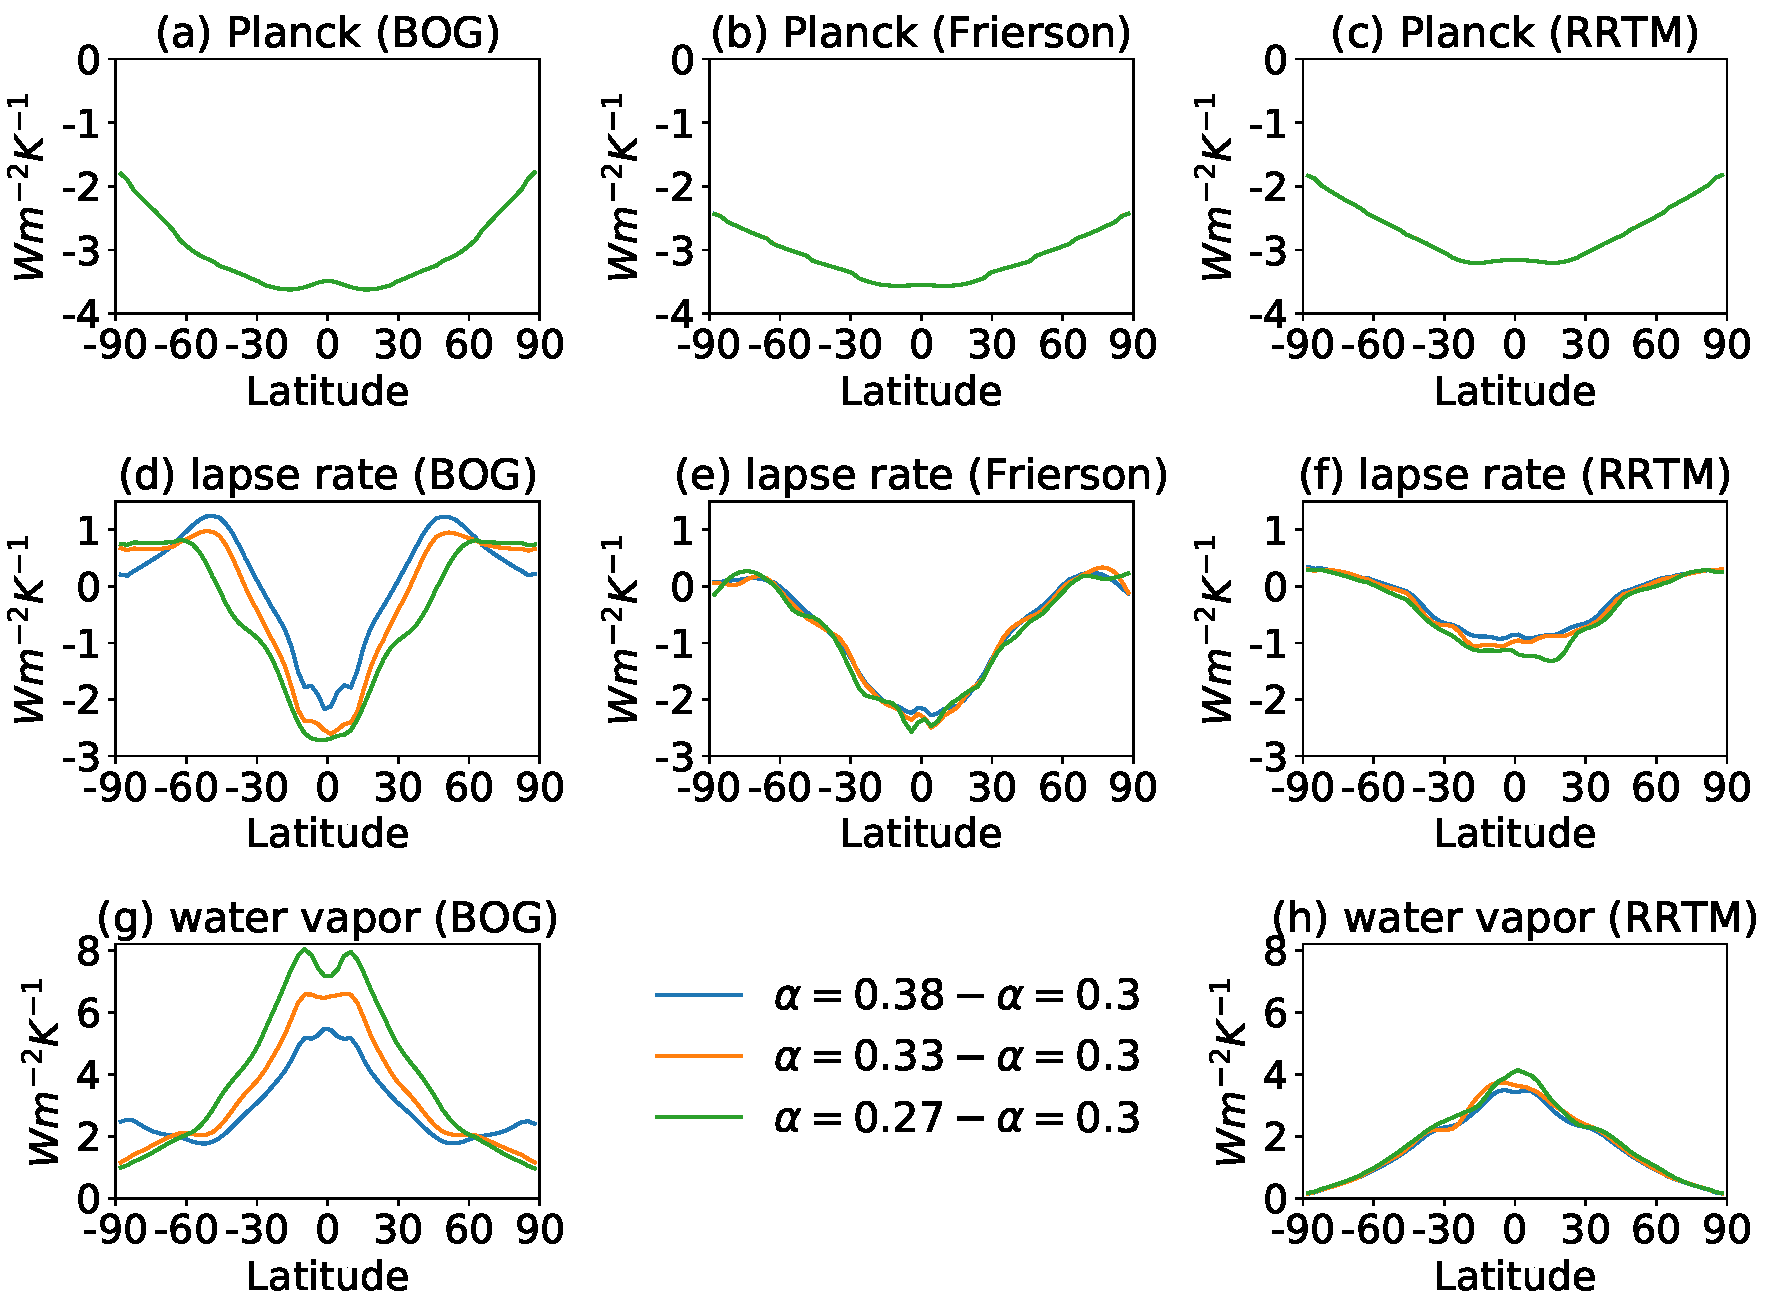
\includegraphics[width=0.8\textwidth]{figs/polar_amp/all_zonalmean_feedbacks}
	\caption[The zonal and annual mean climate feedback parameters for all the experiments in BOG, Frierson and RRTM radiation schemes]{The zonal and annual mean climate feedback parameters for all the experiments in BOG, Frierson and RRTM radiation schemes, where (a)-(c) are for the Planck feedbacks, (d)-(f) for the lapse rate feedbacks and (g)-(h) for the water vapor feedbacks. Blue, orange and green lines represent the experiments when albedo ($\alpha$) is changed from 0.3 to 0.38, 0.33 and 0.27 respectively.}
	\label{fig:all_feedbacks}
\end{figure}

\subsection{Climate feedbacks in Isca}
For each radiation scheme, the albedo parameter is changed from 0.3 to 0.27, 0.33 and 0.38 to provide an external forcing to the simulation respectively, leading to different degree of climate responses in experiments. Thus in this section, we will use the radiative kernel technique to analyze the feedbacks for these experiment when changing albedos and the resulting Planck feedback, lapse rate feedback and water vapor feedback for each experiments are displayed in \figref{fig:all_feedbacks}.

% \begin{table}[ht]
% 	\centering
% 	\small
% 	\caption{Global mean lapse rate feedback parameters (Units: W m$^{-2}$ K$^{-1}$).}
% 	\vspace{0.5em}
% 	\label{tab:lapserate_fb}
% 	\begin{tabular}{cccc}
% 		\toprule
% 		Experiment & BOG & Frierson & RRTM \\
% 		\midrule
% 		$\alpha=$0.38 $-$ $\alpha=$0.3 & -0.33 & -1.23 & -0.51 \\
% 		$\alpha=$0.33 $-$ $\alpha=$0.3 & -0.84 & -1.28 & -0.61 \\
% 		$\alpha=$0.27 $-$ $\alpha=$0.3 & -1.15 & -1.32 & -0.72\\
% 		\bottomrule
% 	\end{tabular}
% \end{table}

% \begin{table}[ht]
% 	\centering
% 	\small
% 	\caption{Global mean water vapor feedback parameters (Units: W m$^{-2}$ K$^{-1}$).}
% 	\vspace{0.5em}
% 	\label{tab:wv_fb}
% 	\begin{tabular}{ccc}
% 		\toprule
% 		Experiment & BOG & RRTM \\
% 		\midrule
% 		$\alpha=$0.38 $-$ $\alpha=$0.3 & 3.38 & 2.14\\
% 		$\alpha=$0.33 $-$ $\alpha=$0.3 & 4.21 & 2.23 \\
% 		$\alpha=$0.27 $-$ $\alpha=$0.3 & 5.03 & 2.41\\
% 		\bottomrule
% 	\end{tabular}
% \end{table}

\begin{table}[ht]
	\centering
	\small
	\caption{Global mean lapse rate and water vapor feedback parameters (Units: W m$^{-2}$ K$^{-1}$).}
	\vspace{0.5em}
	\label{tab:lapserate_and_wv_fb}
	\begin{tabular}{cccccc}
		\toprule
		\multirow{2}{*}{Experiment} & \multicolumn{3}{c}{Lapse rate} & \multicolumn{2}{c}{Water vapor} \\\cline{2-4}\cline{5-6}
		{} & BOG & Frierson & RRTM & BOG & RRTM\\
		\midrule
		$\alpha=$0.38 $-$ $\alpha=$0.3 & -0.33 & -1.23 & -0.51 & 3.38 & 2.14 \\
		$\alpha=$0.33 $-$ $\alpha=$0.3 & -0.84 & -1.28 & -0.61 & 4.21 & 2.23 \\
		$\alpha=$0.27 $-$ $\alpha=$0.3 & -1.15 & -1.32 & -0.72 & 5.03 & 2.41 \\
		\bottomrule
	\end{tabular}
\end{table}

The Planck feedback \index{Feedback!Planck} is negative in all latitudes (\figsref{fig:all_feedbacks}a-c), meaning that an increase in temperature can increase the outgoing longwave radiation. In addition, the strength of Planck feedback in polar region is weaker than the tropical region due to smaller blackbody emissions per unit warming at lower temperatures according to Stefan-Boltzmann law \citep{Goosse2018}. The global mean Planck feedback parameters are -3.82, -3.79 and -3.41 W m$^{-2}$ K$^{-1}$ for BOG, Frierson and RRTM radiation schemes respectively, showing that the differences of Planck feedbacks in different radiation schemes are small. Regarding the lapse rate feedbacks, they are negative in low latitudes but positive in high latitudes, which is due to the different vertical distribution of temperature change in polar region compared to the tropics, as the temperature change is bottom heavy in polar regions \citep{Pithan2014}. The global mean lapse rate feedback parameters for all experiments and all radiation schemes are listed in \tabref{tab:lapserate_and_wv_fb}. It is clear that the difference of global mean lapse rate feedbacks among different radiation schemes is large, but is small within the experiments with same radiation schemes, except the one where albedo is 0.38 in BOG radiation scheme. As for water vapor feedback, it is positive in all experiments, implying that the net incoming longwave radiation increase in response to temperature warming. However, the spatial distribution of water vapor feedback is nonuniform, with high feedback in tropics and small values in polar regions (\figsref{fig:all_feedbacks}g and \ref{fig:all_feedbacks}h). This is because of the nonlinear effect of water vapor in response to warming. In addition, the global mean water vapor feedback parameters are displayed in \tabref{tab:lapserate_and_wv_fb}, where the water vapor feedback in BOG schemes is almost twice of feedbacks in RRTM scheme and the later is close to the water vapor feedback (2.01 W m$^{-2}$ K$^{-1}$) estimated by \cite{Soden2008} in GFDL AM2p12b, indicating that the water vapor feedback is much stronger in BOG radiation scheme.

%%%%%%%%%%%%%%%%%%%%%% New section %%%%%%%%%%%%%%%%%%%%%%

\section{Results}
\label{sec:polar_amiplification_results}

%\subsection{Climate response}
\subsection{Surface temperature response}
\begin{figure}[ht]
	\centering
	%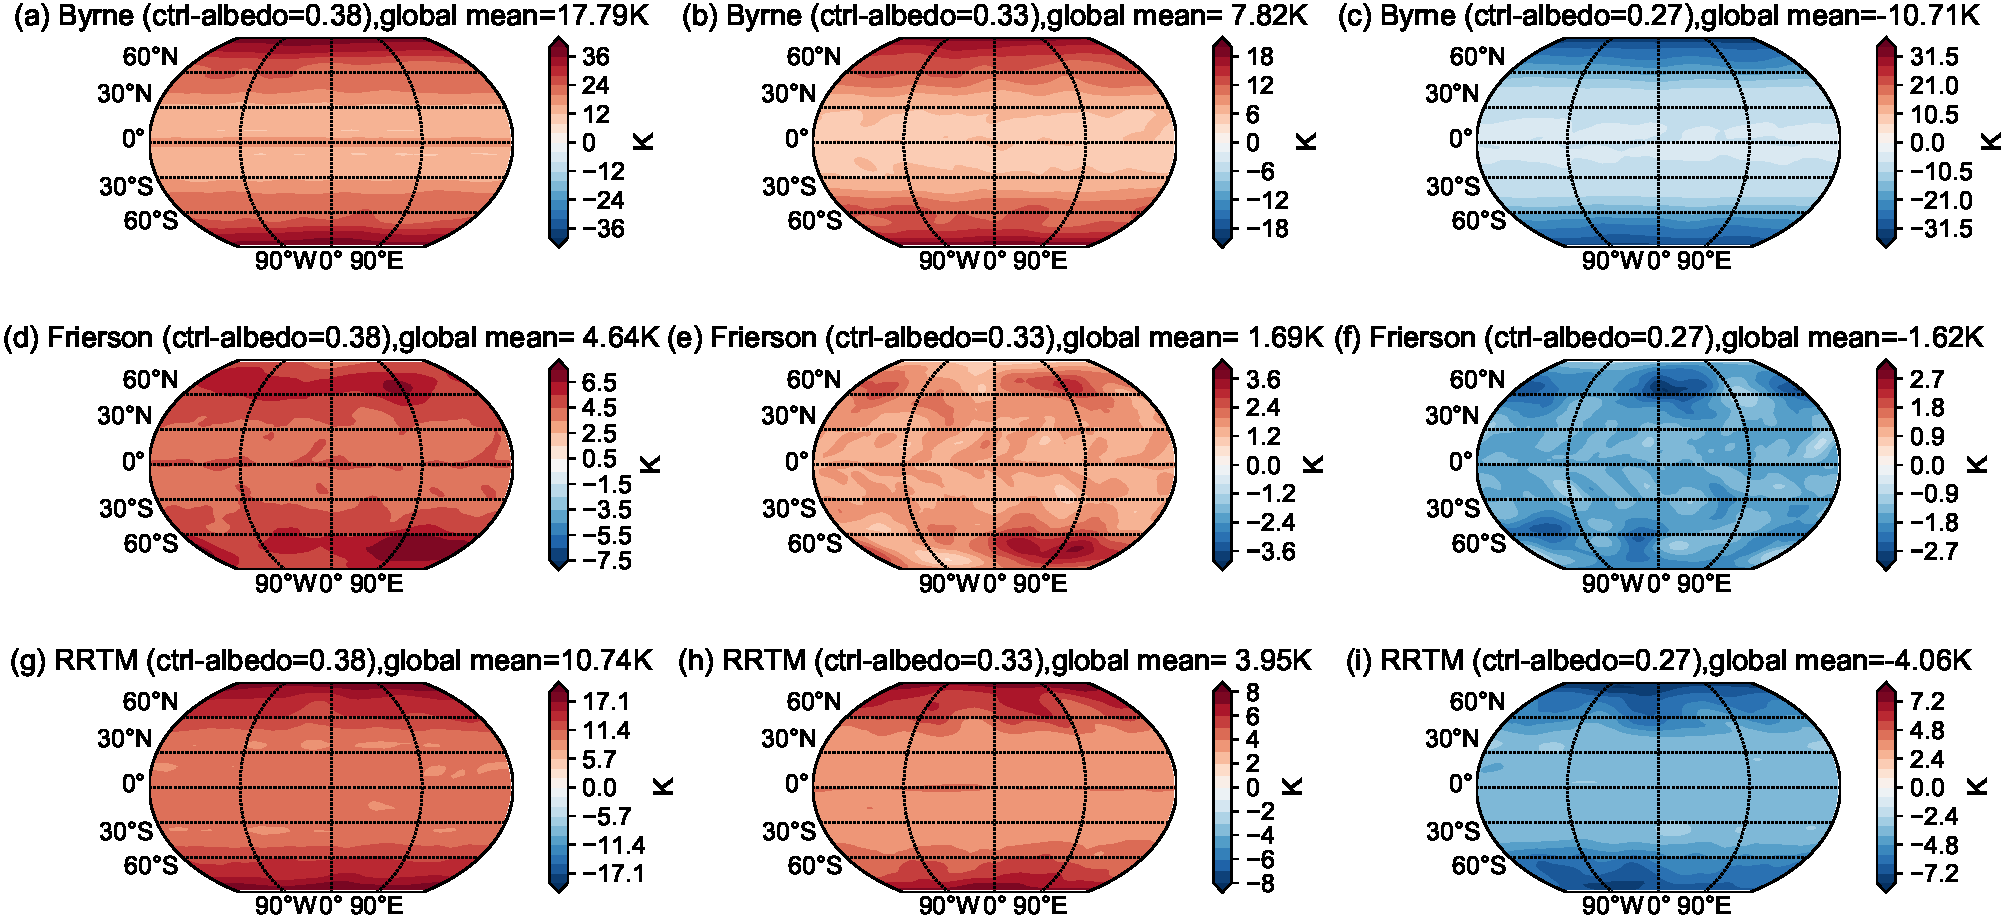
\includegraphics[width=1.0\linewidth]{{figs/polar_amp/tsurf_diff_ctrl_m_others_RdBu_kav7}.pdf}
	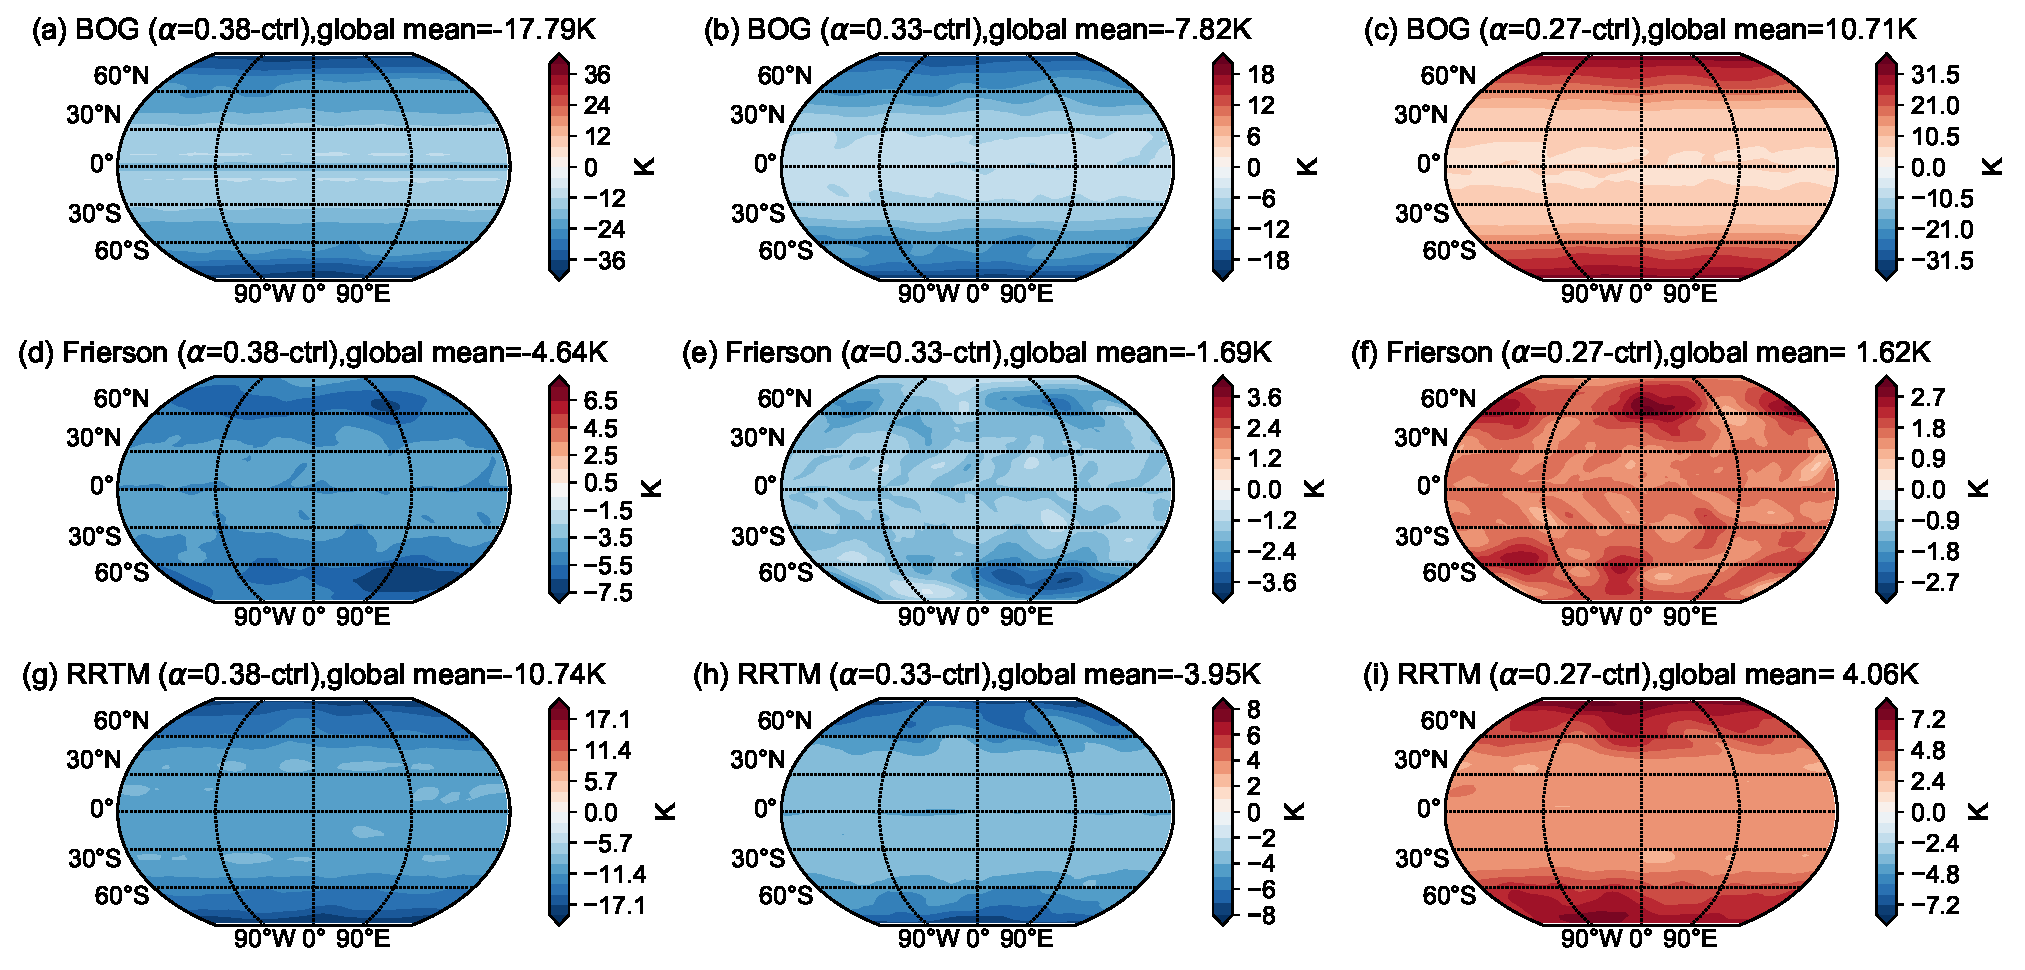
\includegraphics[width=1.0\linewidth]{{figs/polar_amp/tsurf_diff_others_m_ctrl_RdBu_kav7_2}.pdf}
	\caption[The spatial patterns of annual-mean surface temperature changes]{The global patterns of annual-mean surface temperature differences between the runs after changing albedos and the control run (i.e. $\alpha=0.3$) for (a-c) BOG, (d-f) Frierson and (g-i) RRTM radiation schemes respectively, where the (a, d, g) left, (b, e, h) middle and (c, f, i) right panels represent the runs in which albedos are changed from 0.3 to 0.38, 0.33 and 0.27 respectively.}
	\label{fig:tsurf_diff}
\end{figure}

The global patterns of annual mean surface temperature differences after changing albedos for the BOG, Frierson and RRTM radiation schemes are displayed in \figref{fig:tsurf_diff}. The BOG scheme produces the largest surface temperate changes compared to the other two radiation schemes and Frierson scheme produces the weakest responses. For example, the annual and global mean surface temperature difference is 10.71K in experiment where the albedo decreased 10\% from control run (i.e. from 0.3 to 0.27) for BOG scheme. Global mean values are only 4.06K and 1.62K for RRTM and Frierson schemes. Despite the responses are in a relative wide ranges, all simulation results from the three radiation schemes show polar amplified patterns either in cooling or warming situations, which are clearly shown in the  annual and zonal mean patterns (\figsref{fig:delta_ts}a-c). The striking feature is that the strongest polar amplification pattern appears in the BOG scheme. However, the zonal mean surface temperature change in Frierson scheme is almost flat with slight amplified cooling or warming at high latitudes but not exactly at the poles. Like the global mean surface temperature changes, the zonal mean patterns and the polar amplification are also moderate in RRTM scheme among the three schemes.

To make the feature more evident, the zonal mean surface temperature responses are also normalized by the change in global mean surface temperature (\figsref{fig:delta_ts}d-f), showing that results from Frierson scheme also have a slight polar amplification. Generally, the Arctic warming is almost twice as large as the global average in recent decades \citep{Serreze2006}. For example, the Arctic has a warming 1.9 times that of the globe on average in twelve IPCC AR4 models in CO$_2$ doubling experiments \citep{Winton2006surface}. As for the observed Arctic warming in the last half century, the zonal-mean Arctic warming is roughly 3 times compared to tropical warming \citep{Merlis2018}. All results suggest that the ratios between polar and global temperature response seem a little surprising due to the lack of some feedback mechanisms such as surface albedo feedback in our experiments.

%% This weired behavior is due to the Q-flux, ocean heat transport...
% One strange thing in BOG scheme is that annual and zonal mean surface temperature change in equator exhibits larger cooling relative to elsewhere in tropics, for which the reasons will be investigated later. 
% 
%  and strongest polar amplification  showing various amplitudes in the surface temperature change

% Although the forcing changes by altering albedo differ from the way to double CO$_2$, the experiments illustrate that polar amplification can exist even in aquaplanet models.
% The zonal-mean and annual-mean surface temperature changes for each radiation scheme and albedo are presented in the,
%These results can also be quantified by the ratio between the surface temperature change in Arctic region and the globe or tropical region. 

%\begin{figure}[ht] %[ht]
%	\centering
%	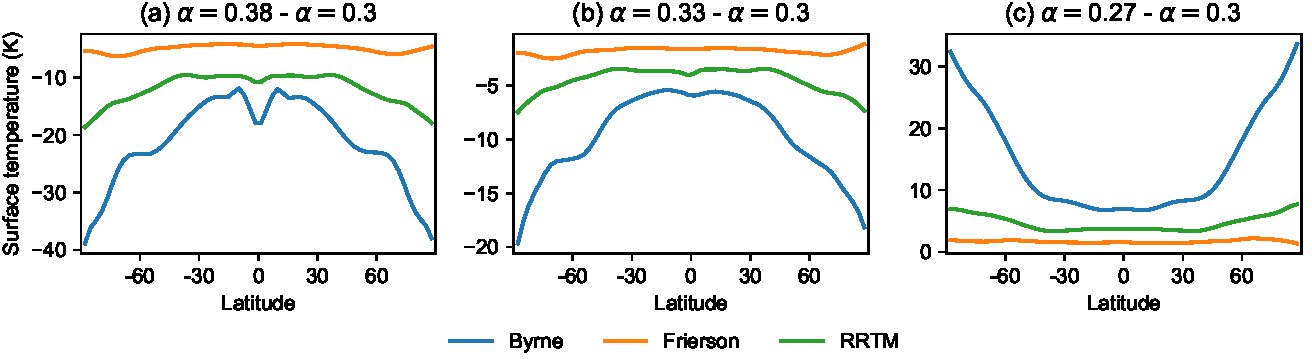
\includegraphics[width=1.0\linewidth]{{figs/polar_amp/tsurf_diff_zonal_mean_others_m_ctrl}.pdf}
%	\captionof{figure}{Temperatue difference when changing the global mean albedos (Annual and Zonal mean).}
%	\label{fig:tsuf_diff_zonal}
%\end{figure}

\begin{figure}[ht] % [ht]
	\centering
	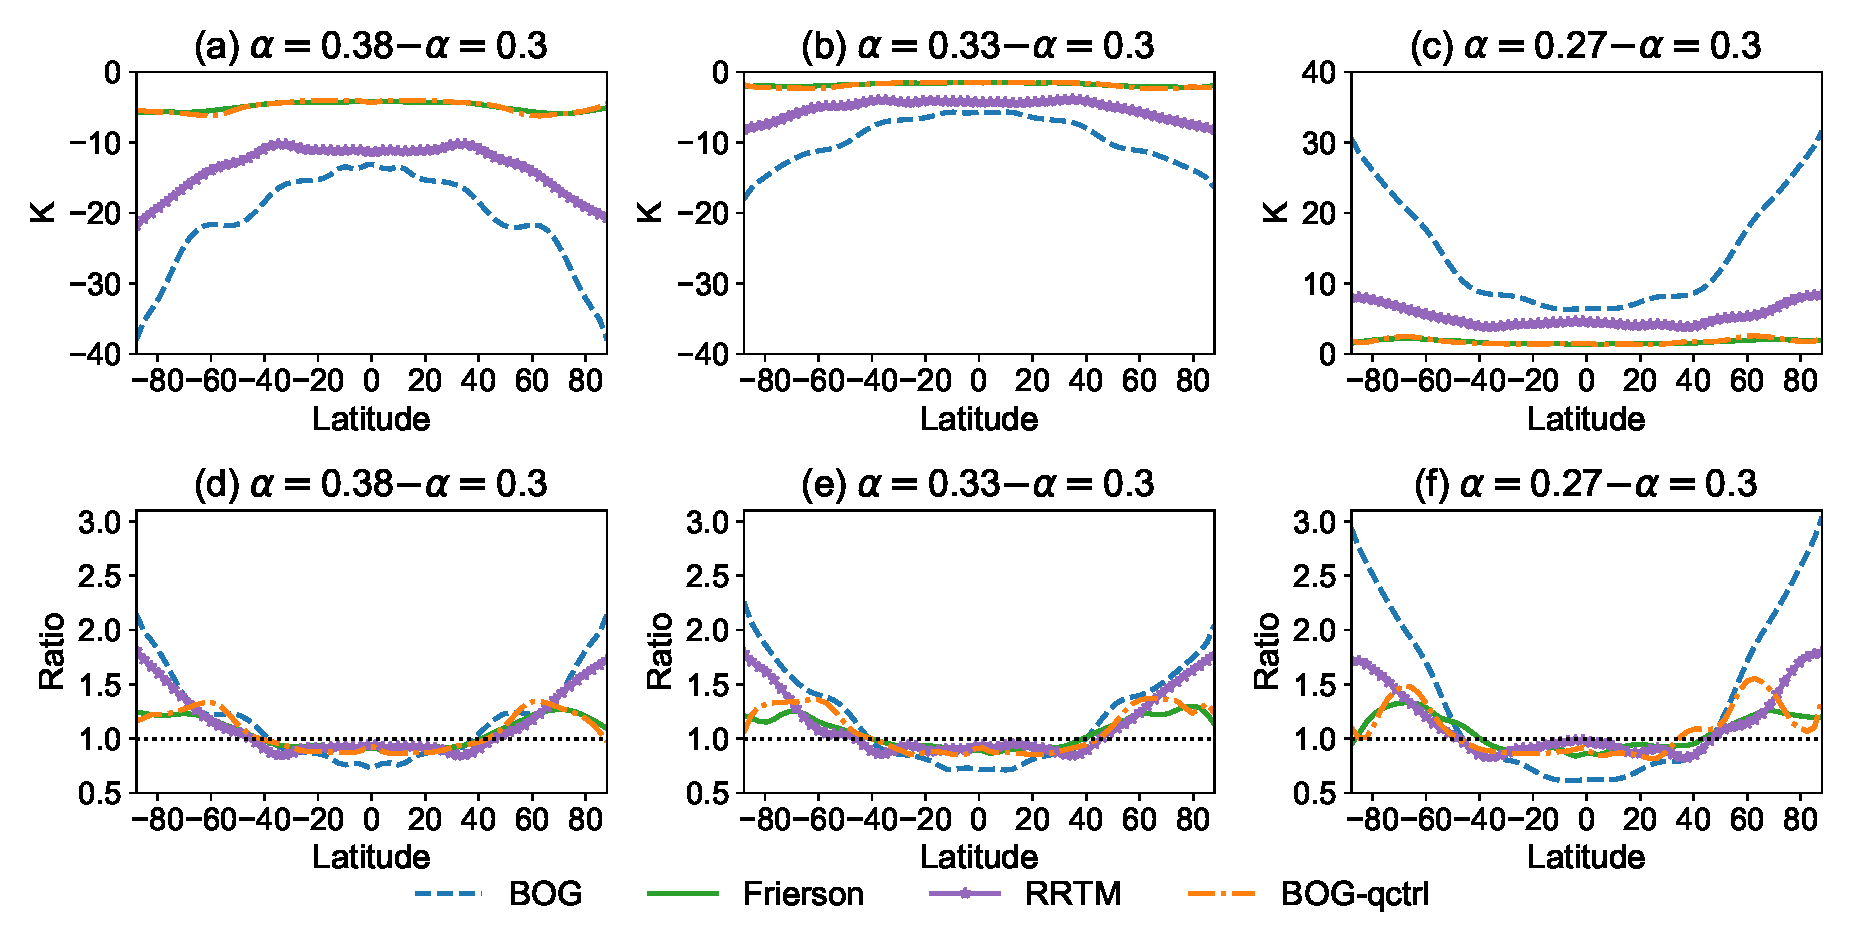
\includegraphics[width=1.0\linewidth]{figs/polar_amp/ts_diff.pdf}
	\caption[The zonal and annual mean surface temperature changes (top) and the change ratios with respect to global mean surface temperature change (bottom)]{The zonal mean and annual mean surface temperature changes for experiments where albedo is changed from 0.3 to (a) 0.38, (b) 0.33 and (c) 0.3 respectively. Correspondingly, (d)-(f) show the ratios of surface temperature change at each latitude to the global mean surface temperature change for different simulations. Each experiment has been run in the BOG (blue dashed line), Frierson (green solid line) and RRTM (purple solid-starred line) radiation schemes respectively. The orange dash-dotted lines denote the experiments in BOG scheme without moisture feedback.}
	\label{fig:delta_ts}
\end{figure}

\begin{figure}[ht] 
	\centering
	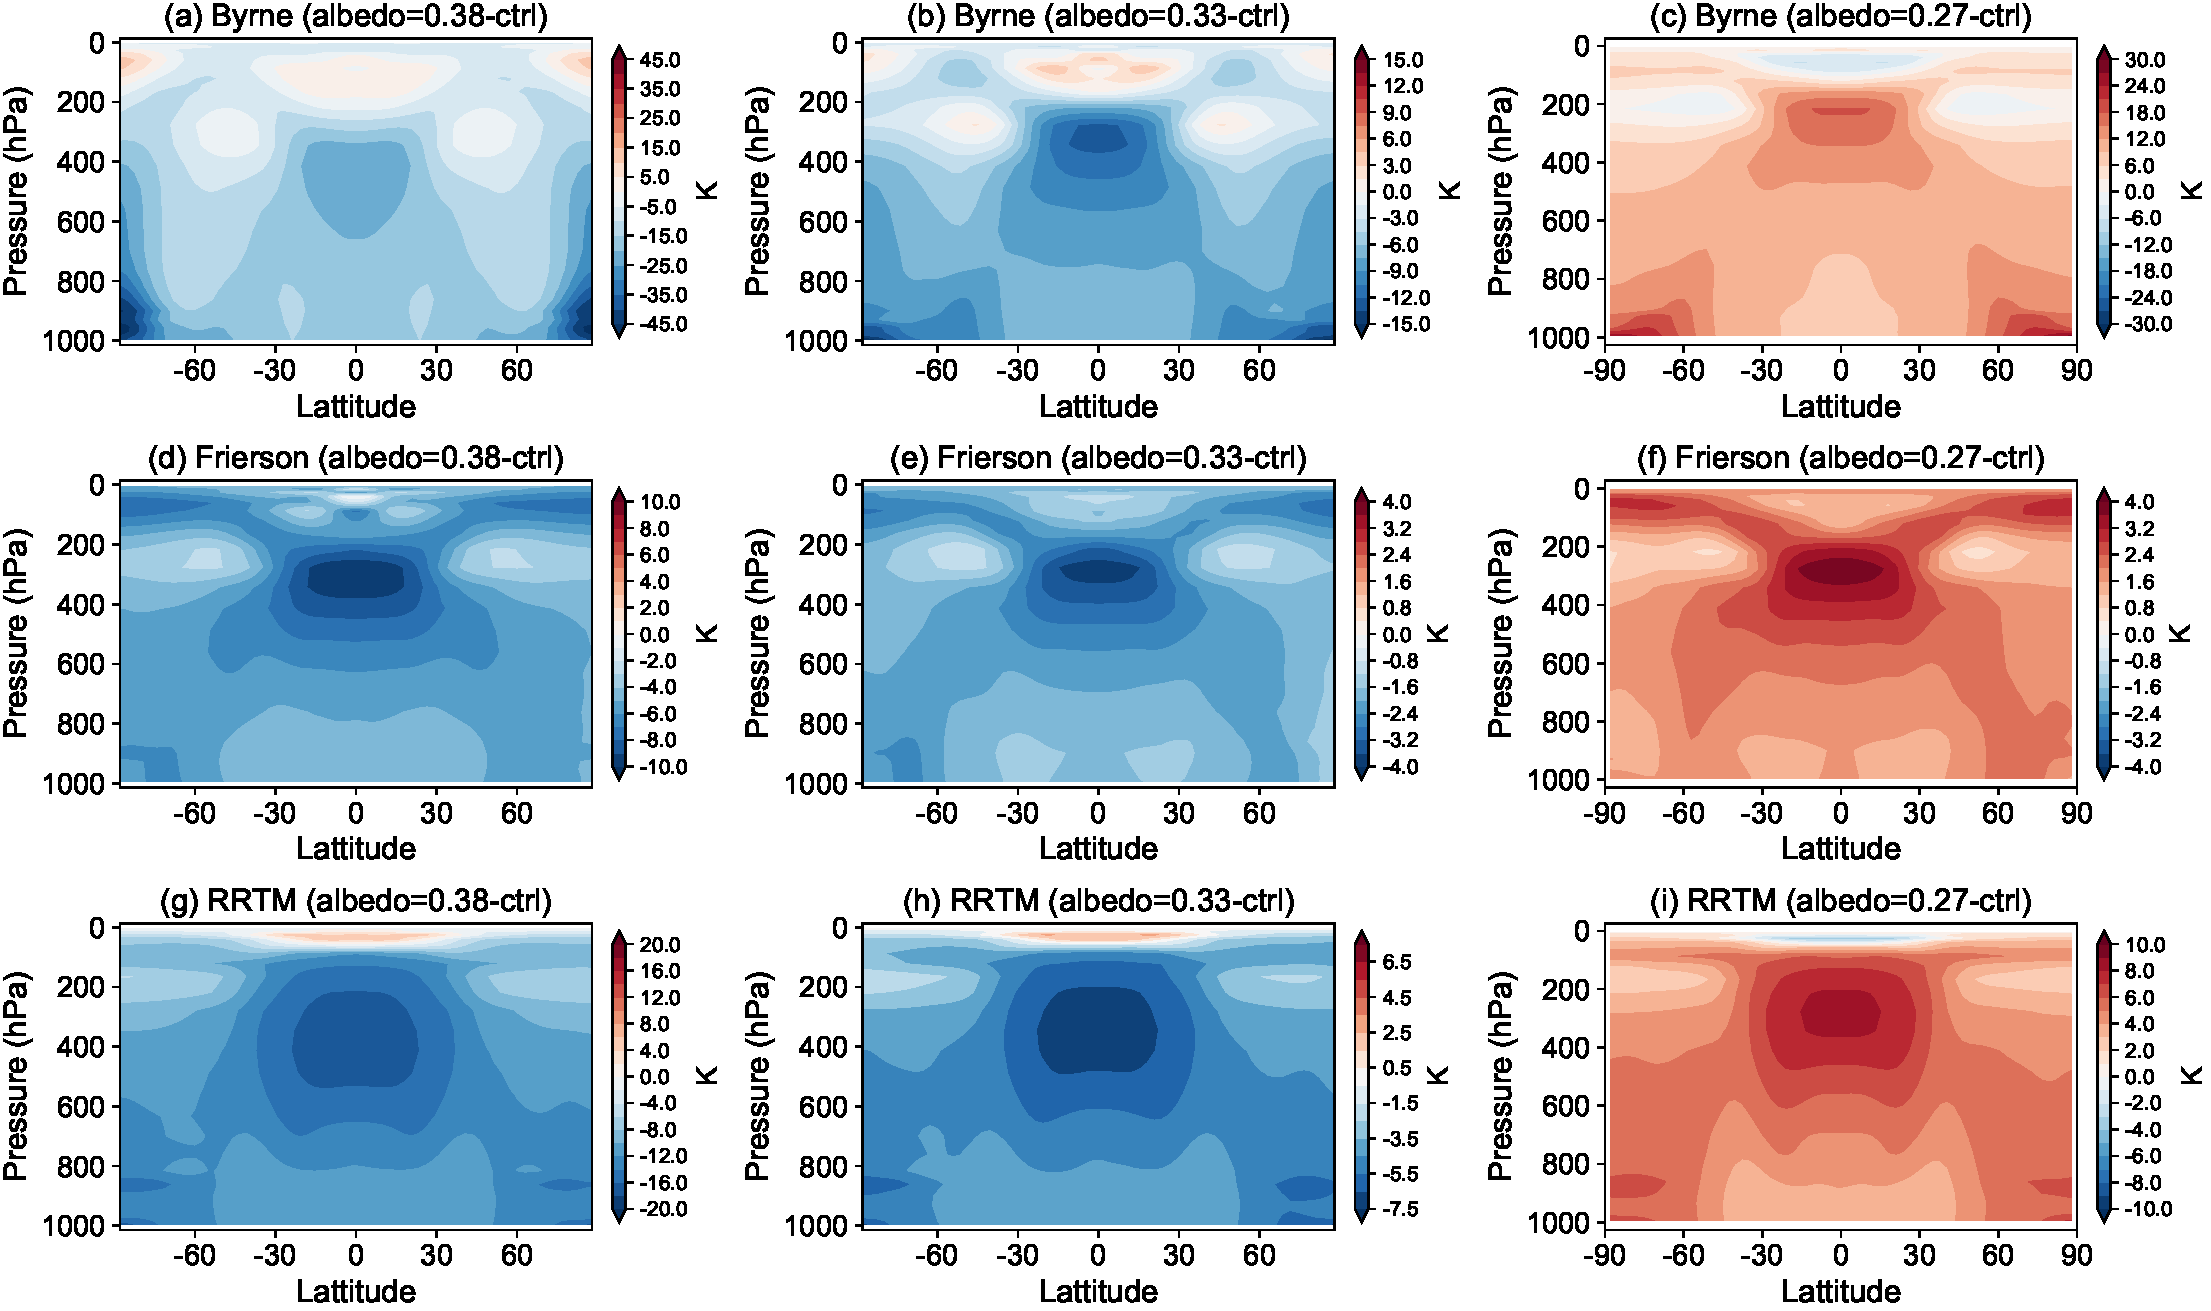
\includegraphics[width=1.0\linewidth]{{figs/polar_amp/temp_vert_profile_diff_others_m_ctrl_RdBu_symmetric}.pdf}
	\caption[The annual and zonal mean profiles of atmospheric temperature change]{The annual mean atmospheric temperature change profiles for experiments in (a)-(c) BOG, (d)-(f) Frierson and (g)-(i) RRTM radiation schemes. The (a, d, g) left, (b, e, h) middle and (c, f, i) right panels are for the experiments where albedos are altered from	 0.3 (control run) to 0.38, 0.33 and 0.27 respectively.}
	\label{fig:vert_temp_diff}
\end{figure}

%\caption{The annual and regional mean temperature differences in Arcitc and tropical regions and their warming (or cooling) ratio when changing the global mean albedos.}
% \begin{table}[ht]
	% \centering
	% \caption{The annual and regional mean temperature differences in  Arcitc and tropical regions and their warming (or cooling) ratio when changing the global mean % albedos.}
	% \begin{adjustbox}{width=1.0\textwidth,center=\textwidth}
	% \begin{tabular}{l c c c c c c c c c}
		% \toprule
		% \multirow{2}{*}{Region} & \multicolumn{3}{c}{Byrne(albedo=$x$-ctrl)} & \multicolumn{3}{c}{Frierson(albedo=$x$-ctrl)} & \multicolumn{3}{c}{RRTM(albedo=$x$-ctrl)}%  \\
		% \cline{2-4}  \cline{5-7} \cline{8-10}
		% & $x$=0.38 & $x$=0.33 & $x$=0.27 & $x$=0.38 & $x$=0.33 & $x$=0.27 & $x$=0.38 & $x$=0.33 & $x$=0.27\\
		% \midrule
		% Arctic & -30.53 & -14.47 & 26.70 & -5.52 & -1.87 & 1.94 & -15.13 & -5.99 & 6.36\\
		% Tropics & -14.64 & -5.69 & 6.86 & -4.35 & -1.58 & 1.52 & -10.12 & -3.72 & 3.71\\
		% Ratio & 2.09 & 2.54 & 3.89 & 1.27 & 1.19 & 1.27 & 1.50 & 1.61 & 1.72\\
		% \bottomrule
	% \end{tabular}
	% \end{adjustbox}
% \end{table}

To better understand the surface temperature responses, the structures of vertical atmospheric temperature changes are also investigated. As shown in \figref{fig:vert_temp_diff}, it is obvious that bottom-heavy cooling or warming profiles appear in polar regions (\figsref{fig:delta_t_profile}a-c) in all the experiments, but top-heavy cooling or warming profiles appear in tropical upper troposphere (\figsref{fig:delta_t_profile}d-f). Many studies have found that these bottom-heavy structure is associated with polar amplification \citep{Screen2012, Pithan2014, Kim2018, Park2018}, as the stability in polar region can trap more heat at the surface in warming case, which hence leads to the positive lapse rate feedback in polar region (\figsref{fig:all_feedbacks}d-f). In contrast, the lapse rate feedback is negative in tropics, which means that in a warming climate, more latent heat will be released in upper troposphere and thus cause greater warming in the upper troposphere than at the surface \citep{Pithan2014}.

It is worth noting that the sea ice is responsible for the stable atmospheric structure in polar region in the real world, but the stability of polar region in our study is due to the equinox solar radiation. \cite{Kim2018} studied the sensitivity of polar amplification to insolation conditions and found that the equinox insolation brings the largest static stability than seasonal or annual mean conditions due to the year-round near zero solar radiation reaching the polar region. Taking the warming case as an example, the active convection in the tropics induces a tight coupling between surface and upper troposphere, and the rising air parcel in warming climate will release more latent heat in upper troposphere, decreasing the moist lapse rate \citep{Graversen2014}. Instead, the polar region is more stable and mixing with air aloft is harder than in tropics, so that more heat is trapped near surface, leaving a bottom heavy temperature structure and positive lapse rate feedback \citep{Pithan2014}. What is more, if we check closely the bottom heavy profile in Frierson scheme, the largest warming or cooling near surface occurs at about 70 degree not the poles (\figsref{fig:vert_temp_diff}d-f), which explains largest value of the zonal mean surface temperature change in Frierson scheme in \figref{fig:delta_ts}.


In summary, polar amplification can exist in the aquaplanet model even without the sea ice and surface albedo feedback. Regarding the three radiation schemes we used in this study, the polar amplification of surface temperature is strongest in BOG scheme, moderate in RRTM and weakest in Frierson scheme. As mentioned in \secref{sec:wv_fb_setup}, the crucial distinction between BOG and Frierson is whether there is moisture feedback in their longwave radiation schemes, which will be discussed in further in \secref{sec:wv_feedback}. On the mechanisms about polar amplification, the bottom heavy structure of temperature difference provides some reasonable explanations for the polar amplification via lapse rate feedback, which will be investigated further in \secref{sec:climate_feedbacks_temp_decomp}.

\begin{figure}[ht]
	\centering
	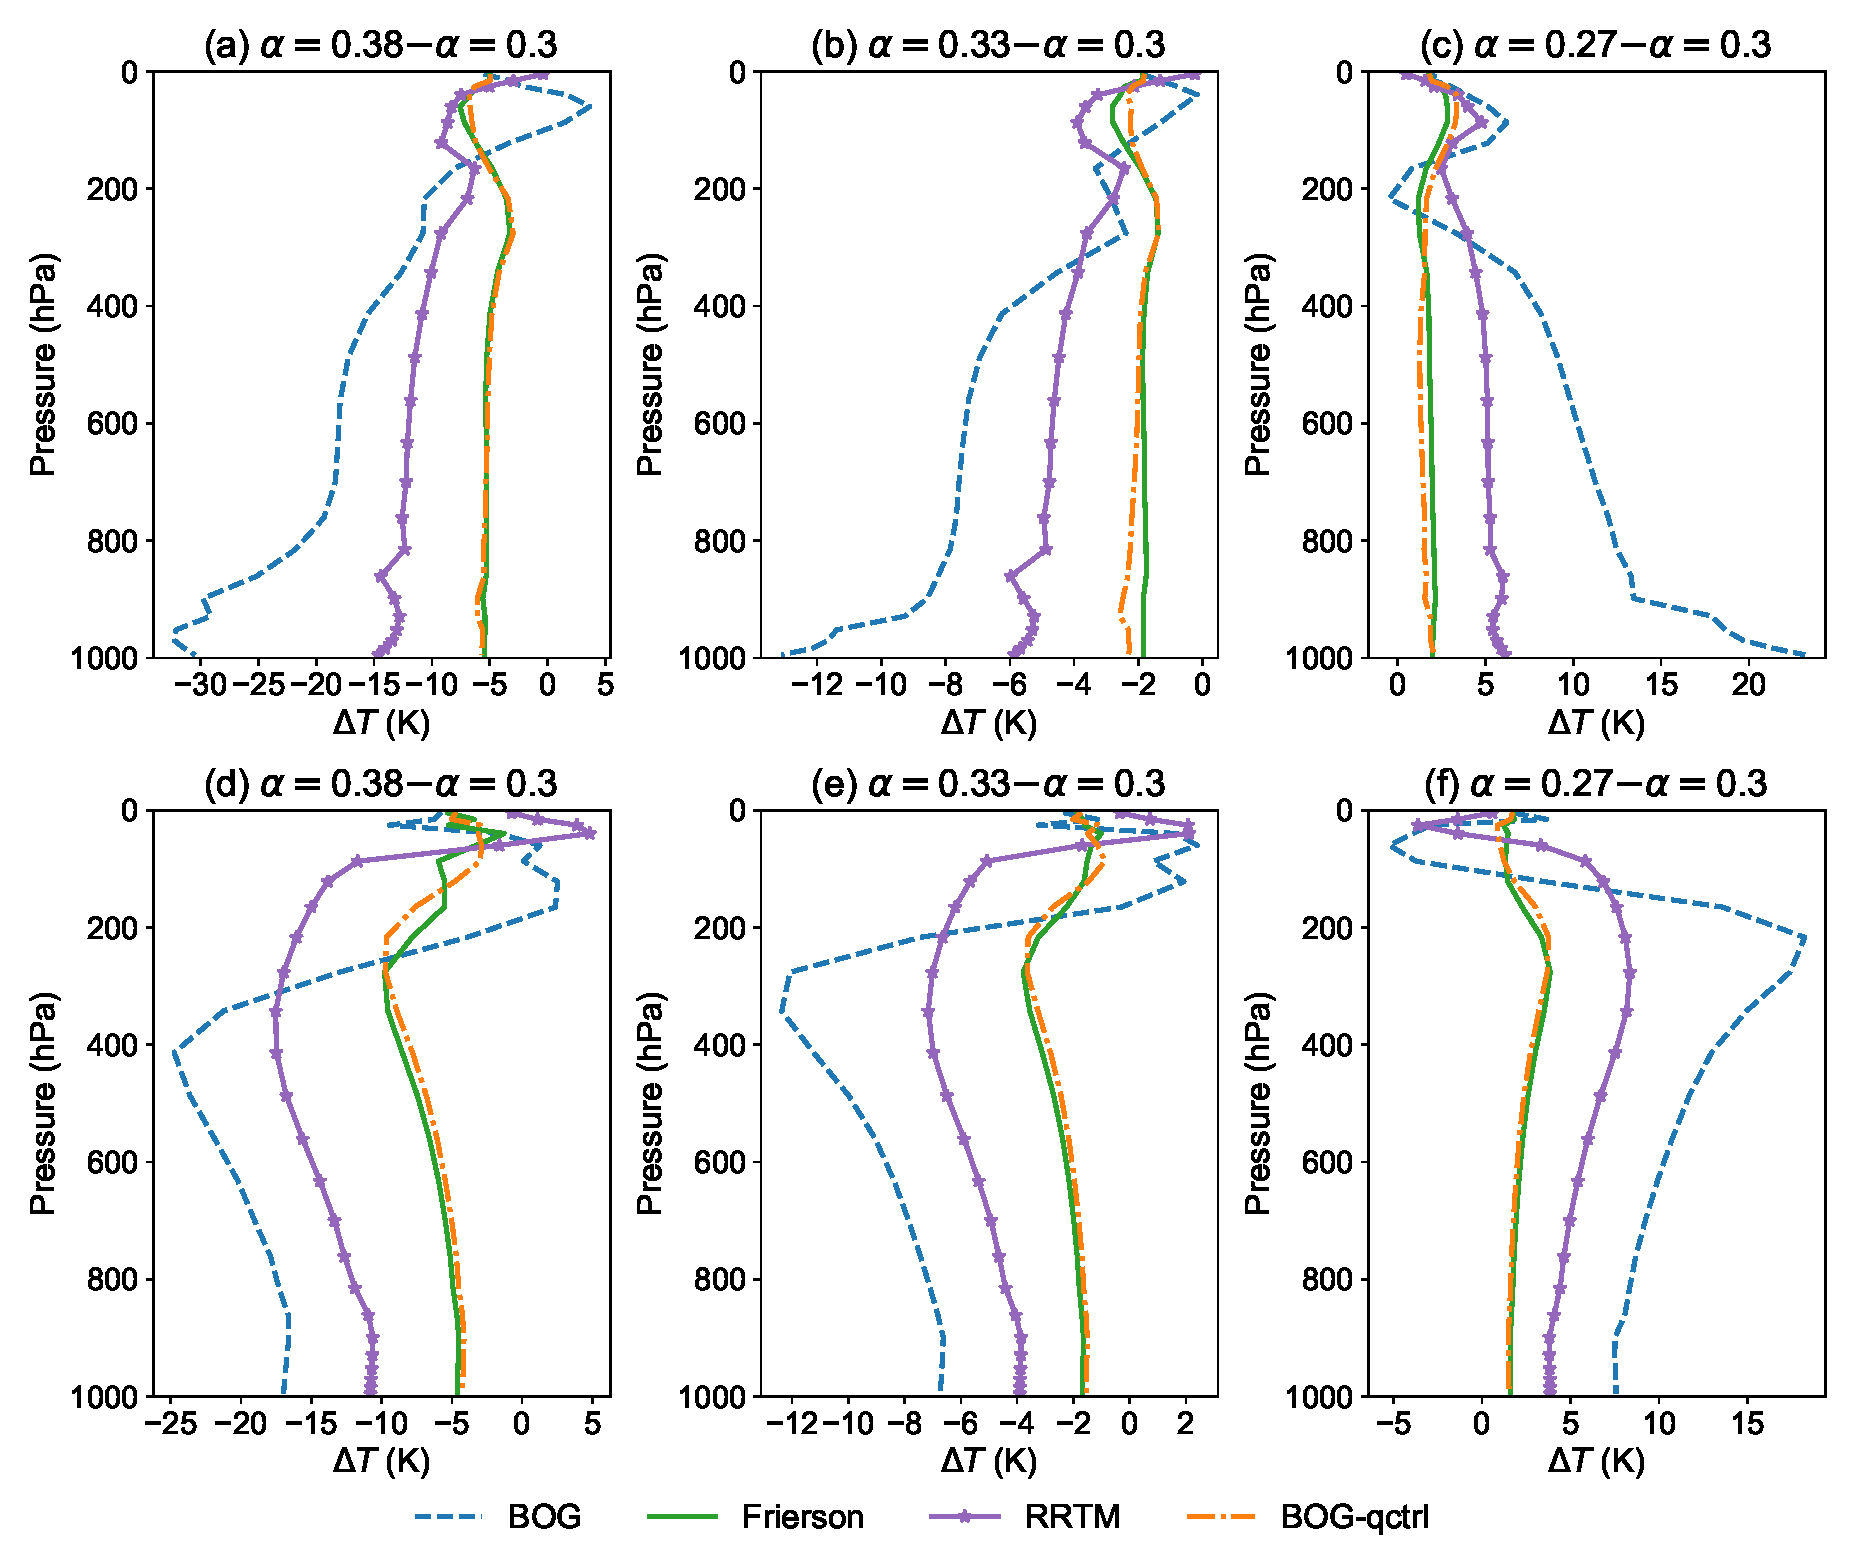
\includegraphics[width=0.8\linewidth]{figs/polar_amp/temp_profile}
	\caption[The annual mean profiles of atmospheric temperature change in polar (60$^\circ$N northward) and tropical (10$^\circ$S-10$^\circ$N) regions]{The annual mean profiles of atmospheric temperature change in (a-c) polar (60$^\circ$N northward) and (d-f) tropical (10$^\circ$S-10$^\circ$N) regions, where the left (a and d), middle (b and e) and right (c and f) panels are for the experiments where albedo is changed from 0.3 to 0.38, 0.33 and 0.27 respectively. The blue dashed, green solid and purple solid-starred lines denote BOG, Frierson and RRTM radiation schemes respectively. The orange dash-dotted lines denote the experiments in BOG scheme without moisture feedback.}
	\label{fig:delta_t_profile}
\end{figure}


\subsection{Water vapor feedback}
\label{sec:wv_feedback}

\begin{figure}[ht]
	\centering
	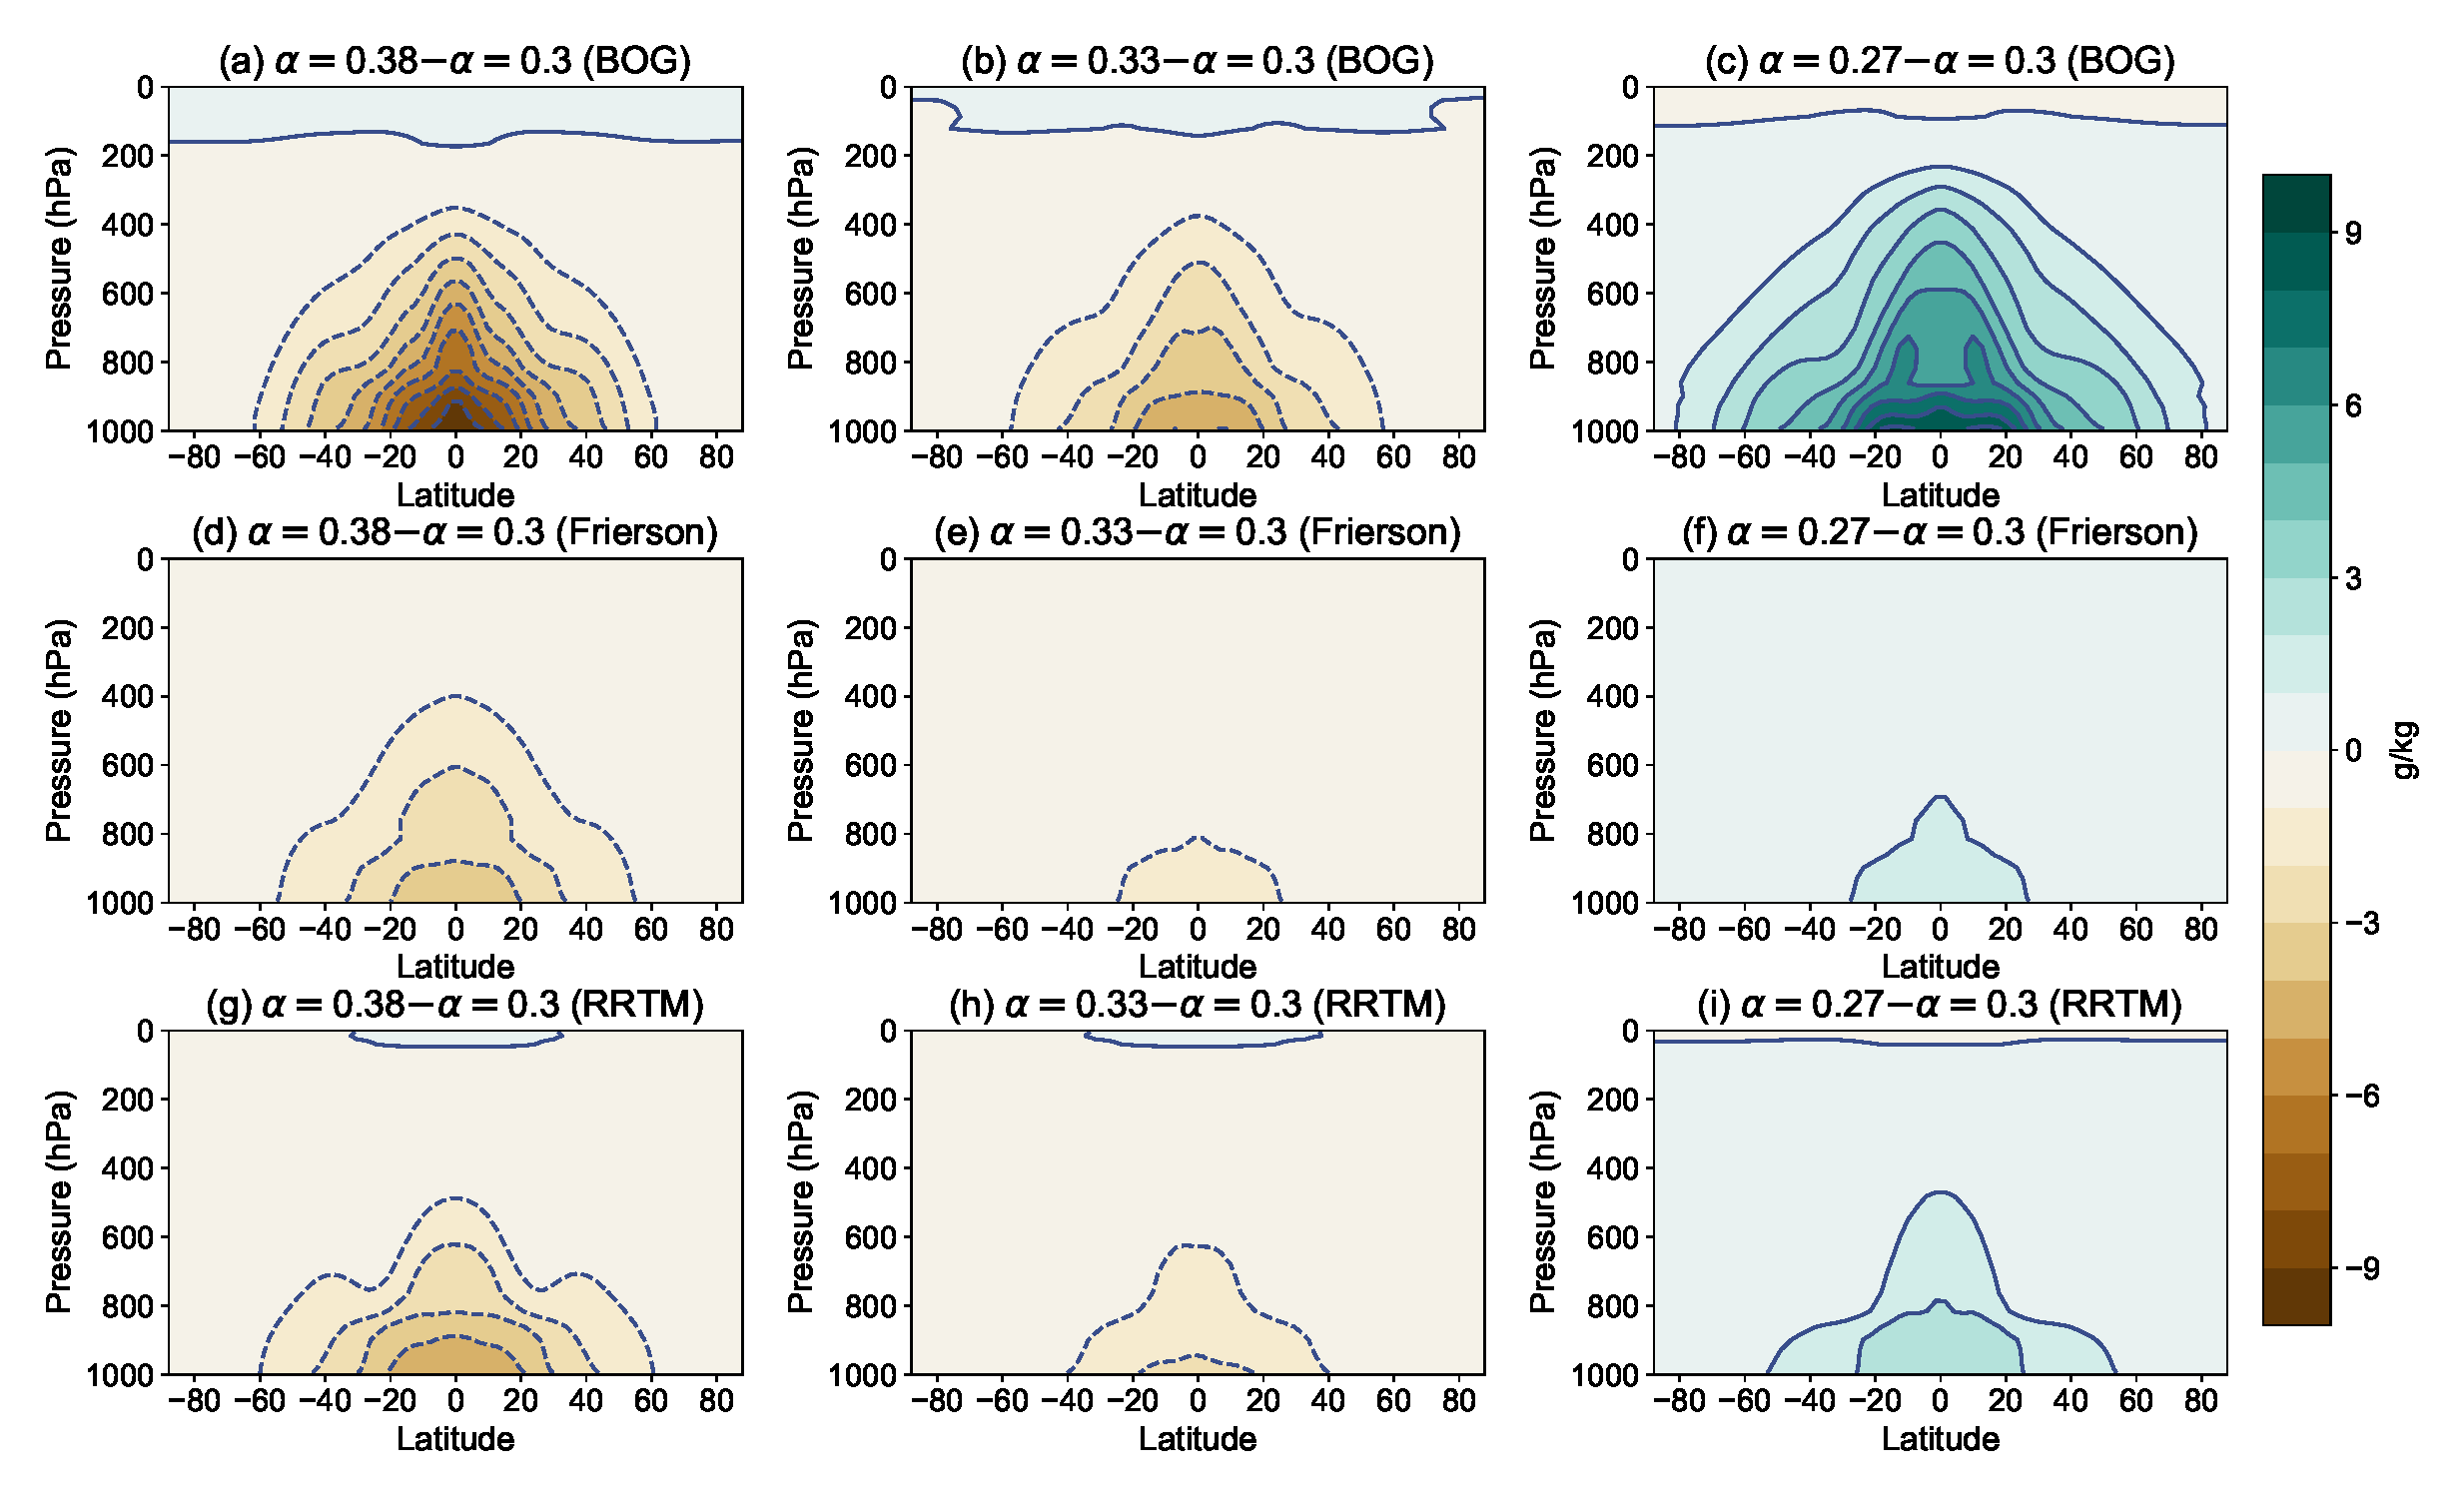
\includegraphics[width=1.0\linewidth]{figs/polar_amp/sphum_diff}
	\caption[The annual and zonal mean profiles of specific humidity changes]{As \figref{fig:vert_temp_diff}, but for the specific humidity change in experiments with BOG, Frierson and RRTM radiation schemes.}
	\label{fig:vert_q_diff}
\end{figure}

The annual and zonal mean change of moisture profiles from different radiation schemes are showed in \figref{fig:vert_q_diff}. It is clear that the change of specific humidity profile is strongest in BOG scheme and weakest in Frierson scheme, both in cooling and warming cases. Noting that the specific humidity increases (decreases) in warming (cooling) cases almost everywhere but most strongly near the surface at low latitudes, this indicates that the radiative effect of water vapor is strongly amplified at low latitudes \citep{Langen2012, Pithan2014}. However, the previous results show that even if the only difference between the BOG and Frierson radiation schemes lies in whether moisture feedback existing in longwave radiation transfer, the polar amplification of surface temperature change is evident in BOG scheme rather than in Frierson scheme (\figsref{fig:delta_ts} and \ref{fig:vert_temp_diff}), which implies that water vapor feedback is possibly associated with the contrast of surface temperature responses. As demonstrated in previous studies \citep[e.g.][]{Schneider1999}, the variability of clouds and water vapor fields are significant to the simulation of radiation field. It is for this reason that we perform the runs without moisture feedback in BOG scheme.
% Although there is a weak polar amplified effect in Frierson scheme

%which provide us a good chance to investigate the role of water vapor feedback in further. % suggesting that the radiation conditio
%is possible that the stark contrast between surface temperature responses in these two gray radiation schemes could be attributed to the distinct water vapor fields ().
%In our study, the reason why the responses from BOG and Frierson schemes are totally different
%and therefore we perform the experiments by reading the water vapor from control run into radiation schemes.

%As shown in previous sections, various aspects in BOG scheme, including the change of zonal mean surface temperature, the degree of polar amplification, and the northward heat transport, are all distinct from that from Frierson scheme and one possible reason is that moisture feedback exists in BOG scheme rather than Frierson scheme. 

\begin{figure}[ht]
	\centering
	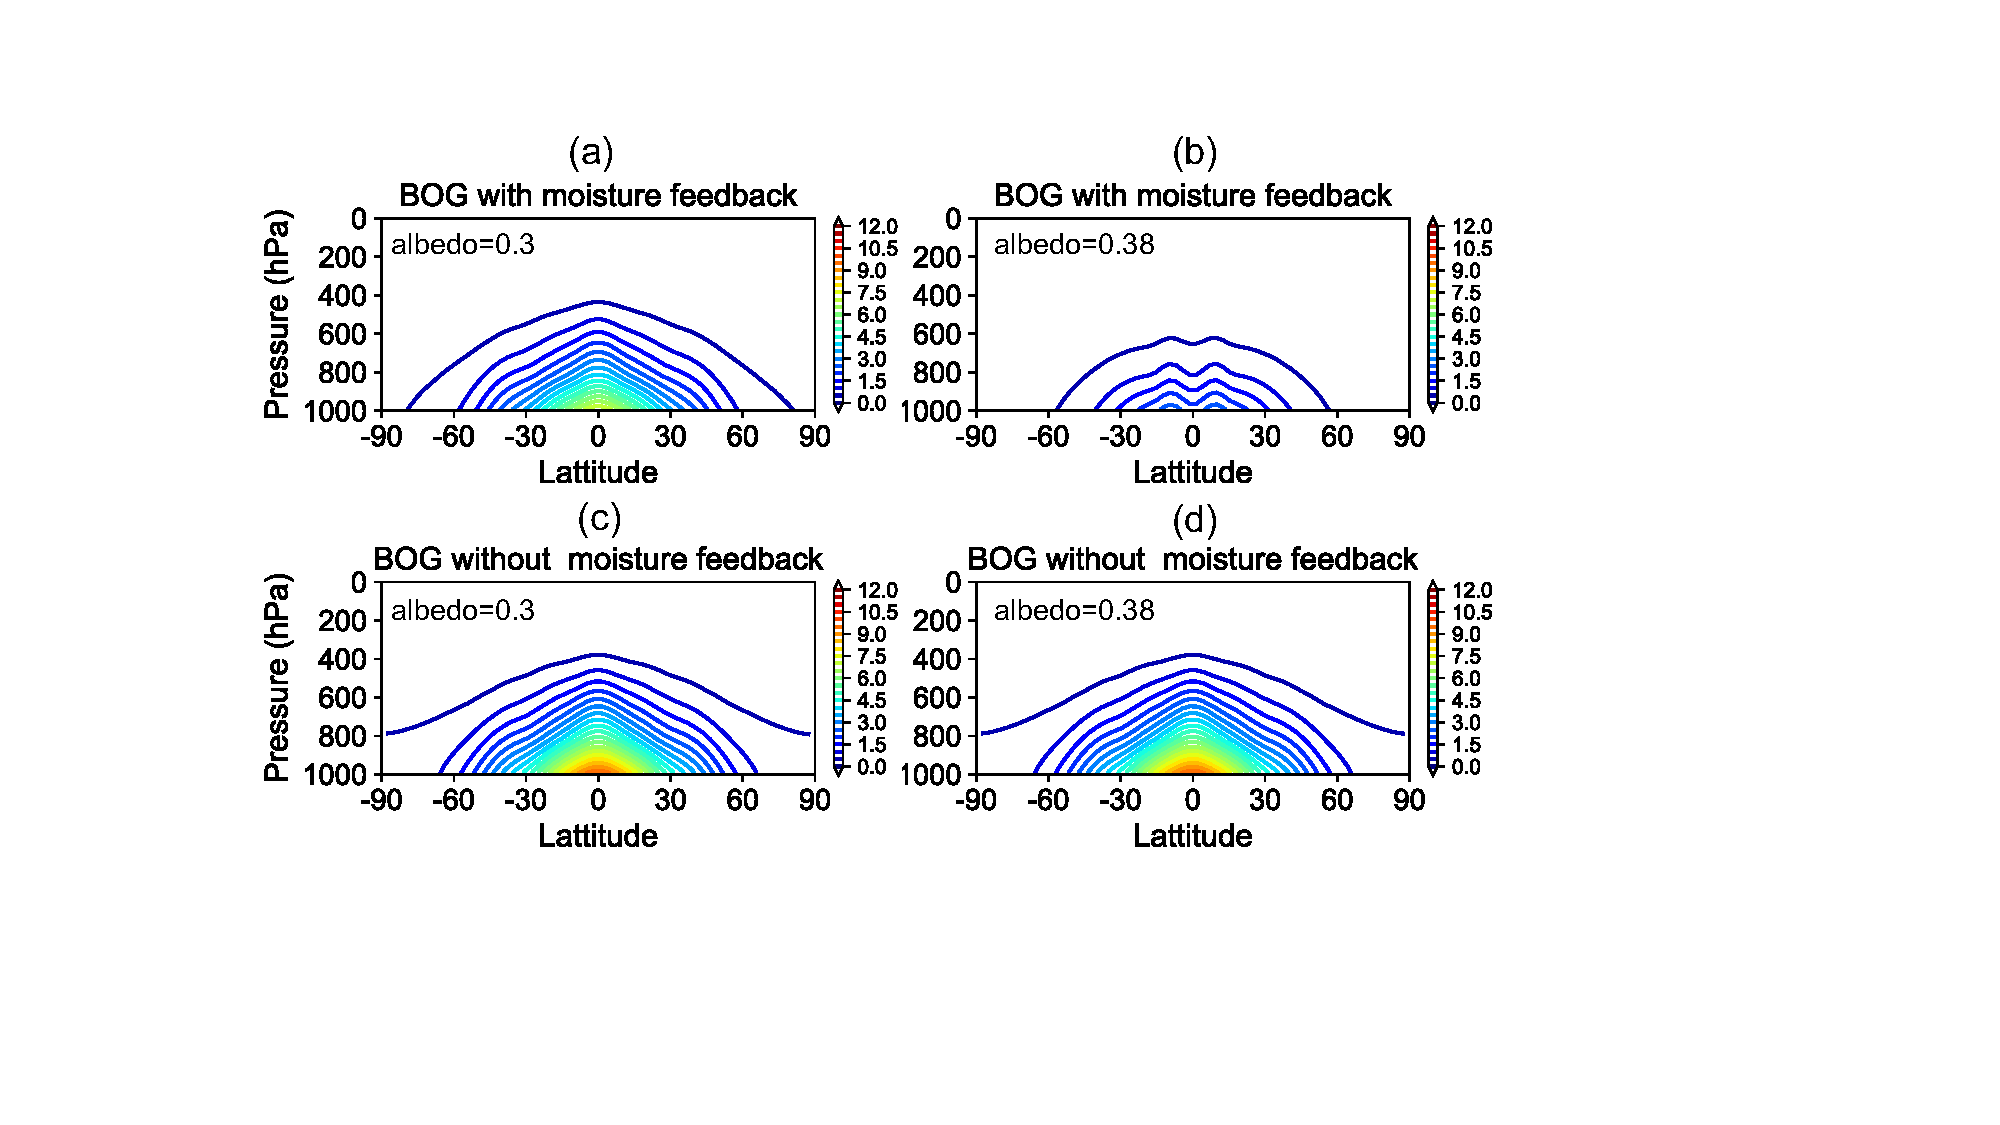
\includegraphics[width=0.8\textwidth]{{figs/polar_amp/lw_optical_depth}.pdf}
	\caption[Annual and zonal mean longwave optical depth in BOG radiation scheme before and after reading the $q$ profile.]{Annual and zonal mean longwave optical depth in BOG radiation scheme before and after reading the $q$ profile. (a) and (b) are the averaged longwave optical depth from the experiments with moisture feedback where albedo is 0.3 and 0.38. (c) and (d) are similar to (a) and (b), but the $q$ profiles are fixed by reading annual and zonal mean $q$ profile from control experiment (aledo is 0.3), so (c) and (d) are identical with each other.}
	\label{fig:optical_depth}
\end{figure}

To identify the role of moisture feedback in BOG radiation scheme, we read the specific humidity ($q$) profile from the control run (i.e. $\alpha=0.3$) into other experiments (i.e. $\alpha=0.38$, $0.33$ and $0.27$) to make the moisture feedback fixed in the longwave radiation transfer. The longwave optical depths are examined first before analyzing the simulation results. For instance, the original optical depth profiles from the two runs where albedos are 0.3 (\figref{fig:optical_depth}a) and 0.38 (\figref{fig:optical_depth}b) show great differences when the moisture feedback is freely performed in radiation schemes, but they are almost identical to each other after the specific humidity profile for the run where albedo is 0.38 has been specified by the profile from control experiment (\figref{fig:optical_depth}c and \ref{fig:optical_depth}d). Compared to the original optical depths, the runs with increased albedos (e.g. $\alpha=0.38$) have thicker optical depths as they have been prescribed with specific humidity profiles from a warmer control state ($\alpha=0.3$), where the atmospheric water vapor content is much larger due to the non-linear effect of saturation water vapor pressure with respect to temperature according to Clausius-Clapeyron relation. Similarly, the runs with decreased albedos will have a thinner optical depth as they are specified with moisture profiles from relative cold control state.

%Normally, temperature increases when albedo is changed from 0.38 to 0.3, and thus , meaning that the longwave optical depth becomes larger as albedo declines. In regard to the case where albedo is 0.3, the optical depth increasing slightly, which is normal because the water vapor content has to increase gradually with the temperature going up, but the moisture content is always high when the experiment is prescribed with the annually averaged specific humidity profile.
%as they are prescribed with the same specific humidity profile. 
%of experiment where albedo is 0.38 has been specified by the optical thickness from control experiment (\figref{fig:optical_depth}), where the optical depths in \figref{fig:optical_depth}c and \figref{fig:optical_depth}d are almost identical as they are prescribed with the same specific humidity profile. 
% SURFACE TEMPERATURE AND THIR CHANGE when no moisture feedback in BOG
% while the optical depth for control experiment doesn't change too much.

%\begin{table}[ht]
%	\centering
%	\caption{there is no moisture feedback in BOG radiation scheme.}
%	\begin{adjustbox}{center=\textwidth}
%		\begin{tabular}{l c c c}
%			\toprule
%			\multirow{2}{*}{Region} & \multicolumn{3}{c}{Byrne(albedo=$x$-ctrl)}  \\
%			\cline{2-4}  
%			& $x$=0.38 & $x$=0.33 & $x$=0.27\\
%			\midrule
%			Arctic & -5.62 & -2.23 & 2.03 \\
%			Globe & -4.64 & -1.71 & 1.67 \\
%			$\Delta T_A/\Delta T_G$ & 1.21 & 1.31 & 1.22\\
%			\bottomrule
%		\end{tabular}
%	\end{adjustbox}
%	\label{tab:arctic_global_warming_ratio_no_wv}
%\end{table}

The surface temperature change for BOG radiation scheme without moisture feedback (BOG-qctrl, orange dash-dotted lines in \figref{fig:delta_ts}) shows different behaviors from the runs with water vapor feedback, where the zonal mean surface temperature changes are much smaller and polar amplification becomes much weaker compared to the original runs. This indicates that the moisture feedback plays an important role in the surface temperature change as well as polar amplification at least in BOG scheme. Note that the surface temperature changes in the runs without moisture feedback in BOG scheme are close to those in Frierson scheme, which is reasonable as the moisture feedback is also missing in Frierson scheme. In addition, the vertical temperature profiles in polar and tropical regions also change a lot when there is no water vapor feedback in BOG scheme. Specifically, the bottom-heavy cooling or warming profiles become less evident in polar region (see the orange dash-dotted lines in \figsref{fig:delta_t_profile}a-c) and the top-heavy cooling or warming profiles get weaker in tropical region (orange dash-dotted lines in \figsref{fig:delta_t_profile}d-f), implying the positive lapse rate feedback is weakened in polar region.

%To find out the outcome in BOG radaition scheme without moisture feedback, we turn to the changes of surface temperature with various albedos. As shown in \tabref{tab:arctic_global_warming_ratio_no_wv}, the changes of Arctic and global mean surface temperature when changing albedos have decreased drastically compared to the ones in experiments with allowing moisture feedback. In addition, the polar amplification of surface temperature in BOG scheme without moisture feedback is no longer evident, and the ratios of surface temperature changes in Arctic and globe become close to the ones from Frierson scheme (shown in \tabref{tab:arctic_global_warming_ratio}). 

%Whta's more, the northward heat transports resemble to each other (\figref{fig:ht_bog_no_wv_fb}) and the abnormal behaviours, such as reversals in latent heat transport and Hadley cell circulation (\figref{fig:hadleycell_no_moisture}), in the experiment where albedo is 0.38 also disappear when there is no moisture feedback in BOG radiation scheme. All the facts above indicate that the moisture feedback plays an important role in the change of surface temperature as well as polar amplification when adopting different albedos in BOG scheme. 

%\begin{figure}[ht]
%	\centering
%	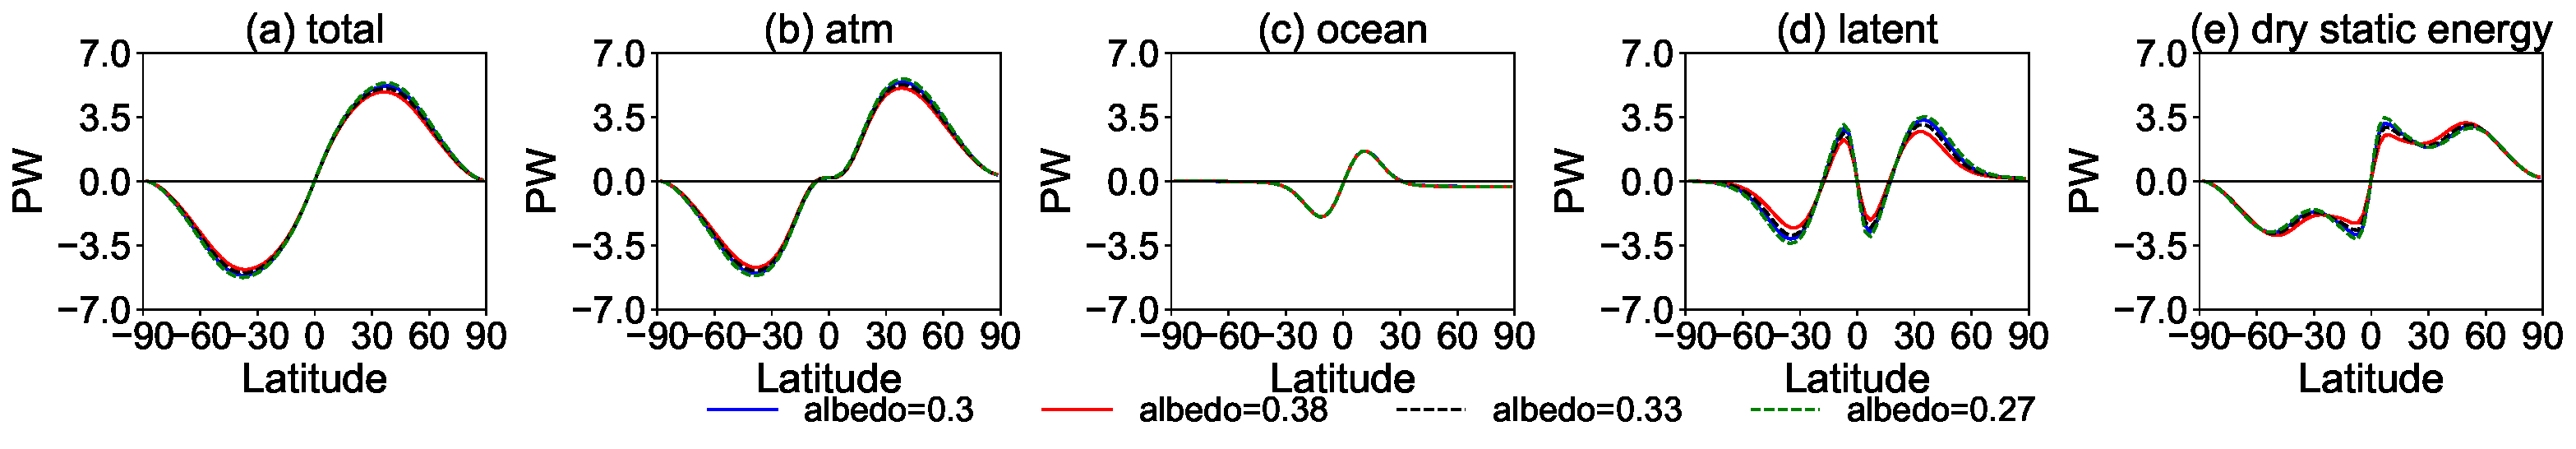
\includegraphics[width=1.0\textwidth]{figs/polar_amp/ht_bog_no_moisture.pdf}
%	\caption{As the transport for BOG scheme in \figref{fig:ht_transport}, but no moisture feedback there.}
%	\label{fig:ht_bog_no_wv_fb}
%\end{figure}
%
%\begin{figure}[ht]
%	\centering
%	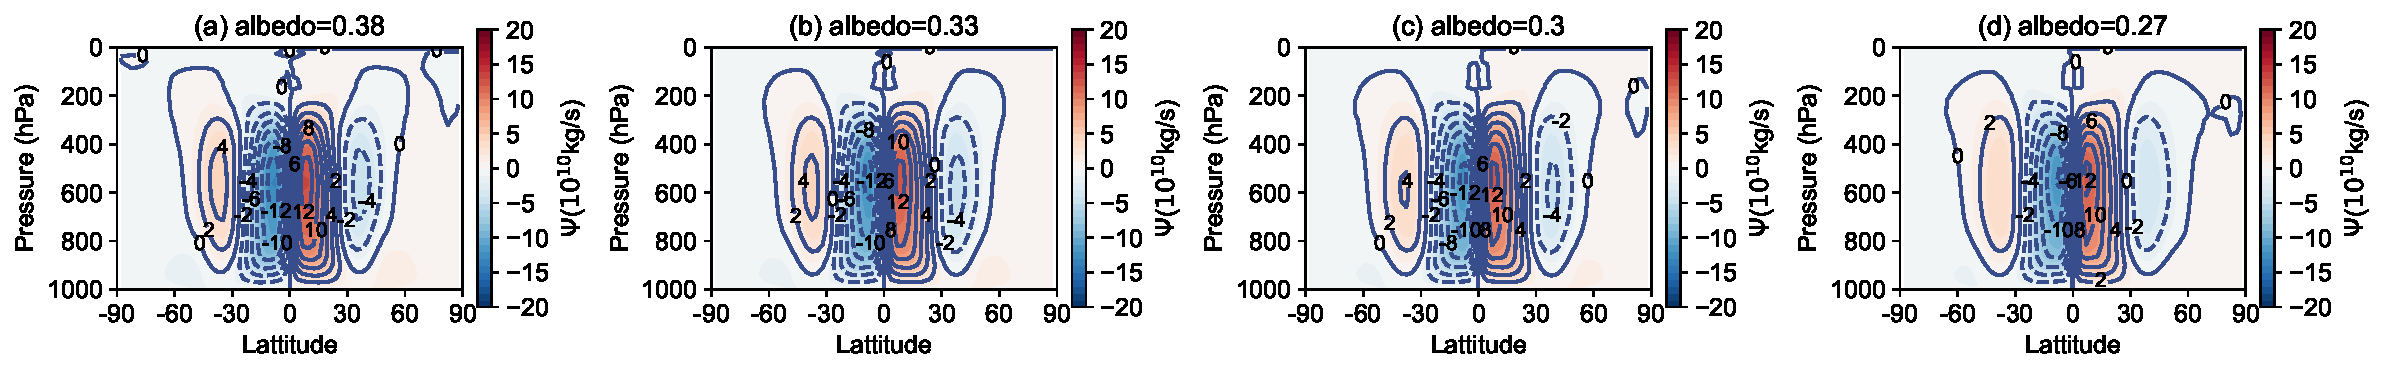
\includegraphics[width=1.0\textwidth]{figs/polar_amp/compare_bog_moisture_feedback/hadley_cell_bog_without_moisture_feedback.pdf}
%	\caption{As in \figref{fig:haleycell_bog}, but there is no moisture feedback in BOG radiation scheme.}
%	\label{fig:hadleycell_no_moisture}
%\end{figure}
%
%However, there is still slight polar amplification even when there is no moisture feedback in BOG radiation scheme when changing albedos as shown by $\Delta T_A/\Delta T_G$ in \tabref{tab:arctic_global_warming_ratio_no_wv}. Recall that the relationship between northward heat transport and surface temperature changes in Arctic and global areas has been discussed in \secref{sec:ht_hadley}, here the linkage is affirmed again. \figref{fig:ht_diff_bog_no_wv_fb} displays the differences of heat transport when changing albedos in BOG radiation scheme without moisture feedback. Similarly, the differences of regional mean surface temperature both in Arctic and globe are approximately proportional to the differences of maximum of northward latent heat transport (\figref{fig:deltaT_lht_no_wv_fb}), which can be used to explain the slight polar amplification when changing albedos in BOG radiation scheme even without moisture feedback.
%
%\begin{figure}[ht]
%	\centering
%	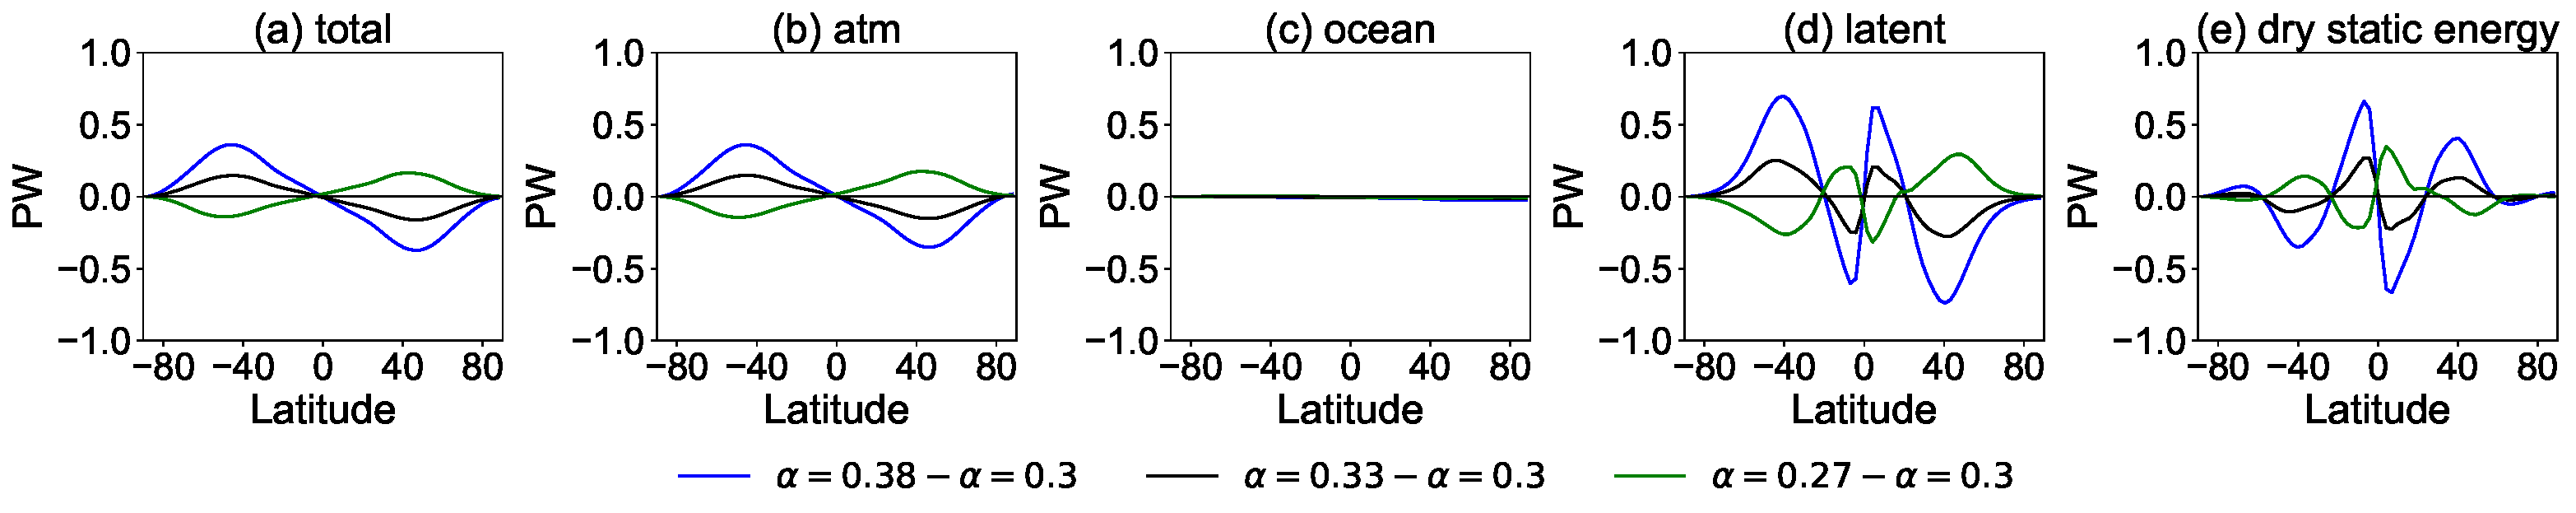
\includegraphics[width=1.0\textwidth]{figs/polar_amp/compare_bog_moisture_feedback/ht_diff_bog_no_moisture.pdf}
%	\caption{As the difference of heat transport for BOG scheme in \figref{fig:ht_transport_diff}, but no moisture feedback in these experiments.}
%	\label{fig:ht_diff_bog_no_wv_fb}
%\end{figure}
%
%\begin{figure}[ht]
%	\centering
%	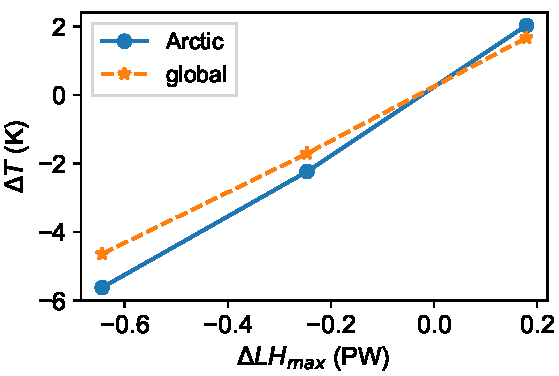
\includegraphics[width=0.5\textwidth]{figs/polar_amp/linear_relation_Delta_T_ht_no_moisture_bog.pdf}
%	\caption{The relationship between the differences of regional mean surface temperature and the differences of maximum of northward latent heat transport in BOG radiation scheme without moisture feedback.}
%	\label{fig:deltaT_lht_no_wv_fb}
%\end{figure}
%

\begin{figure}[ht]
	\centering
	\makebox[\linewidth]{
	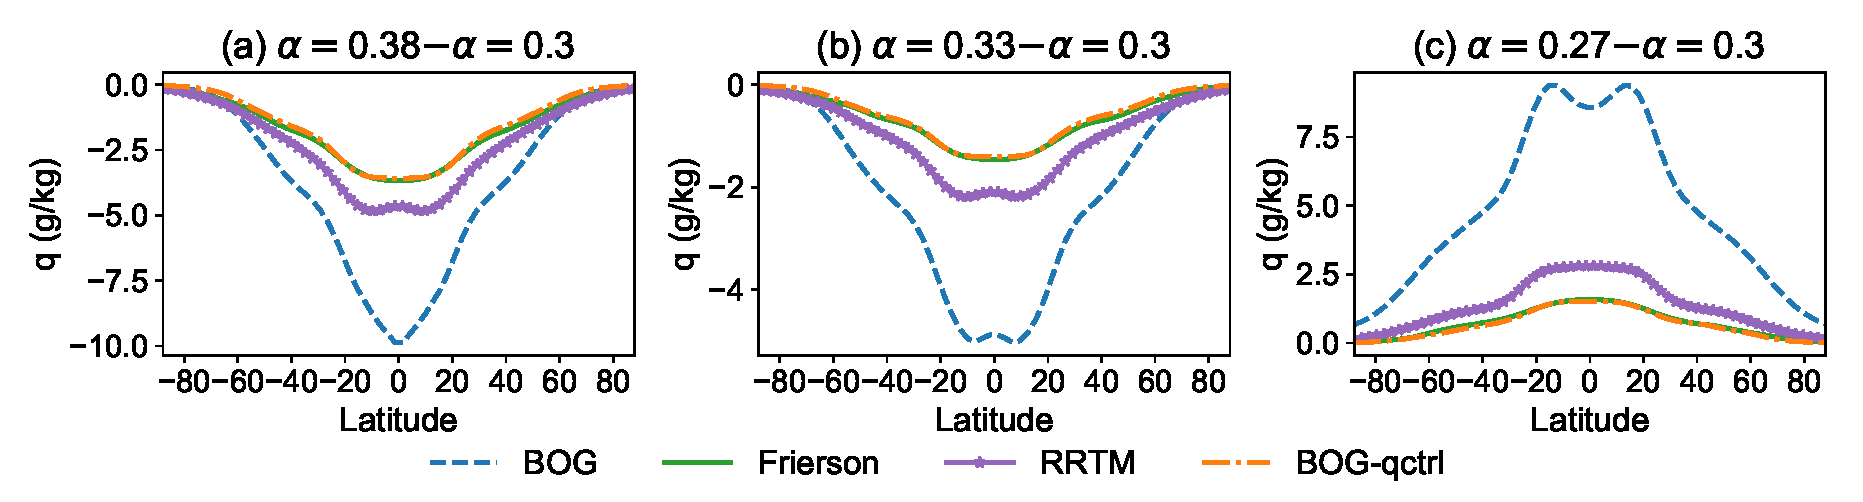
\includegraphics[width=1.1\textwidth]{figs/polar_amp/sfc_q_diff_gradient}}
	\caption[The zonal and annual mean specific humidity changes]{As in \figref{fig:delta_ts}, but for the specific humidity at surface. }
	\label{fig:sfc_q_zonal}
\end{figure}

As remarked by \cite{Pithan2014}, the water vapor feedback contributes more to the tropical warming than to polar warming, which corresponds to our findings for BOG radiation scheme (\secref{sec:climate_feedbacks_temp_decomp}). But we should also notice that while water vapor feedback does not result in polar amplification by itself, it could approximately double the climate sensitivity both at low and high latitudes \citep{Langen2012}. However, we find the polar amplification of surface temperature decreases remarkably after turning off the water vapor feedback, which as illustrated in \figref{fig:sfc_q_zonal} (blue dashed and orange dash-dotted lines). This is due to the water vapor content and its meridional gradient, which have both changed when the moisture feedback is turned off. In addition, the zonal mean profile from BOG scheme with moisture feedback is quite different from RRTM scheme, suggesting that the moisture feedback prescribed in BOG radiation scheme is possibly too strong compared to a more realistic radiation scheme. Although the water vapor is only specified in radiation code, other processes associated with the advection and latent heat release are still retained in BOG experiment, that is why the runs without moisture feedback (BOG-qctrl) behave so similarly to Frierson scheme. As illustrated in \figref{fig:tsurf_diff}, there is still slight amplified surface temperature change at high latitudes even if no moisture feedback is included in radiation schemes, and therefore other mechanisms need to be investigated.

% However, it is the unreasonable meridional water vapor gradient from tropics to pole that amplify the surface temperature change in high latitudes.

%But we found at least in BOG radiation scheme, the moisture feedback plays a significant role in the surface temperature changes, where the polar amplification decreases largely without moisture feedback, which gives the causes to the differences between BOG and Frierson radiation scheme. In addition, there is 

%% --------------- Heat Transport ----------------- %%
\subsection{Heat transport}
\label{sec:heat_transport}

%The heat transports in all experiments will be analyzed to discern the roles of different components.
%For instance, considering the difference in BOG and Frierson radiation schemes, the latent heat transport will be focused on in particular as water vapor is related to the latent heat release. 
 
The total northward energy transport $H$ across each latitude ($\varphi$) is calculated by the energy budget balance in an atmospheric column,
\begin{equation}
	H(\varphi) =  \int_{-\frac{\pi}{2}}^{\varphi}2\pi a^2(ASR-OLR)\operatorname{cos}\varphi \operatorname{d}\varphi,
\end{equation}  
where $a$ is the radius of Earth, $ASR$ is the absorbed solar radiation flux and $OLR$ is outward longwave radiation flux at latitude band, and hence $ASR-OLR$ is the net TOA radiation. The total northward energy transport can be decomposed into energy transport by atmosphere and ocean. In our aquaplanet experiments, there is no Q-flux to represent the ocean heat transport, so the total energy transport is contributed from atmospheric energy transport ($H_{a}$, AET) only:
\begin{equation}
	H_a(\varphi) = H(\varphi).
\end{equation}
%In our aquaplanet experiments, a Q-flux is added as the oceanic heat transport, which is the same in all experiments and thus has no effect to the temperature responses after changing abledos. 

%Therefore, the northward oceanic energy transport $H_o$ is
%\begin{equation}
%H_o(\varphi)= -2\pi a^2\int_{-\frac{\pi}{2}}^{\varphi}\operatorname{cos}\varphi F_s\operatorname{d}\varphi,
%\end{equation}  and atmospheric energy transport $H_a$ is 
%\begin{equation}
%	H_a(\varphi)= 2\pi a^2\int_{-\frac{\pi}{2}}^{\varphi}\operatorname{cos}\varphi  (ASR-OLR+F_s)\operatorname{d}\varphi,
%\end{equation}  
%where $F_s$ represents the surface energy budget and is given by 
%\begin{equation}
%	Fs=SW+LW-SH-LH+\nabla \cdot \bm Q,
%\end{equation}
%in which $SW$ and $LW$ are the net shortwave and longwave radiation flux at surface, $SH$ is the sensible heat flux, $LH$ is the latent heat flux and $\bm Q$ is the Q-flux. 
In addition, the northward AET can be decomposed in further into latent heat transport ($H_{LH}$), which is related to latent heat release, and dry static energy transport ($H_{dry}$) associated with the motion of dry air, which are given by 
\begin{equation}
	H_{LH}(\varphi)= 2\pi a^2\int_{-\frac{\pi}{2}}^{\varphi}\operatorname{cos}\varphi  L_v(E-P)\operatorname{d}\varphi,
\end{equation}
and 
\begin{equation}
H_{dry}=H_a-H_{LH},
\end{equation}
where $E$ and $P$ denote evaporation and precipitation respectively, and $L_v$ is the specific latent heat capacity. The meridional energy transports mentioned above in all experiments for BOG, Frierson and RRTM radiation schemes are shown in the \figref{fig:ht_transport} and the changes of energy transport after changing albedos are displayed in \figref{fig:ht_transport_diff}.

\begin{figure}[ht]
	\centering
	\makebox[\linewidth]{
	%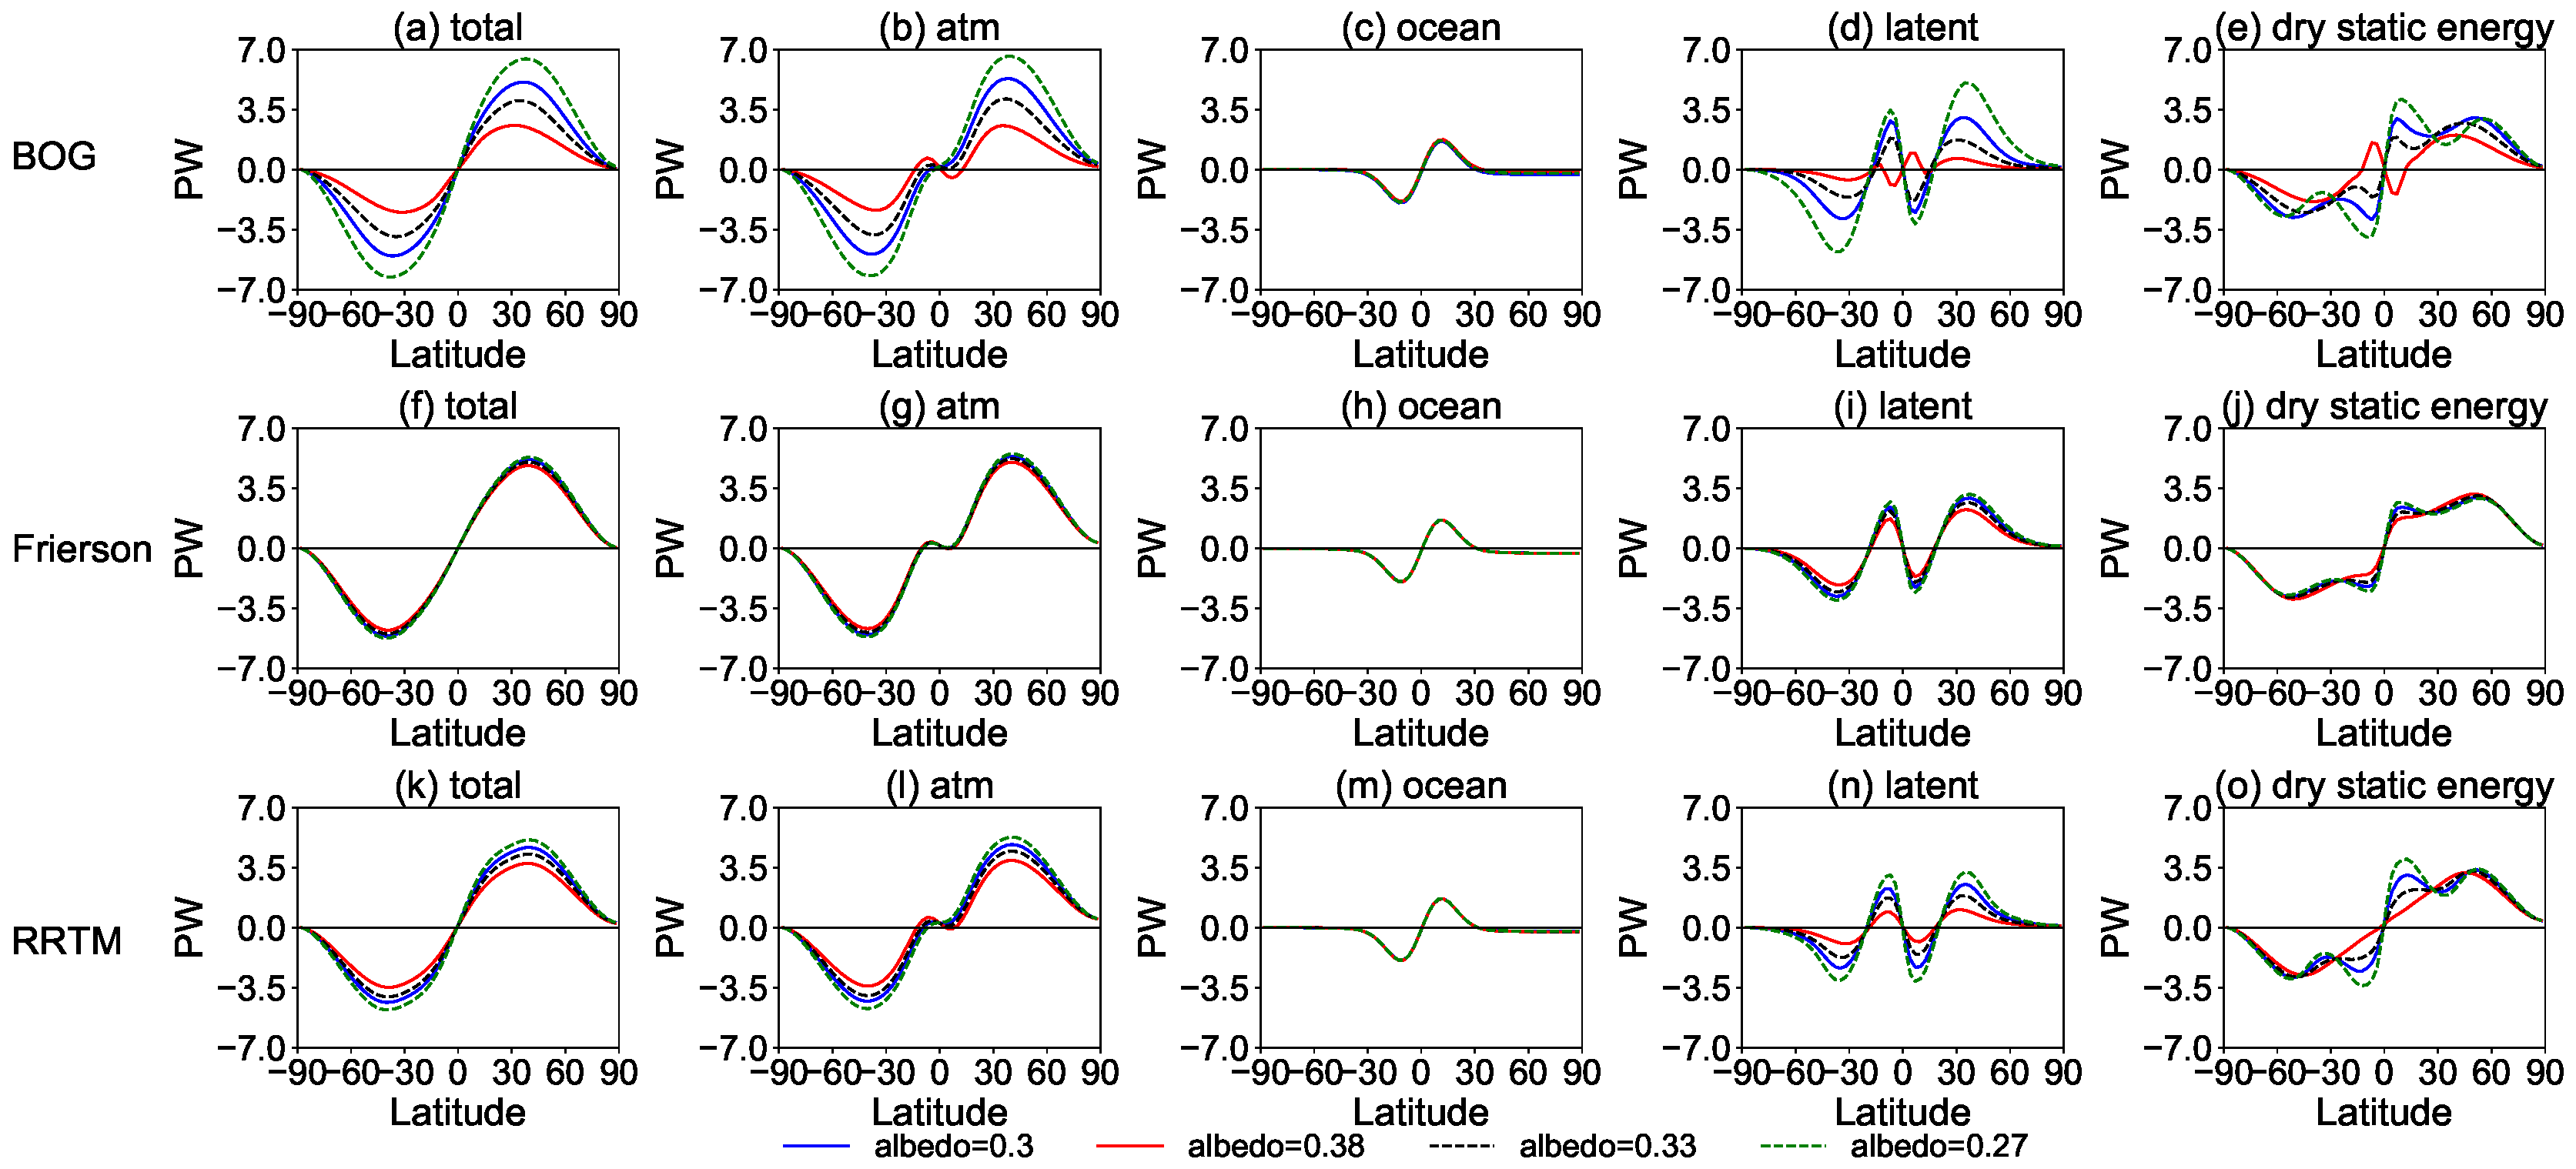
\includegraphics[width=1.1\linewidth]{{figs/polar_amp/poleward_ht_diff_compnts_diff_schemes_0.3_0.38_0.33_0.27}.pdf}}
	% \caption{Heat transport in the experiments with different radiation schemes and various albedos. The top, middle and bottom panels are for the BOG, Frierson and RRTM radiation schemes respectively. Total northward heat transports are shown in (a), (f) and (k), the atmospheric heat transports are presented in (b), (g) and (l), the oceanic heat transport related to Q-flux are listed in (c), (h) and (m), the latent heat transport are illustrated in (d), (i) and (n), and the dry static energy transport are depicted in (e), (j) and (o). Blue solid, red solid, blue dash and green dash lines indicate the experiments where albedos are 0.3, 0.38, 0.33 and 0.27 respectively.}
	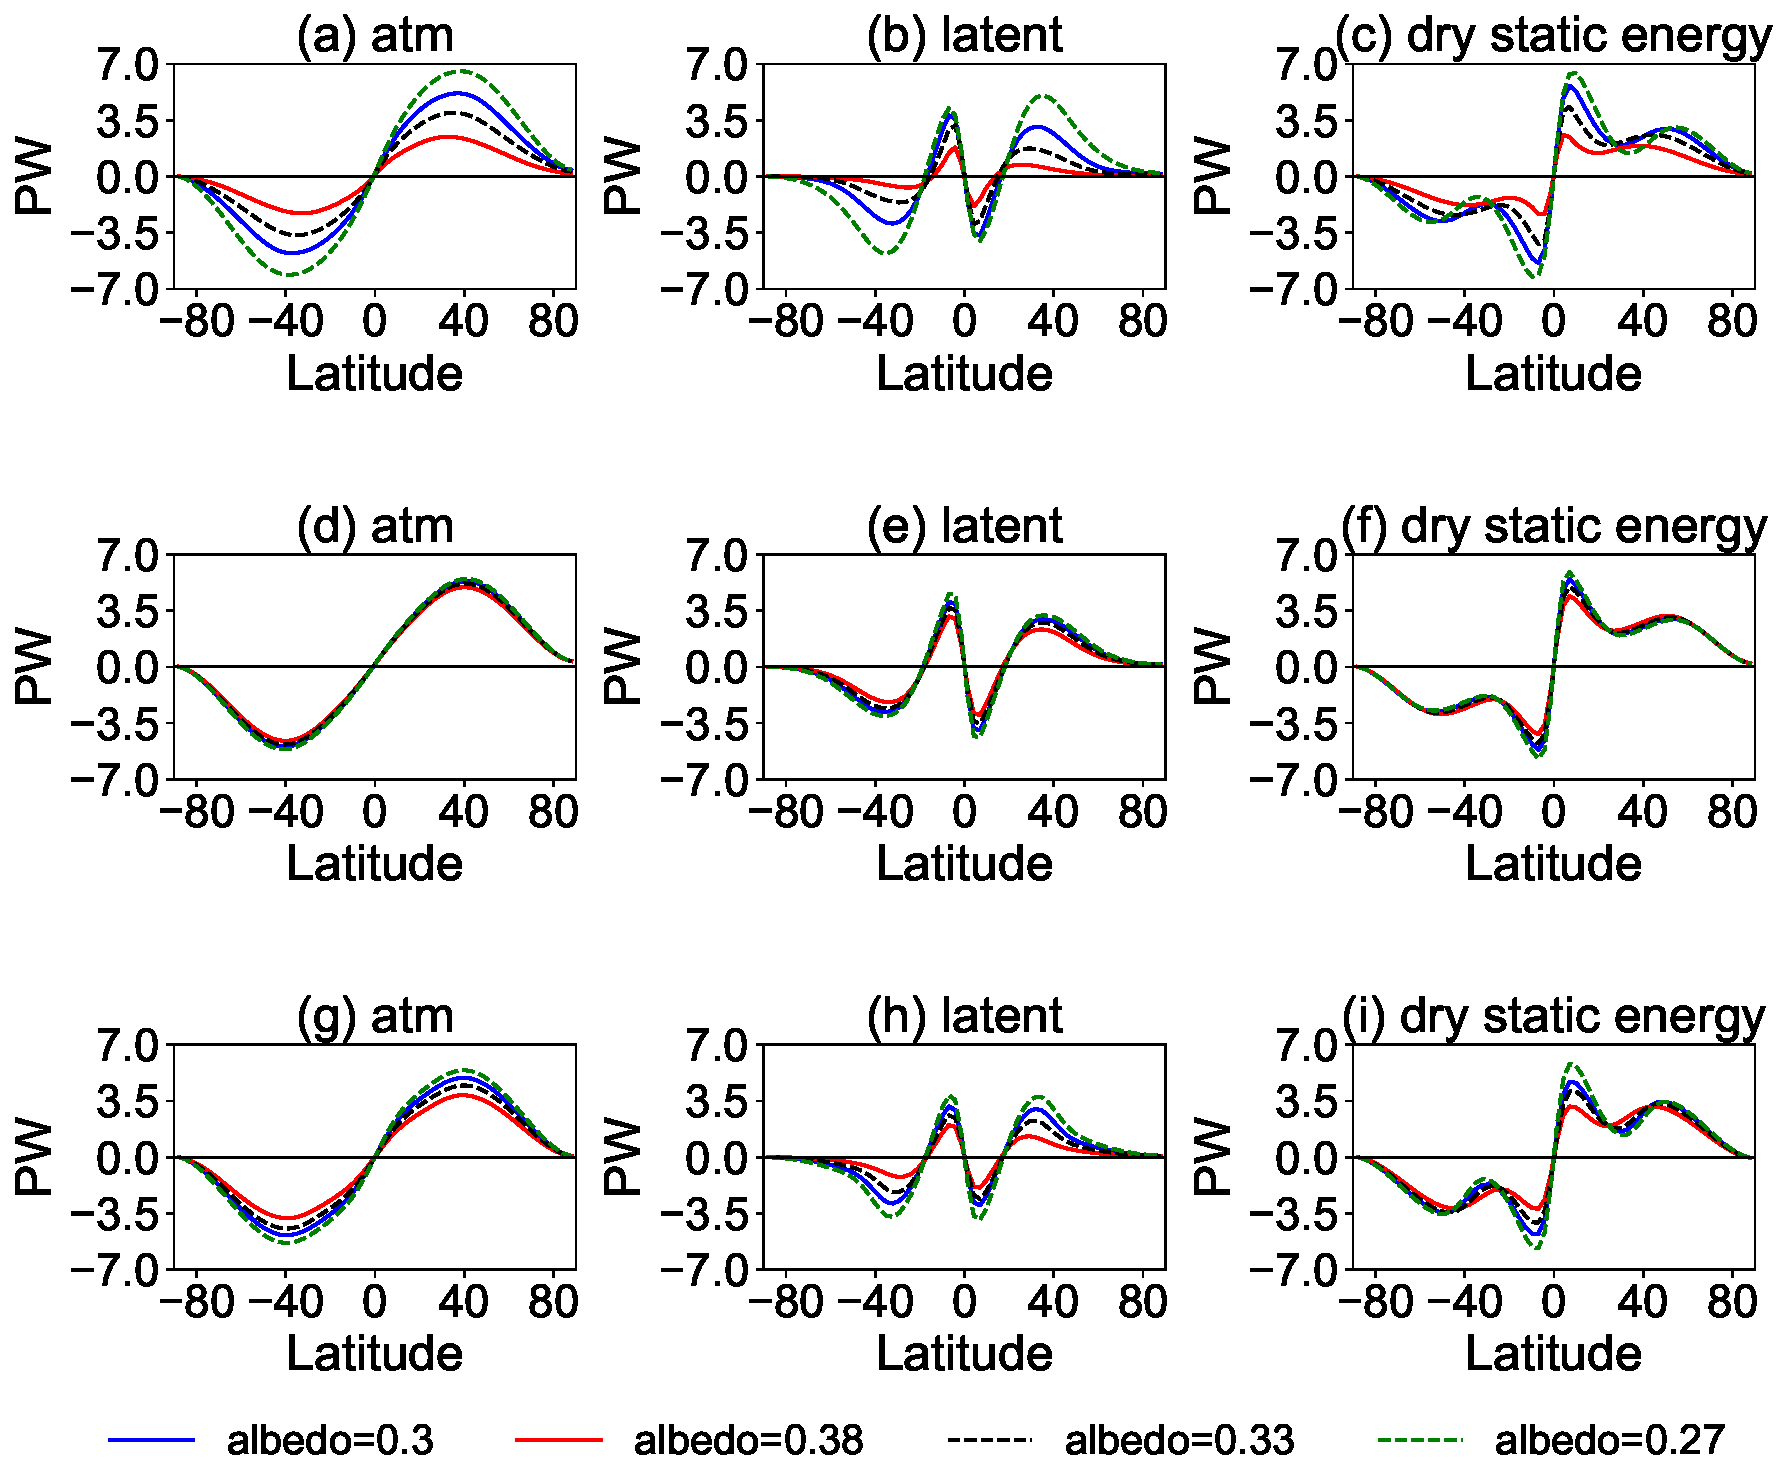
\includegraphics[width=0.9\linewidth]{{figs/polar_amp/poleward_ht_diff_compnts_diff_schemes}.pdf}}
    \caption[Heat transport in the experiments with different radiation schemes and various albedos]{Heat transport in the experiments with different radiation schemes and various albedos. The top, middle and bottom panels are for the BOG, Frierson and RRTM radiation schemes respectively. The atmospheric heat transports are presented in (a), (d) and (g), the latent heat transport are illustrated in (b), (e) and (h), and the dry static energy transport are depicted in (c), (f) and (i). Blue solid, red solid, blue dash and green dash lines indicate the experiments where albedos are 0.3, 0.38, 0.33 and 0.27 respectively.}
	\label{fig:ht_transport}
\end{figure}

%$$\frac{\partial E_o}{\partial t} = -F_s- \frac{1}{2\pi a^2\operatorname{cos}\varphi}\frac{\partial H_o(\varphi)}{\partial \varphi}$$
%$$\frac{\partial E_a}{\partial t} = R_{TOA}+F_s- \frac{1}{2\pi a^2\operatorname{cos}\varphi}\frac{\partial H_a(\varphi)}{\partial \varphi}$$
%$$L_v\frac{\partial Q}{\partial t} = L_v(Evap-Precip)- \frac{1}{2\pi a^2\operatorname{cos}\varphi}\frac{\partial H_{LH}(\varphi)}{\partial \varphi}$$

%For the simulations with BOG's radiation scheme, the TET shows large differences between the runs where the albedos are 0.38 and 0.3. The TET is composed of atmospheric and oceanic energy transport, and the oceanic energy transports are nearly the same (\figref{fig:ht_transport}c), so the main differences of TET are from the atmospheric energy transport (\figref{fig:ht_transport}b), most of which are contributed from latent heat transport (\figref{fig:ht_transport}d). However, all the energy transport for the simulations with Frierson's scheme are almost equal when changing the albedos, indicating that it is the moisture in the radiation scheme that leads to the polar amplification in the experiments with BOG's radiation scheme.


% In the aquaplanet setups, the mixed layer is prescribed with same Q-flux symmetric to the equator in the experiments, and thus the northward ocean heat transports in all experiments resemble to each other (\figsref{fig:ht_transport}c, h, m) and the differences when changing the albedos are nearly zero (\figsref{fig:ht_transport_diff}c, h, m). Therefore, the difference in total energy transport are from the atmospheric sources rather than from oceanic ones. 

The changes of the surface albedo do have influence on the atmopspheric energy transports in these experiments, although the degree of influence is different. The experiments performed with BOG radiation scheme have the largest changes after varying the albedo, the runs with RRTM radiation schemes have moderate changes, while the ones with Frierson schemes have the least effect (\figsref{fig:ht_transport}a, d and g), which are much clearer when checking the differences of the experiments in \figsref{fig:ht_transport_diff}. Compared to the dry static energy transport, the latent heat transport contributes a larger portion to the total atmospheric at 40$^\circ$ poleward (\figsref{fig:ht_transport} and \ref{fig:ht_transport_diff}). Previous studies have shown that an increase in atmospheric heat transport can cause midtropospheric warming in polar region \citep[e.g.,][]{Screen2012}, which can explain indirectly the polar amplification in experiments under seasonal or annual mean insolations \citep{Kim2018}.  Here we also examined the temperature change in polar region ($70^\circ$ northward) both at surface and mid-troposphere (450-700hPa) (\figref{fig:delta_ht_ts}). The results show strong linear relationships between the total AET change across $70^\circ$ and either the surface temperature change and ($R^2=0.97$, \figref{fig:delta_ht_ts}a) or mid-troposphere temperature change ($R^2=0.90$, \figref{fig:delta_ht_ts}b), implying that the heat transport is associated with the polar amplification both at surface and mid-troposphere under insolation conditions.

% The results show strong linear relationships between the surface temperature change and the total AET change across $70^\circ$ ($R^2=0.98$, \figref{fig:delta_ht_ts}a) and between mid-troposphere temperature change and poleward AET at $70^\circ$ ($R^2=0.93$, \figref{fig:delta_ht_ts}b), implying that the heat transport is much possible associated with the polar amplification at surface.

%\cite{Feldl2017}
%because in the two cases the polar warming is largest in mid-troposphere rather than at surface.

%Furthermore, the differences of total or latent heat transport are largest in BOG scheme, moderate in RRTM scheme and least in Frierson scheme, which seems to explain the varying levels of polar amplification in the three radiation schemes. In order to link the surface temperature change and polar amplification with the latent heat transport, the change of surface temperature after increasing or decreasing albedos are compared with the difference of maximum of northward latent heat transport, used as a proxy to represent the change of northward latent heat transport, in all the three radiations (\figref{fig:delta_ht_ts}). Strikingly, both the changes of Arctic and global mean of surface temperature due to various albedos have good linear relationships with changes of maximum of latent heat transport for all three radiation schemes, indicating that the changes of latent heat transport may explain the differences of global mean surface temperature as well as the polar amplification.

\begin{figure}[ht]
	\centering
	%\hspace{-1cm}
	%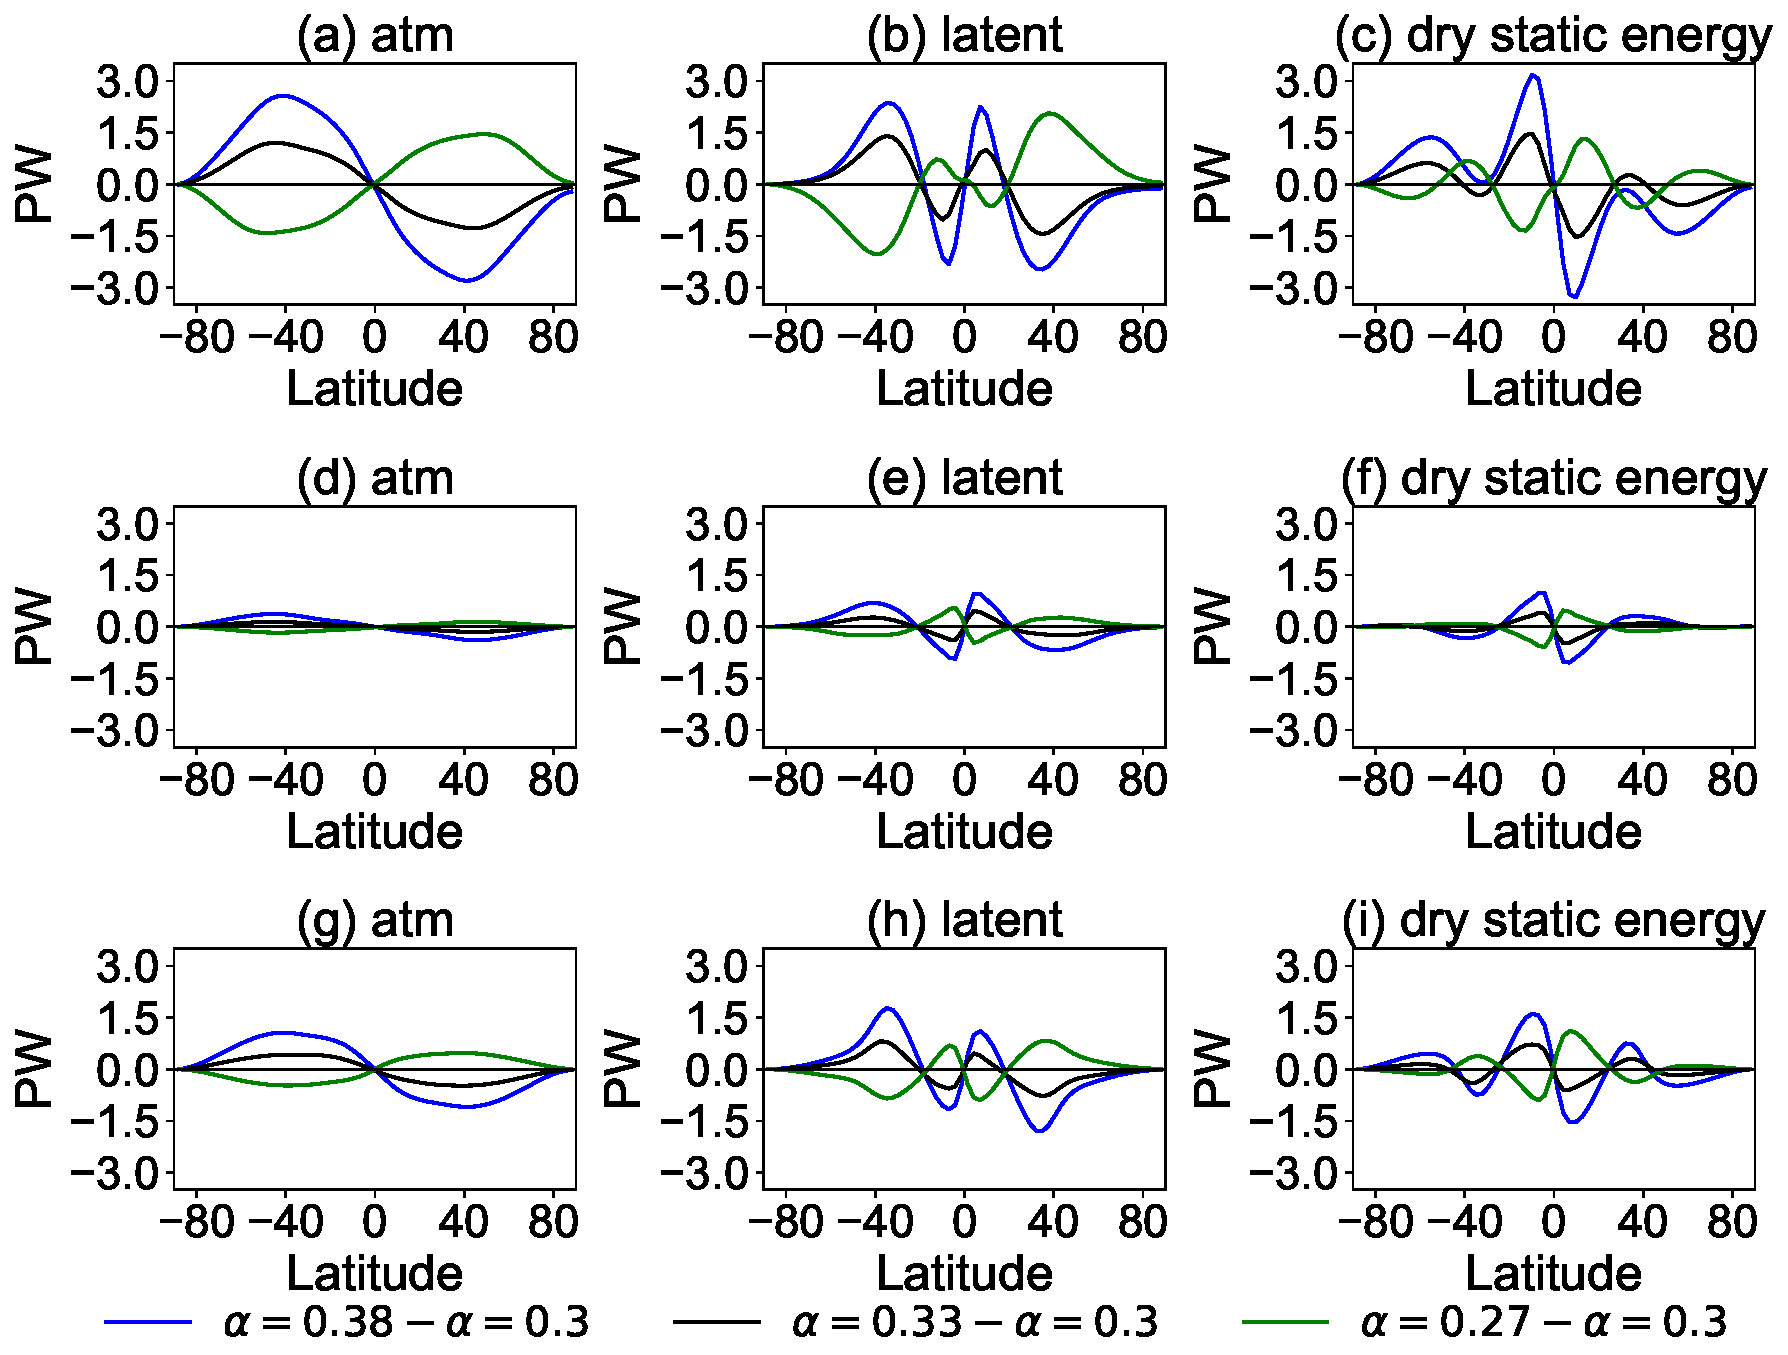
\includegraphics[width=1.\linewidth]{{figs/polar_amp/heat_transport_bog_frierson_components_diff_test}.pdf}
	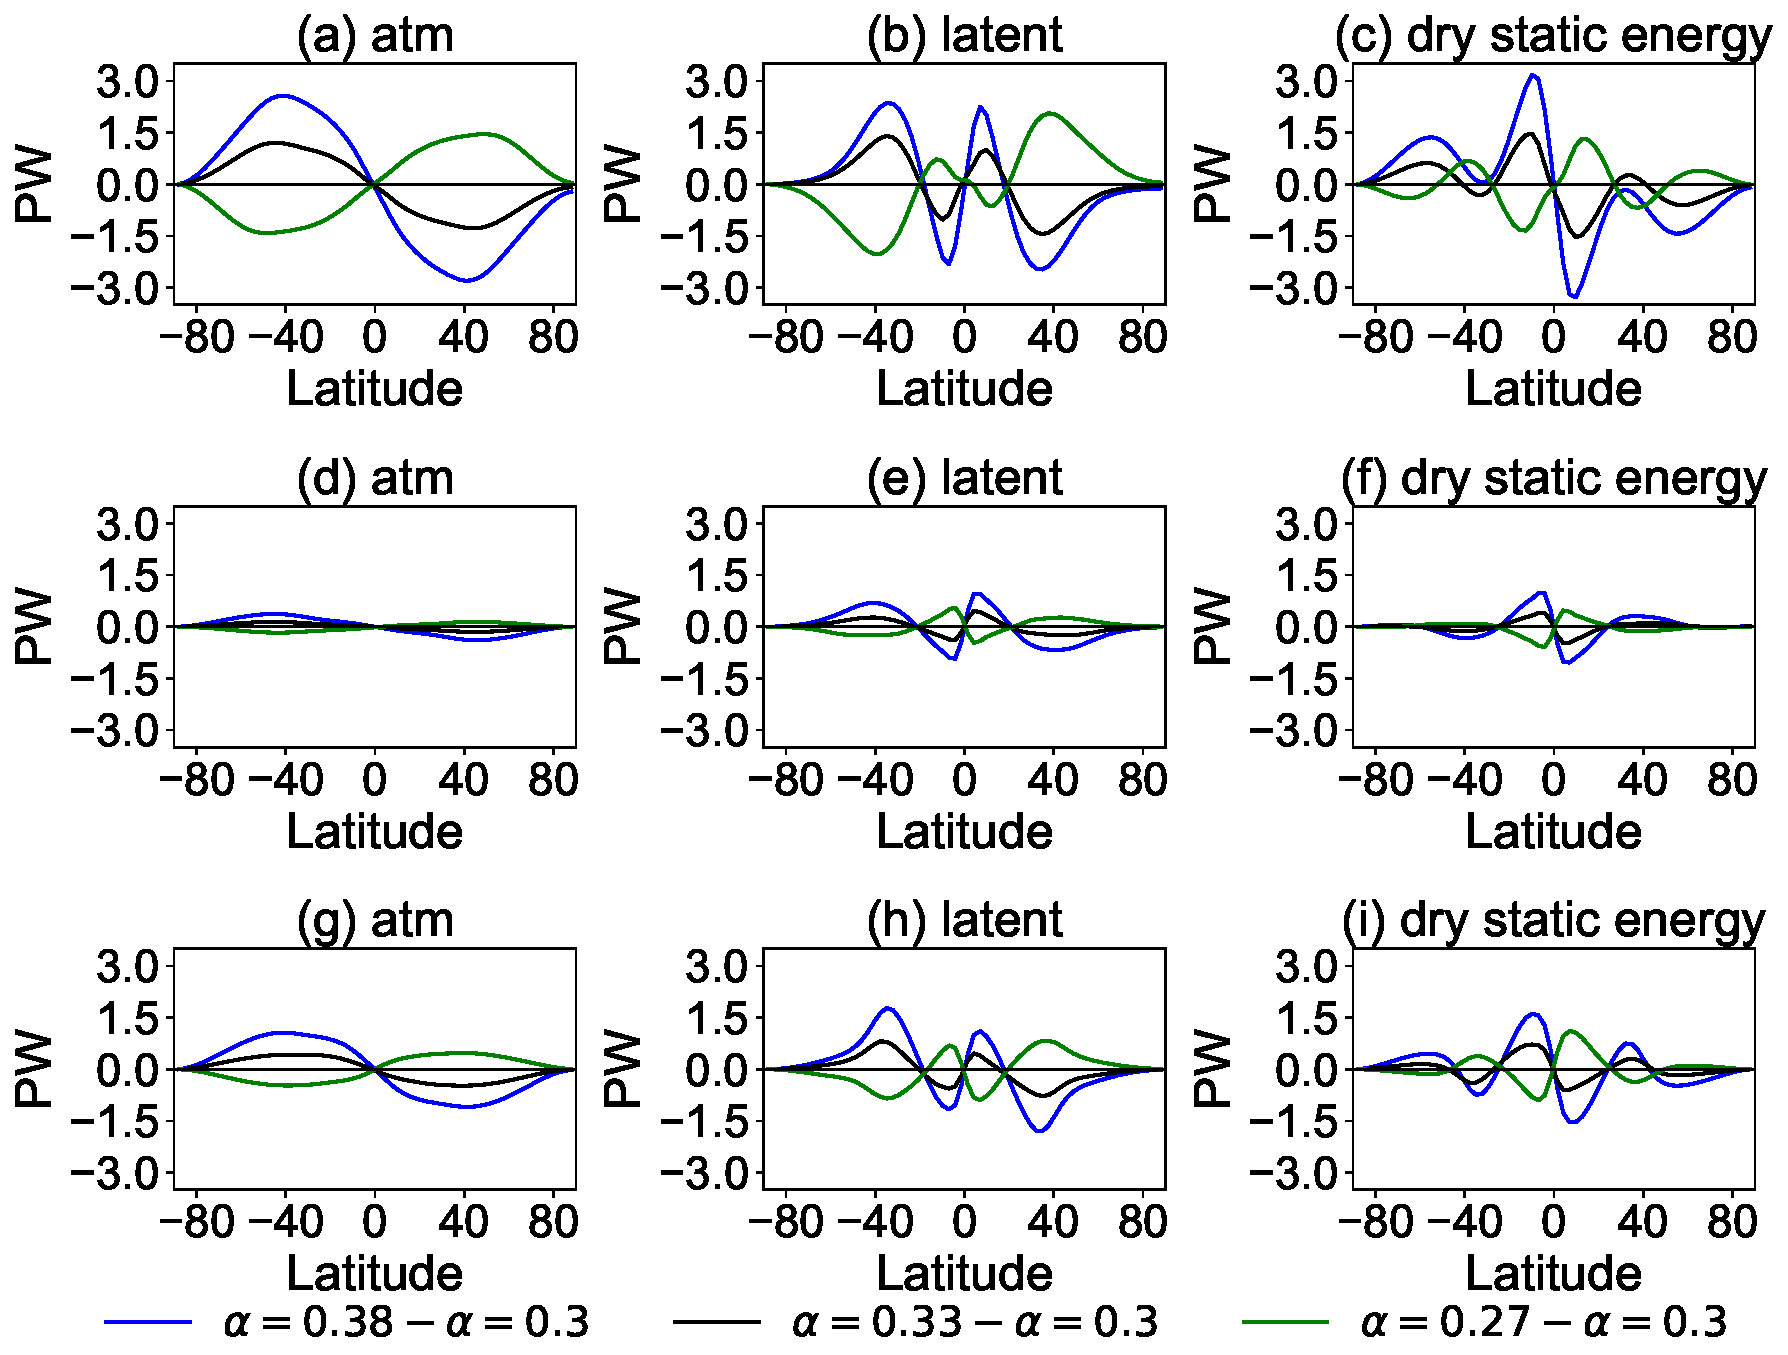
\includegraphics[width=0.9\linewidth]{{figs/polar_amp/heat_transport_bog_frierson_components_diff_test}.pdf}
	\caption[Changes in heat transport after varying the albedos]{As in \figref{fig:ht_transport}, but for the difference in heat transport between the experiments with different radiation schemes and various albedos. Blue, black and green solid lines indicates the difference between experiments where albedo is 0.38, 0.33 and 0.27 and the control experiment respectively.}
	\label{fig:ht_transport_diff}
\end{figure}

\begin{figure}[ht]
	\centering
	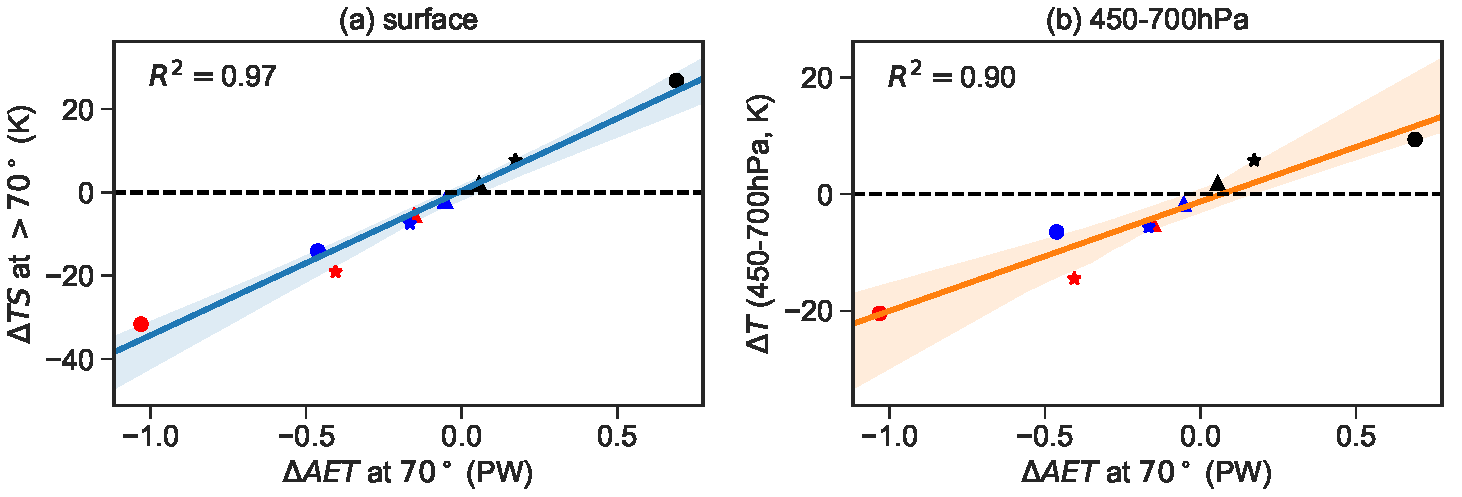
\includegraphics[width=0.8\linewidth]{figs/polar_amp/heat_transport_delta_ts.pdf}
	\caption[Changes of (a) surface temperature and (b) temperature at middle troposphere in polar region versus changes in atmospheric energy transport at $70^\circ$.]{(a) Changes of surface temperature poleward of $70^\circ$ versus changes in atmospheric energy transport (AET) at $70^\circ$ and the blue line is the linear regression of the two variables with the shading area indicating the 95\% confidence interval. The solid circles, stars and triangles denote the BOG, Frierson and RRTM schemes respectively, and red, blue and black markers represent the runs in which the albedos are changed from 0.3 to 0.38, 0.33 and 0.27 respectively. (b) Same as (a), but for temperature change in middle troposphere (450--700 hPa).}
	\label{fig:delta_ht_ts}
\end{figure}


%\begin{figure}[ht]
%	\centering
%	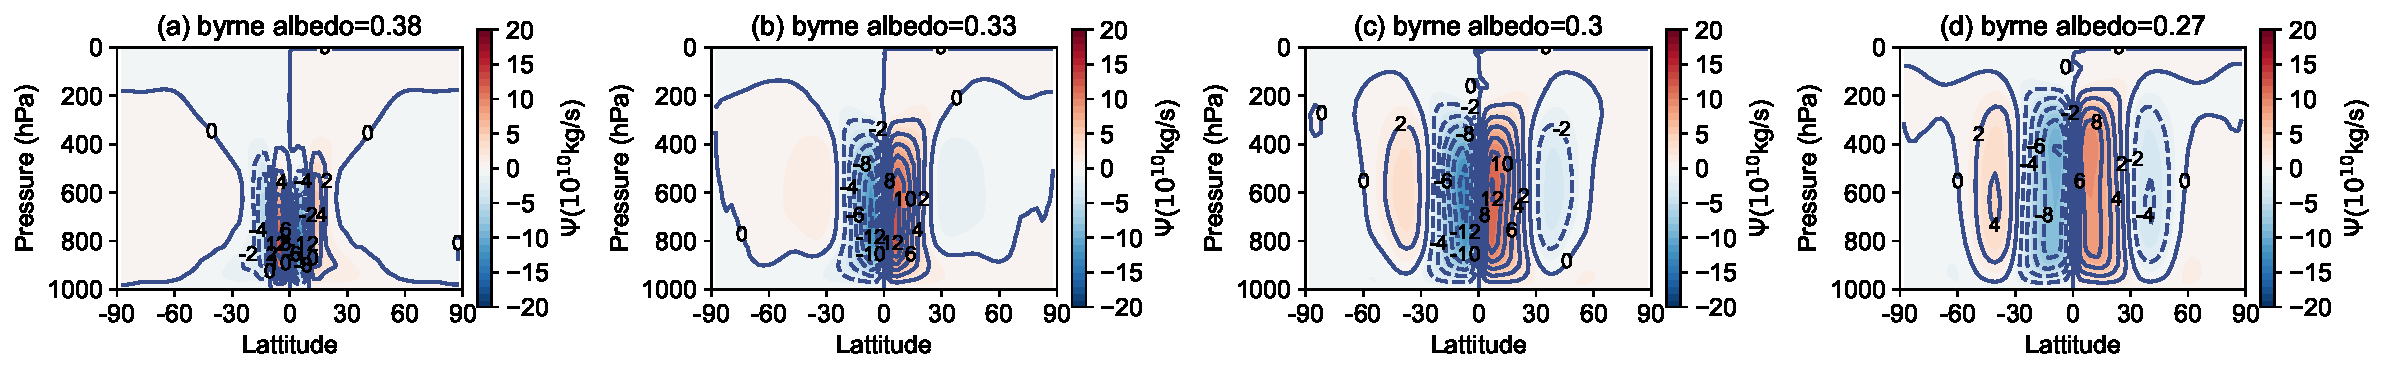
\includegraphics[width=1.0\linewidth]{{figs/polar_amp/fig_three_rad_scheme_coolwarm_4_albedos/hadley_cell_byrne}.pdf}
%	\caption{Zonally averaged meridional
%		overturning circulation of the
%		atmosphere ($kg\cdot  s^{-1}$) in BOG radiation scheme with four different albedos, where streamfunction $\Psi$ is shown in contour.}
%	\label{fig:haleycell_bog}
%\end{figure}

%One remaining question about BOG radiation scheme is the strange behaviour when the albedo is 0.38, e.g. the concave in the difference of zonal mean surface temperature near the equator, and the reversal of latent heat transport near equator illustrated in red line in \figref{fig:ht_transport}d. Given the fact of the reversal of latent heat transport, it is helpful to check the Hadley cell circulation in low latitudes. As depicted in \figref{fig:haleycell_bog}, the Hadley circulation is reversed when albedo is 0.38 in BOG radiation scheme, and the overturning circulation is weak compared to other experiments where albedo is 0.27, 0.3 and 0.33, implying that the meridional velocity may be reversed in the experiment (\figref{fig:v_zonal}a). Therefore, the reversal of meridional velocity in the tropical region explains the opposite direction of latent heat transport ($H_{LH} = \int_0^{2\pi} \int_{\text{bottom}}^{\text{top}} \rho v L_vq\text{d}z ~ a \cos\phi ~ \text{d}\lambda$). As for the concave in the difference of zonal mean  surface temprature, the reversal of the latent heat transport also provide some insights, that is the latent energy is transported off the equator when albedo is 0.38, while it is transported equatorward in other experiments from BOG radiation scheme.  In addition, the difference of latent heat transport between albedo is 0.38 and the control run is extremely larger than others (\figref{fig:ht_transport_diff}d) also proves that point.

%\begin{figure}[ht]
%	\centering
%	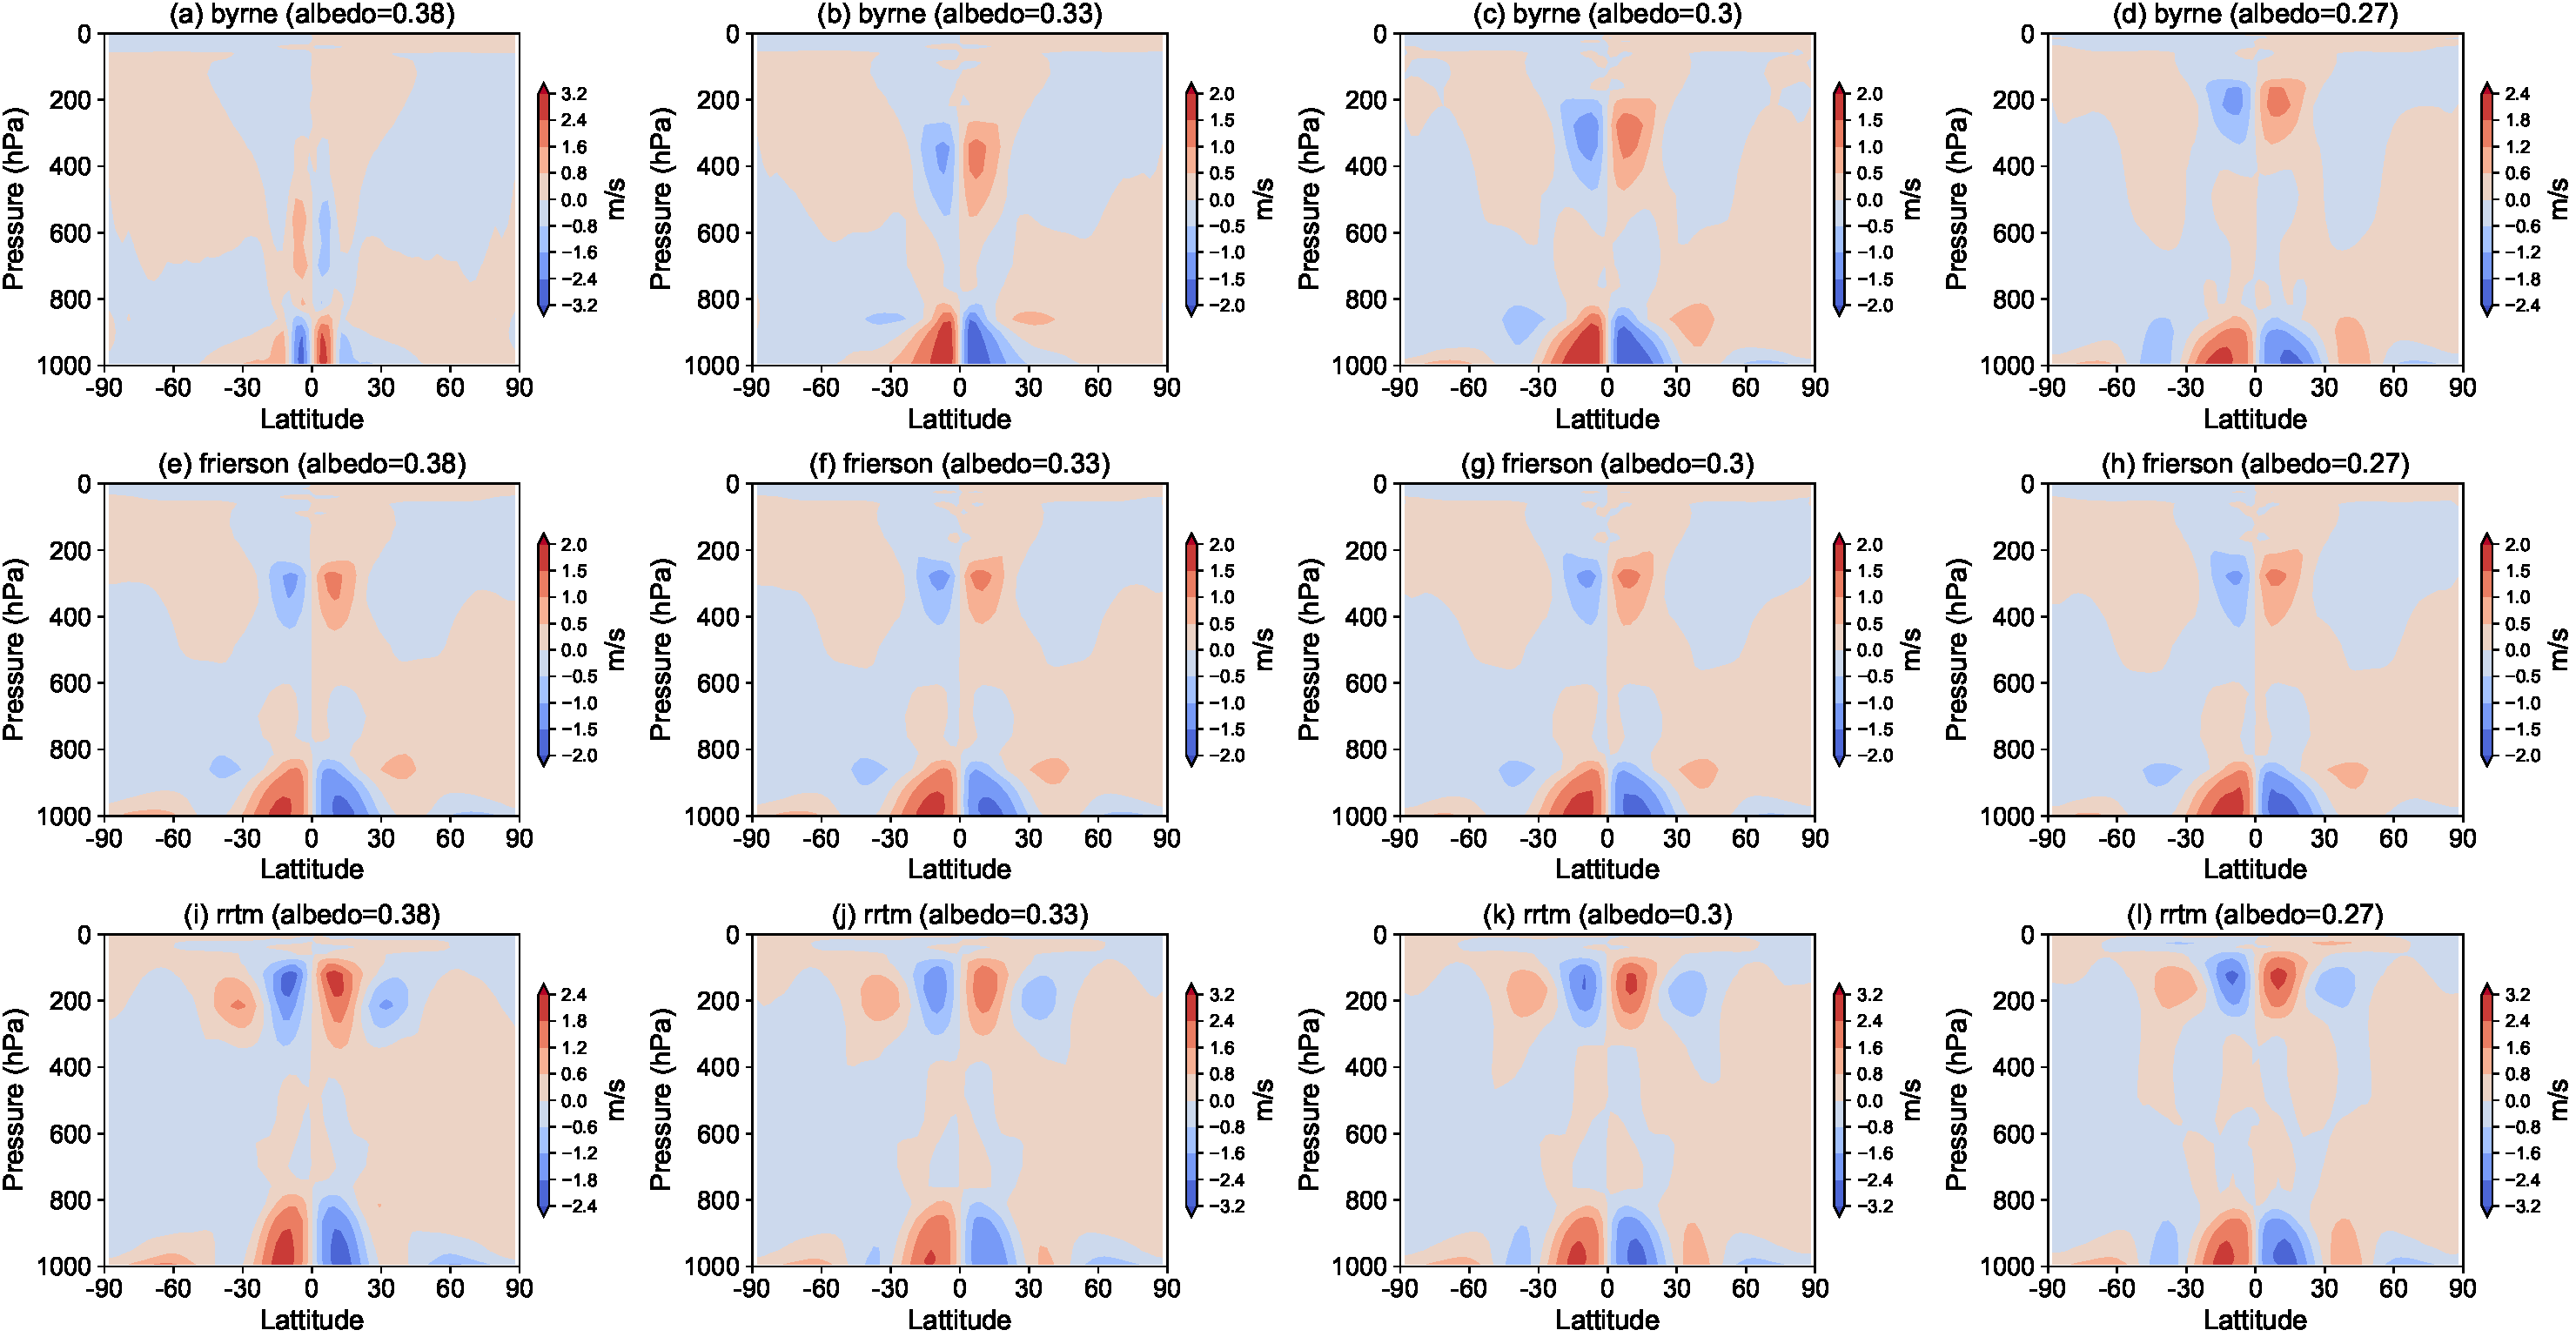
\includegraphics[width=1.0\linewidth]{{figs/polar_amp/fig_three_rad_scheme_coolwarm_4_albedos/vcomp_vert_profile_all_three_albedos}.pdf}
%	\caption{Annual mean and zonally averaged meridional velocity vertical profiles for the experiments with different radiation schemes and albedos.}
%	\label{fig:v_zonal}
%\end{figure}

%In summary, the change of latent heat transport with different albedos may be related to the zonal mean surface temperature change so as to the polar amplification. What's more, the reversal of meridional velocity and the ensuing reversals of Hadley cell circulation and latent heat transport give an explanation for the abnormal behaviours of the experiment with albedo is 0.38 in BOG radiation scheme.


%\subsection{Effect of climate feedbacks}
\subsection{Decomposition of surface temperature response}
\label{sec:climate_feedbacks_temp_decomp}

%\subsubsection{Decomposition of surface temperature response}

In \secref{sec:method_radiative_kernel}, with the aid of radiative kernel method, we have obtained the zonal mean radiative feedback parameters for BOG, Frierson and RRTM radiation schemes in Isca model (\figref{fig:all_feedbacks}), which enables us to investigate the relative importance of each feedback to zonal mean surface temperature change. Following \cite{Feldl2013} and \cite{Kim2018}, we decompose the surface temperature change into various components after rearranging the \Eqref{eq:delta_R_relation}:

% we have decomposed the climate feedbacks into Planck feedback, lapse rate feedback, water vapor feedback but without cloud feedback, which is different from 

\begin{equation}
	\Delta T_s = \frac{1}{\overline{\lambda_P}}\left[\Delta R -\left(\lambda'_P+\sum_{i}\lambda_{NP_i}\right)\Delta T_s-\Delta F\right],
	\label{eq:decomp_Ts}
\end{equation}
where $\overline{\lambda_P}$ designates the global mean Planck feedback, by which all the feedbacks will be normalized, including the local deviation of Planck feedback ($\lambda'_P$) from its global mean and all the other non-Planck feedbacks ($\lambda_{NP_i}$). As mentioned earlier, the cloud feedback and albedo feedback are not included in the experiments and thus lapse rate and water vapor feedback are the only two non-Planck feedbacks in \Eqref{eq:decomp_Ts}. $\Delta R$ is the net TOA radiative flux and it should be equal to the change in the convergence of horizontal atmospheric heat flux, referred as the heat transport term. $\Delta F$ is the forcing after changing albedos estimated by fixed-SST method.


The contributions to the zonal mean surface temperature change in BOG, Frierson and RRTM radiation schemes are displayed in \figref{fig:delta_ts_decomp}. We first look at the results from RRTM radiation scheme as it provides a more realistic radiation scheme. As shown in \figsref{fig:delta_ts_decomp}g-i, the sum of different components (red thick dash-dotted line) reproduces the actual surface temperature change (blue thick solid line) in RRTM scheme either in cooling (\figsref{fig:delta_ts_decomp}g, h) or warming (\figref{fig:delta_ts_decomp}i) cases, which implies we can analyze the relative importance of various components. As analyzed by \cite{Pithan2014}, the Planck feedback itself will automatically cause greater temperature change in high latitudes. In fact, according to Stefan-Boltzmann law, the longwave radiation emitted by earth surface ($R_s$) is
\begin{equation}
	R_s = \epsilon\sigma T^4,
\end{equation}
where $\epsilon$ is surface emissivity, which is close to 1, and $\sigma$ the Stefan-Boltzmann constant with value of $5.67\times 10^{-8}$ Wm$^{-2}$K$^{-1}$. Assuming there is a uniform radiation disturbance ($\Delta R$) at TOA, the surface temperature has to change by $\Delta T$ to balance $\Delta R$, and $\Delta T$ given by

\begin{equation}
\Delta T =\frac{\Delta R_s}{4\epsilon\sigma T^3}=\frac{\Delta R}{4\epsilon\sigma T^3},
\end{equation}
in which $\Delta R_s$ is the radiation change at the surface. It is clear that the temperature response ($\Delta T$) is large when the temperature ($T$) is low (e.g. polar region) and $\Delta T$ is small when T is relative high (e.g. tropical region). Therefore, the temperature response from Planck feedbacks (orange lines in \figsref{fig:delta_ts_decomp}g-i) is large at high latitudes and small at low latitudes. It should be pointed out that the Planck feedback is a negative feedback, but here the \figref{fig:delta_ts_decomp} shows the local deviation of Planck feedback from its global mean value and that is why the temperature response is negative in \figsref{fig:delta_ts_decomp}g, h, and positive in \figref{fig:delta_ts_decomp}i. For the temperature response caused by lapse rate feedback (green solid lines in \figsref{fig:delta_ts_decomp}g-i), it is positive in polar region and negative in tropical region in warming case and the signs are opposite in cooling case, indicating that the lapse rate feedback will amplify the temperature response in high latitudes. The positive lapse rate feedback in polar region is due to the bottom-heavy warming/cooling vertical structure (\figref{fig:vert_temp_diff}). Our finding in the warming case is consistent with result under equinox insolation in \cite{Kim2018}, but they show that things are different under seasonal and annual mean insolation conditions in which the lapse rate feedback is globally negative \citep[see Fig. S1 of][]{Kim2018}. This is because the induced temperature change is not enough to form an inversion layer near the surface \citep{Kim2018}. %\figref{fig:kim2018_lapserate}

% different from the results of \cite{Kim2018}, where the lapse rate feedback is globally negative under seasonal insolation.

%The stable atmospheric structure in polar region making the lapse rate feedback positive

\begin{figure}[ht]
	\centering
	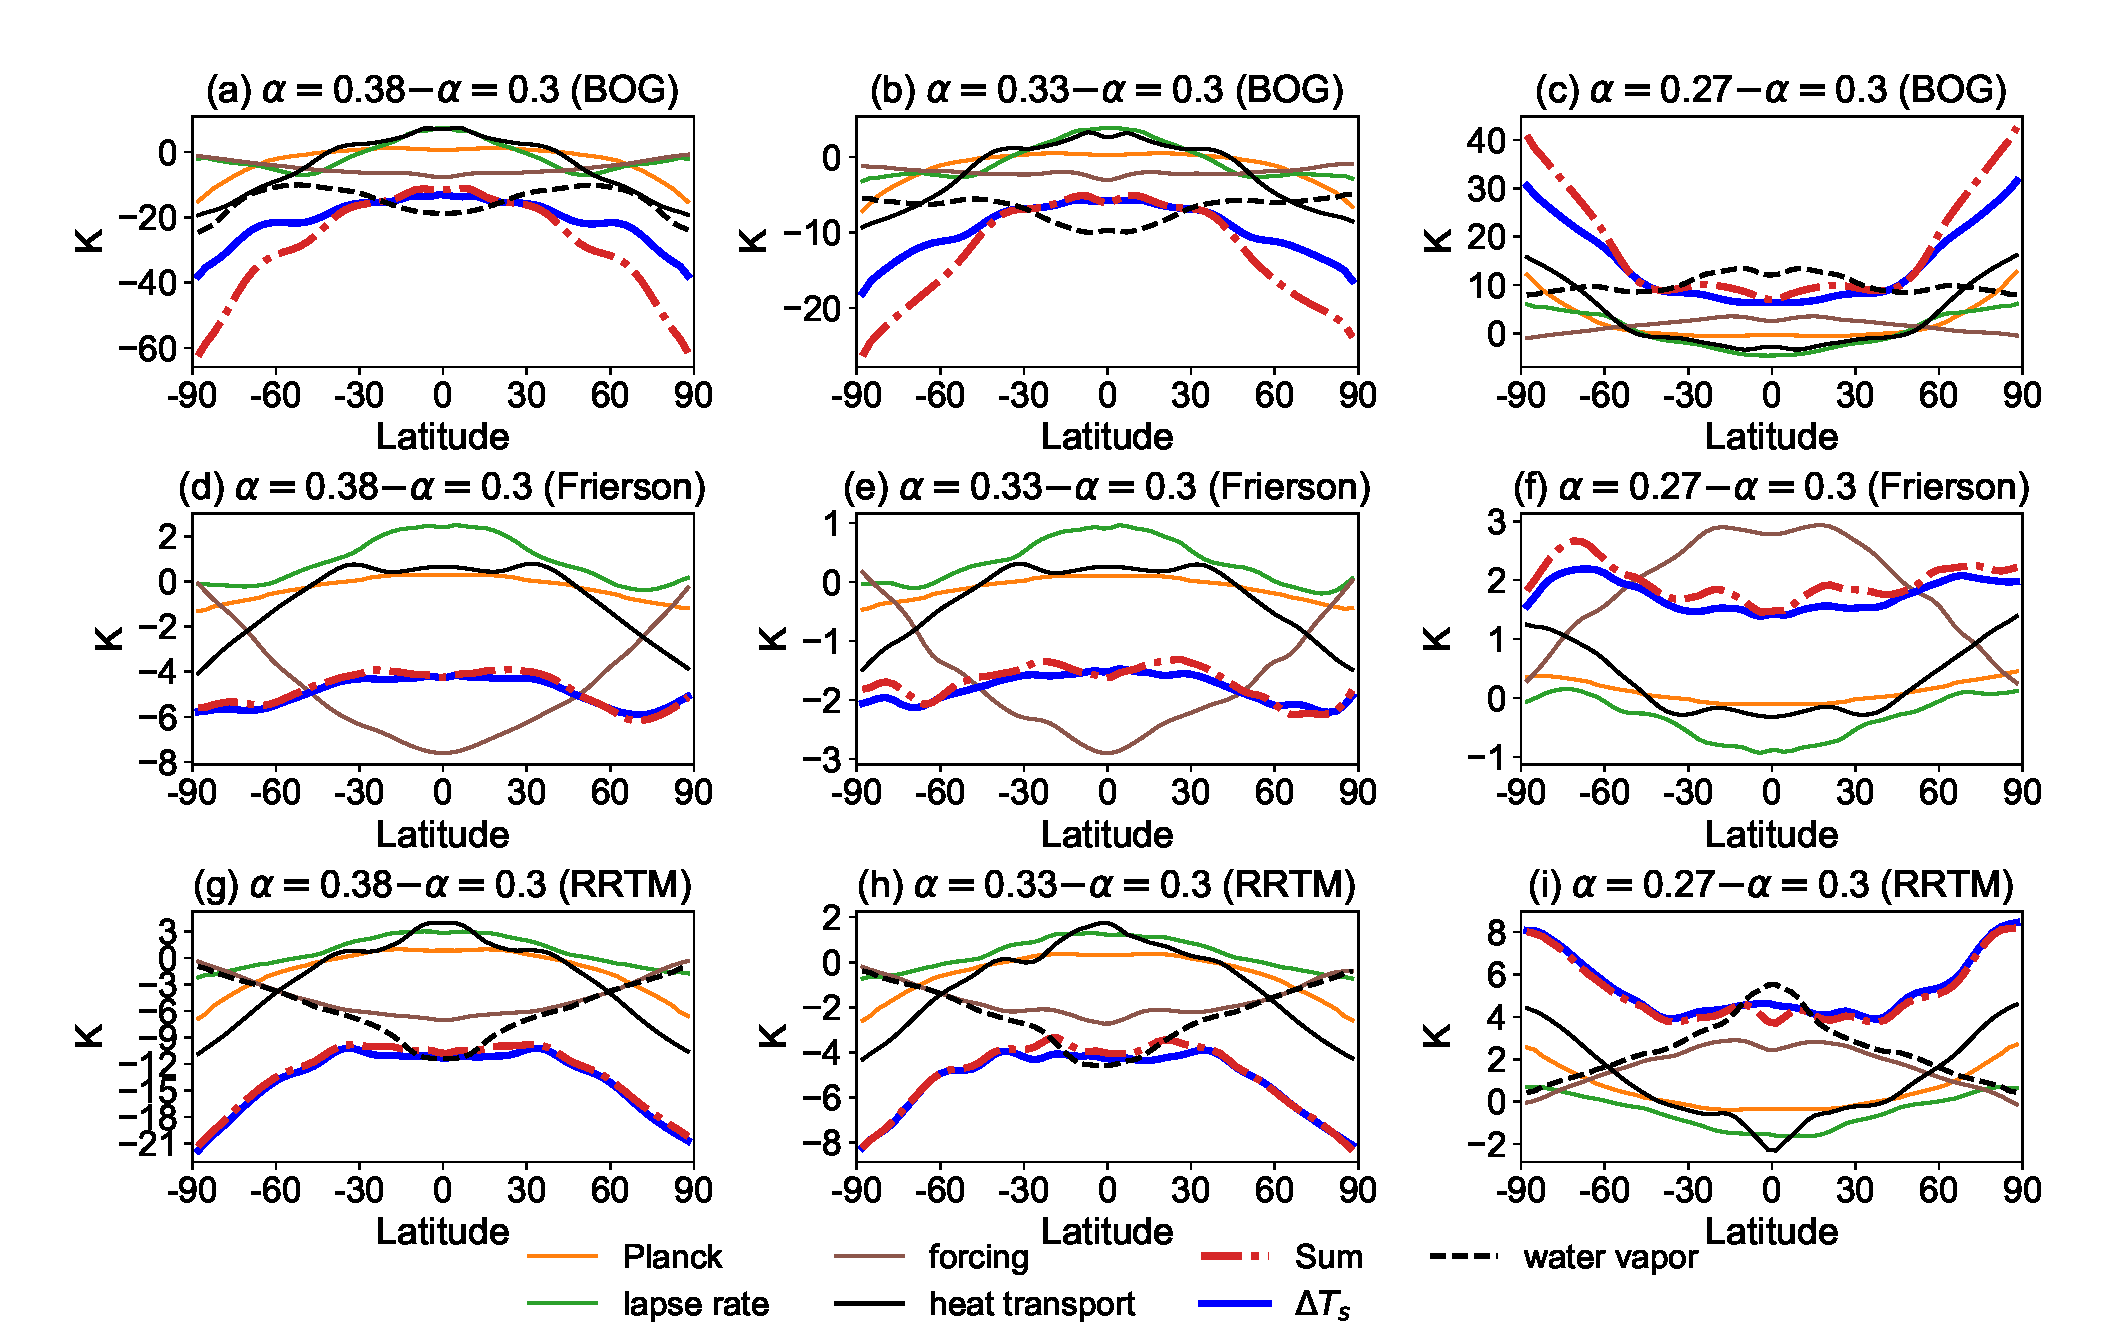
\includegraphics[width=1.0\linewidth]{figs/polar_amp/delta_ts_decomp}
	%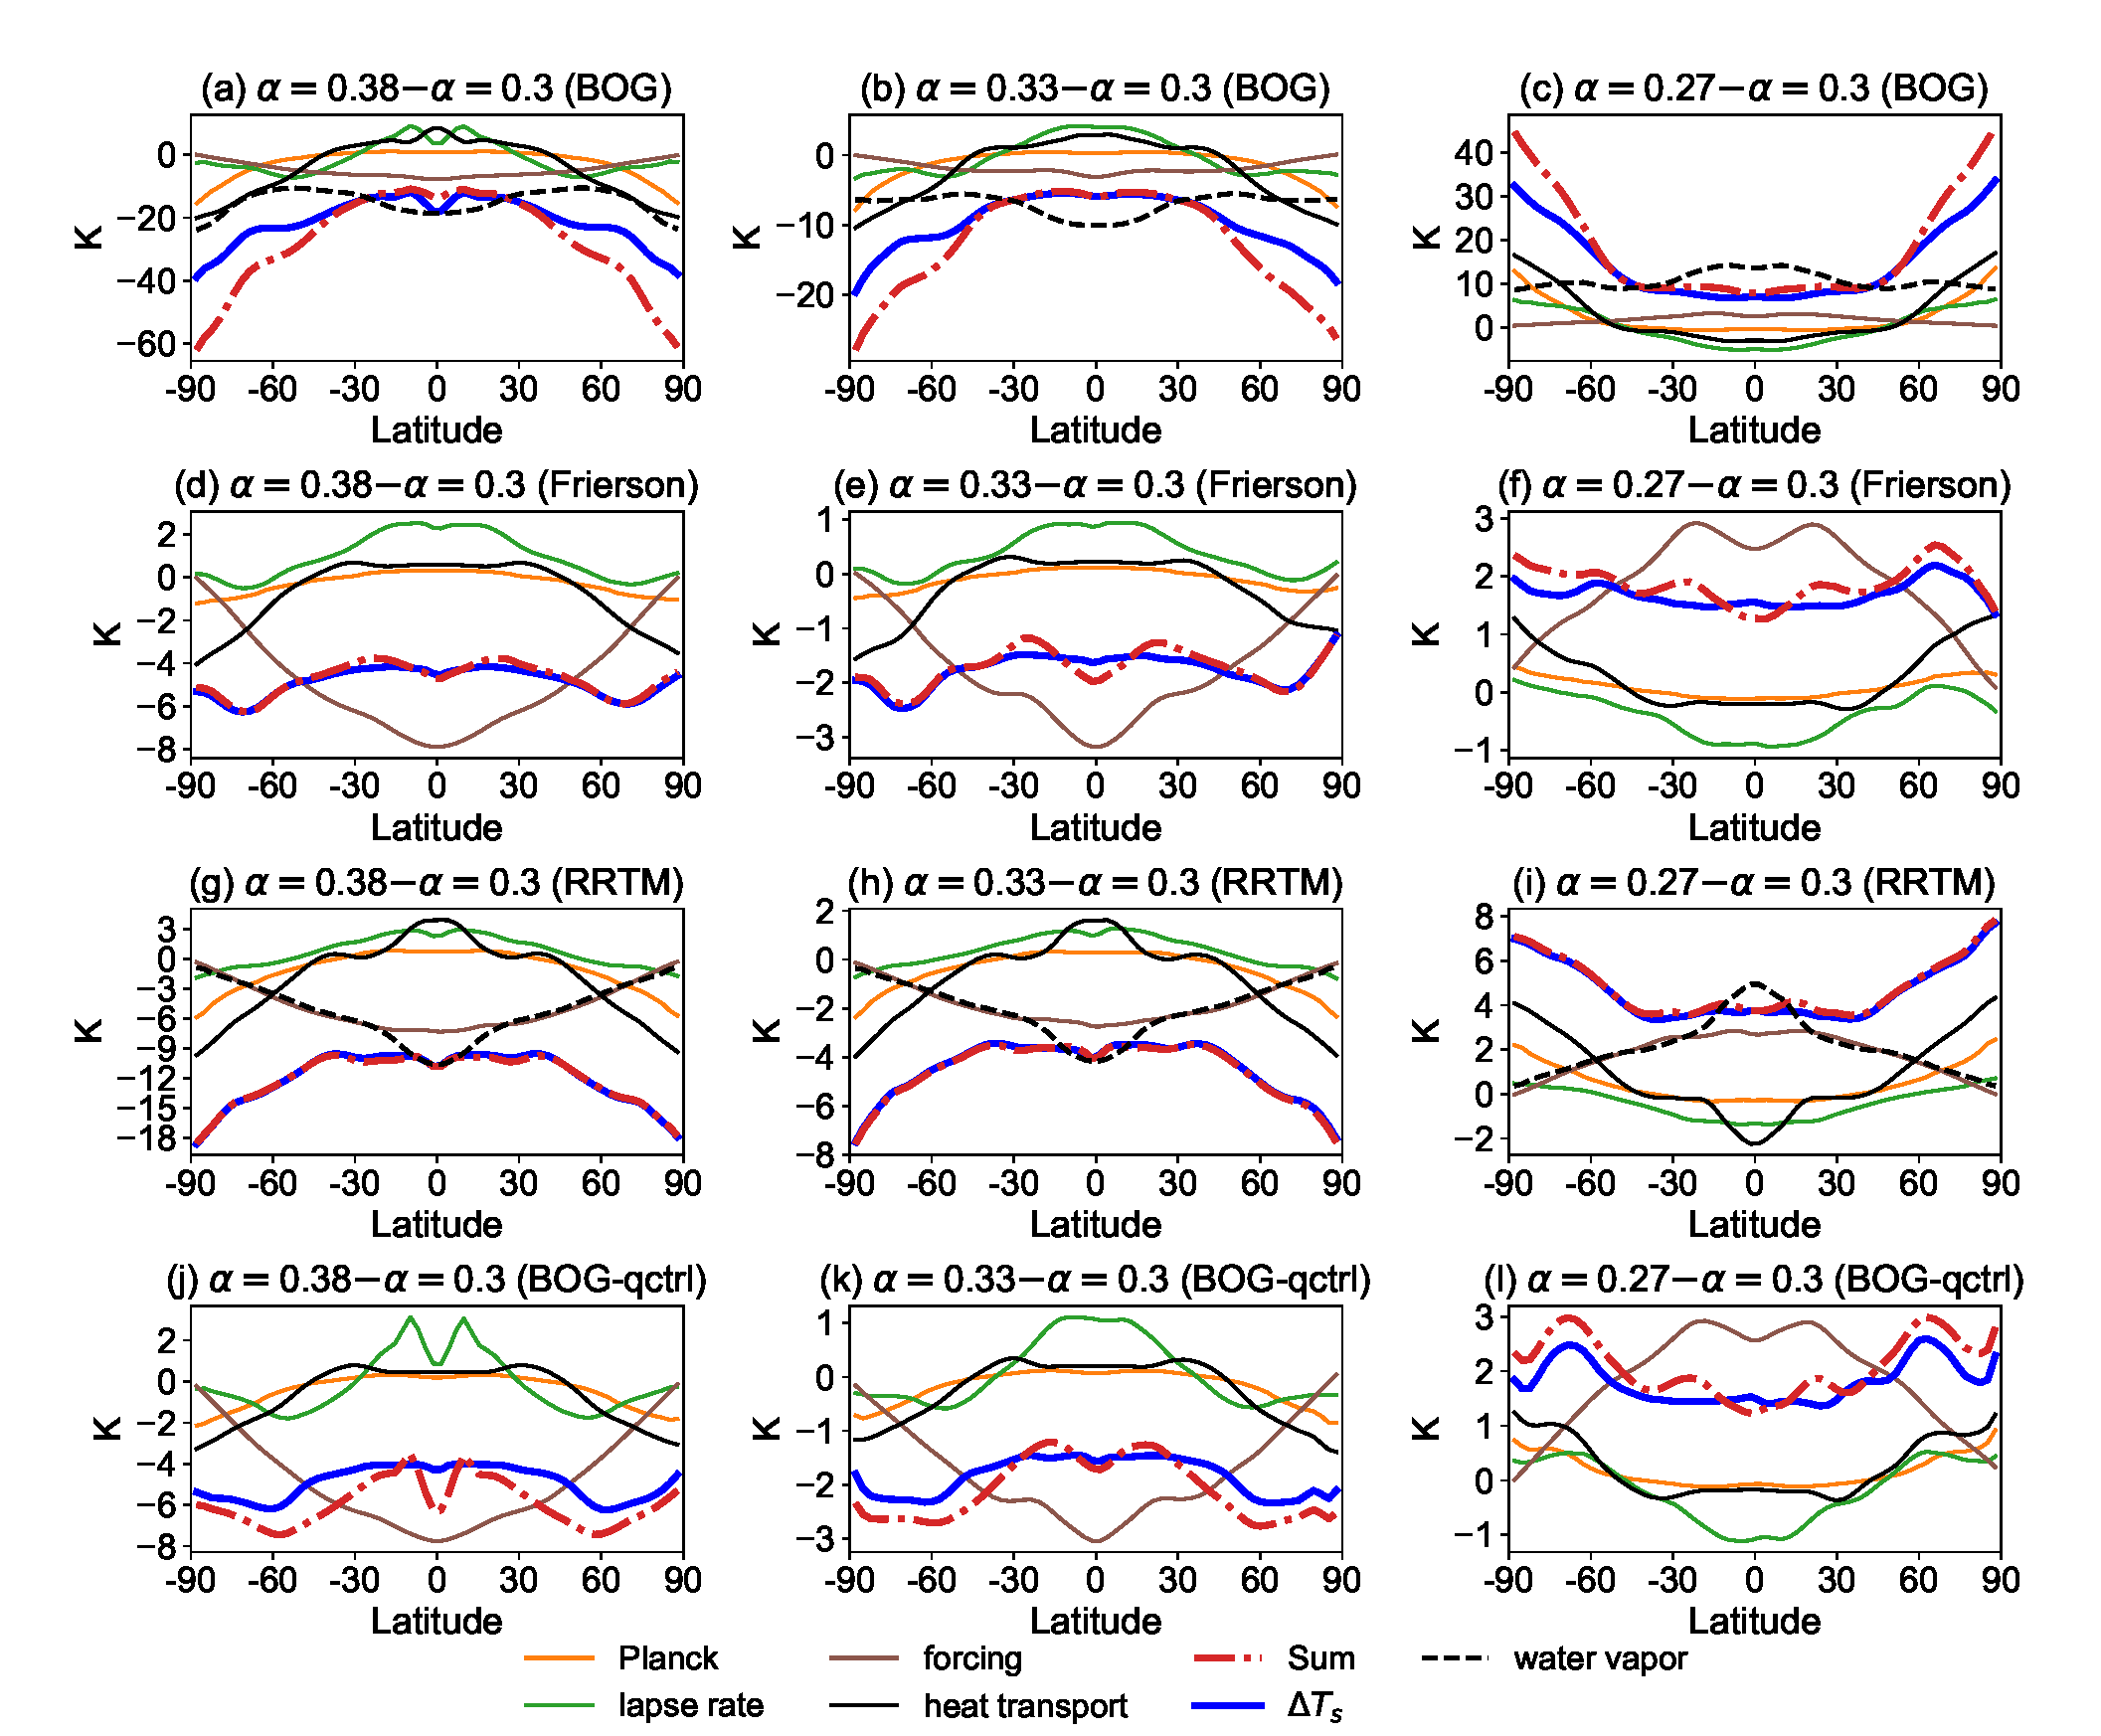
\includegraphics[width=1.0\linewidth]{figs/polar_amp/delta_ts_decomp_q.pdf}
	\caption[Zonal and annual mean contributions of surface temperature changes from forcing, heat transport and climate feedbacks]{Zonal and annual mean contributions of surface temperature changes for (a)-(c) BOG scheme, (d)-(f) Frierson scheme, (g)-(i) RRTM schemes and (j)-(l) BOG scheme without moisture feedback respectively. The components include Planck feedback (orange), lapse rate feedback (green), forcing (brown), water vapor feedback (black dashed) and heat transport (black solid), all of which are weighted by global and annual mean of Planck feedback following \cite{Feldl2013a} and \cite{Kim2018}. The sum of the different components is shown in thick red dash-dotted lines and the surface temperature change in experiments is indicated by thick blue lines. The first, second and third columns are for experiments when albedo is changed from 0.3 to 0.38, 0.33 and 0.27 respectively.}
	\label{fig:delta_ts_decomp} 
\end{figure}

% \begin{figure}[ht] %
% 	\centering
% 	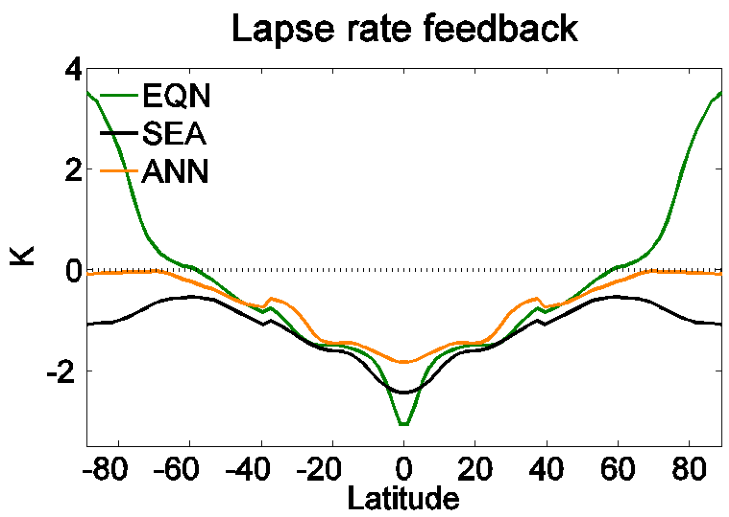
\includegraphics[width=.6\linewidth]{figs/polar_amp/Kim2018_lapserate}
% 	\caption{Zonal- and time-mean partial temperature changes (K) attributed to lapse rate feedback in GFDL AM2 under equinox (EQN, green), seasonal (SEA, black), and annual mean (ANN, orange) insolation. Adapted from Figure S1 of \cite{Kim2018}.}
% 	\label{fig:kim2018_lapserate}
% \end{figure}

The heat transport contributes most to the surface temperature change in polar region both in cooling and warming case in our study, but it is different from the calculation of \cite{Pithan2014}, where they find that the temperature related feedbacks contribute most to the Arctic warming when there is a surface albedo feedback. When there is a lack of surface albedo feedback, the heat transport is also the largest contributor to the polar amplification under seasonal solar radiation according to \cite{Kim2018}. In the warming case (\figref{fig:delta_ts_decomp}i), the heat transport cools the low latitudes and warms the high latitudes, which decreases the large meridional temperature and energy imbalance gradients. As illustrated in \figsref{fig:delta_ts_decomp}g-i, the water vapor feedbacks contribute more to the tropical warming or cooling rather than to polar regions, which is consistent with the conclusion of \cite{Pithan2014}. But water vapor does have effect on the temperature change due to the enlarged climate sensitivity \citep{Langen2012}. In fact, the temperature responses due to water vapor feedbacks in BOG scheme (black dashed lines in \figsref{fig:delta_ts_decomp}a-c) are different from that in RRTM schemes. They do not tend to zero as latitude increases. Instead, they are relative flat at high latitudes, which could possibly be used to explain the abnormal surface temperature response in BOG scheme. Regarding the forcing (brown lines in \figsref{fig:delta_ts_decomp}g-i) due to the change of albedos, it is larger in low latitudes than in high latitudes as the solar radiation is strong at low latitudes, and hence it will amplify the temperature change at low latitudes.

 \begin{figure}[ht]
    \centering
	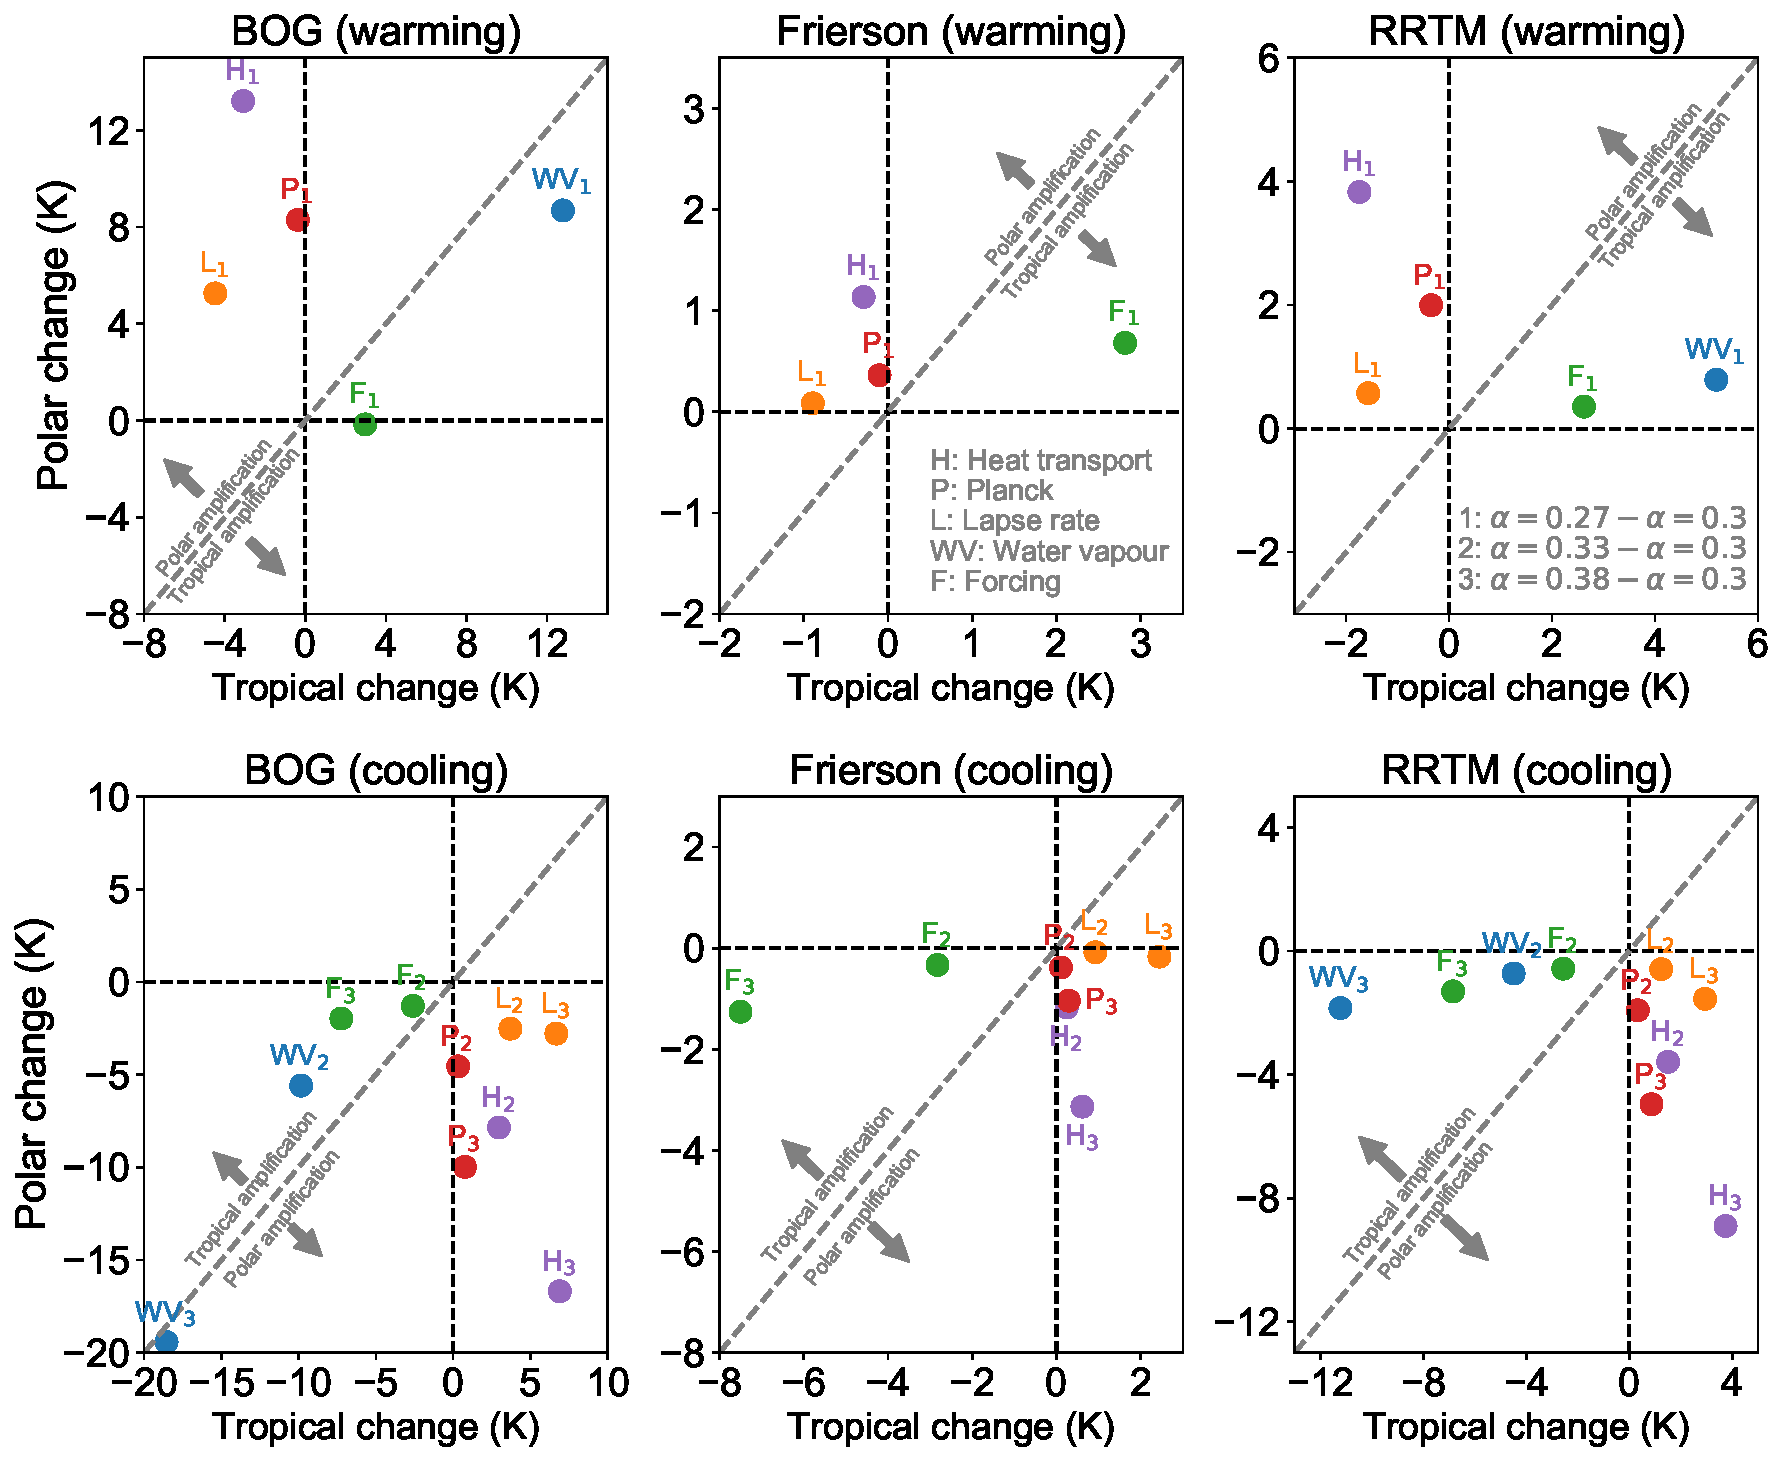
\includegraphics[width=0.9\textwidth]{figs/polar_amp/contributions_to_polar_amplification.pdf}
	\caption[The contributions of various factors to polar versus tropical temperature changes from a TOA perspective]{The contributions of various factors to polar versus tropical temperature changes from a TOA perspective. The factors are shown in the legend, and those above the 1:1 line contribute to polar amplification, whereas feedbacks below the line oppose polar amplification. The upper and bottom panels are for the warming (subscript 1) and cooling (subscripts 2 and 3) cases respectively. The titles of each figure indicate the radiation schemes used in the runs.}
	\label{fig:contribution_pole_vs_tropic}
\end{figure}

The roles of lapse rate feedback, Planck feedback and heat transport in BOG (\figsref{fig:delta_ts_decomp}a-c) and Frierson (\figsref{fig:delta_ts_decomp}d-f) schemes are similar to those in RRTM scheme, except the role of water vapor feedback in BOG scheme, which is much larger at high latitudes compared to others. One strange thing is the sum of these contributions is greater than the actual temperature response at high latitude in BOG scheme, for which a possible reason is that the decomposition of the surface temperature change is linear and some non-linear factors may have an influence at the high latitudes. We can see that after the water vapor feedback being disabled in BOG scheme, the sum of these various components is close to $\Delta T_s$ (\figsref{fig:delta_ts_decomp}j-l), indicating that the non-linear effect is possible associated with water vapor. 

%\begin{figure}[ht] %[ht]
%	\centering
%	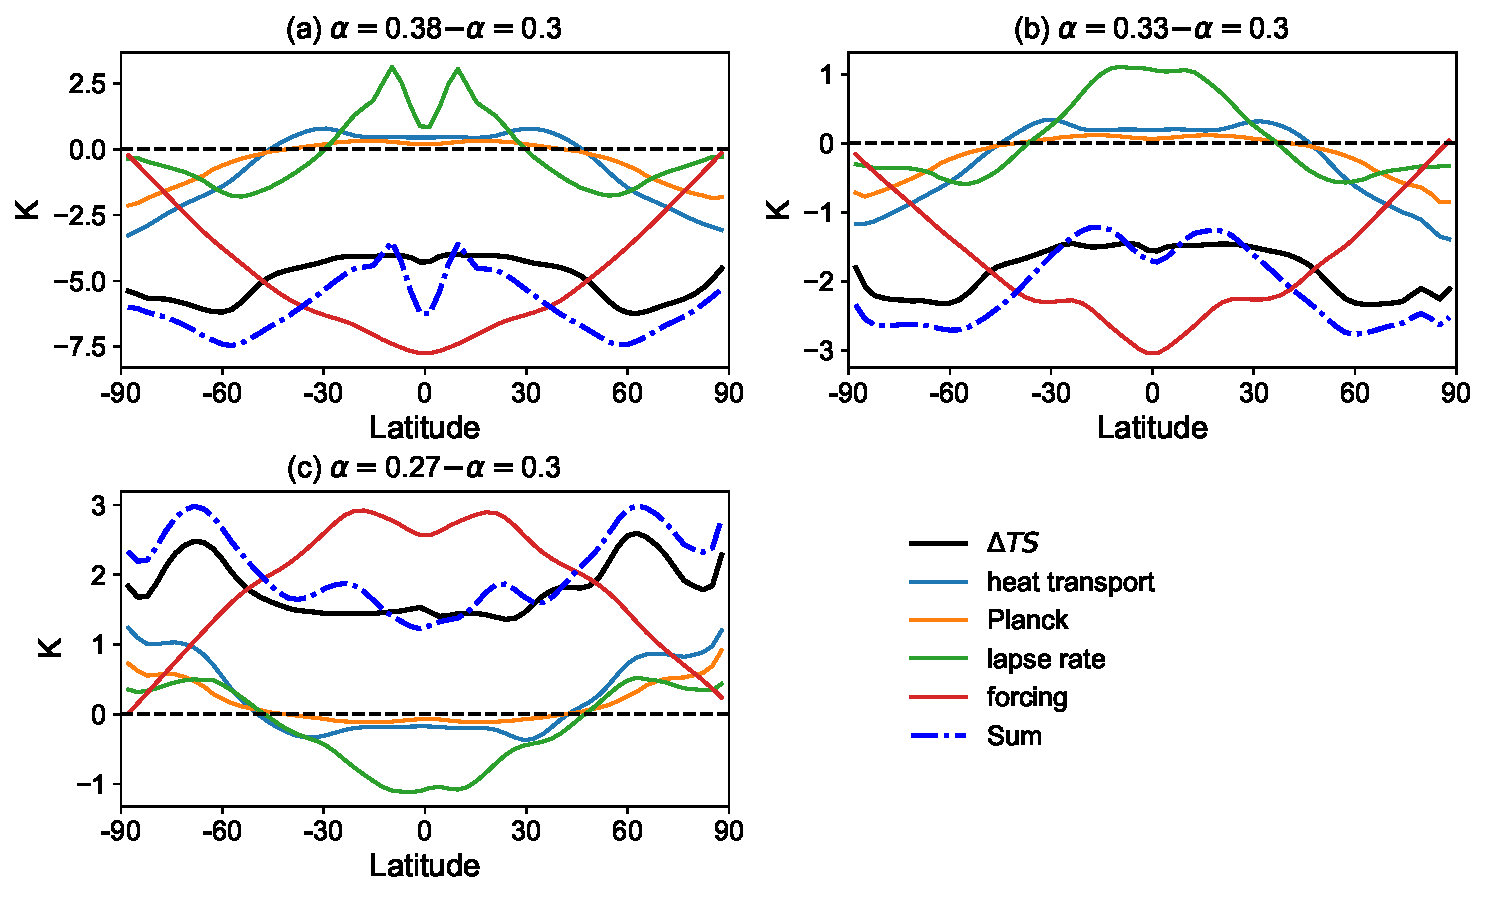
\includegraphics[width=0.8\linewidth]{figs/polar_amp/ts_decomp/delta_ts_decomp_fixed_q_byrne}
%	\caption{Zonal and annual mean contributions of surface temperature changes for (a)-(c) BOG radiation scheme without moisture feedbacks.}
%	\label{fig:delta_ts_decomp_bog_no_q_fb}
%\end{figure}

\section{Discussion and summary}
\label{sec:polar_amplification_summary}

In this chapter, we employ the Isca model to study the zonal mean surface temperature change in aquaplanet simulation with various radiation schemes and albedos in order to quantify the different mechanisms that could lead to polar amplification of surface temperature change under equinox insolation. Two gray radiation schemes, BOG and Frierson, and one full radiation scheme, RRTM, are used in the simulations. The BOG scheme shows the largest surface temperature change and polar amplification, while Frierson scheme shows the weakest surface temperature change when changing albedos. %, which is a way to disturb the radiation balance at TOA.

\begin{figure}[ht]
    \centering
	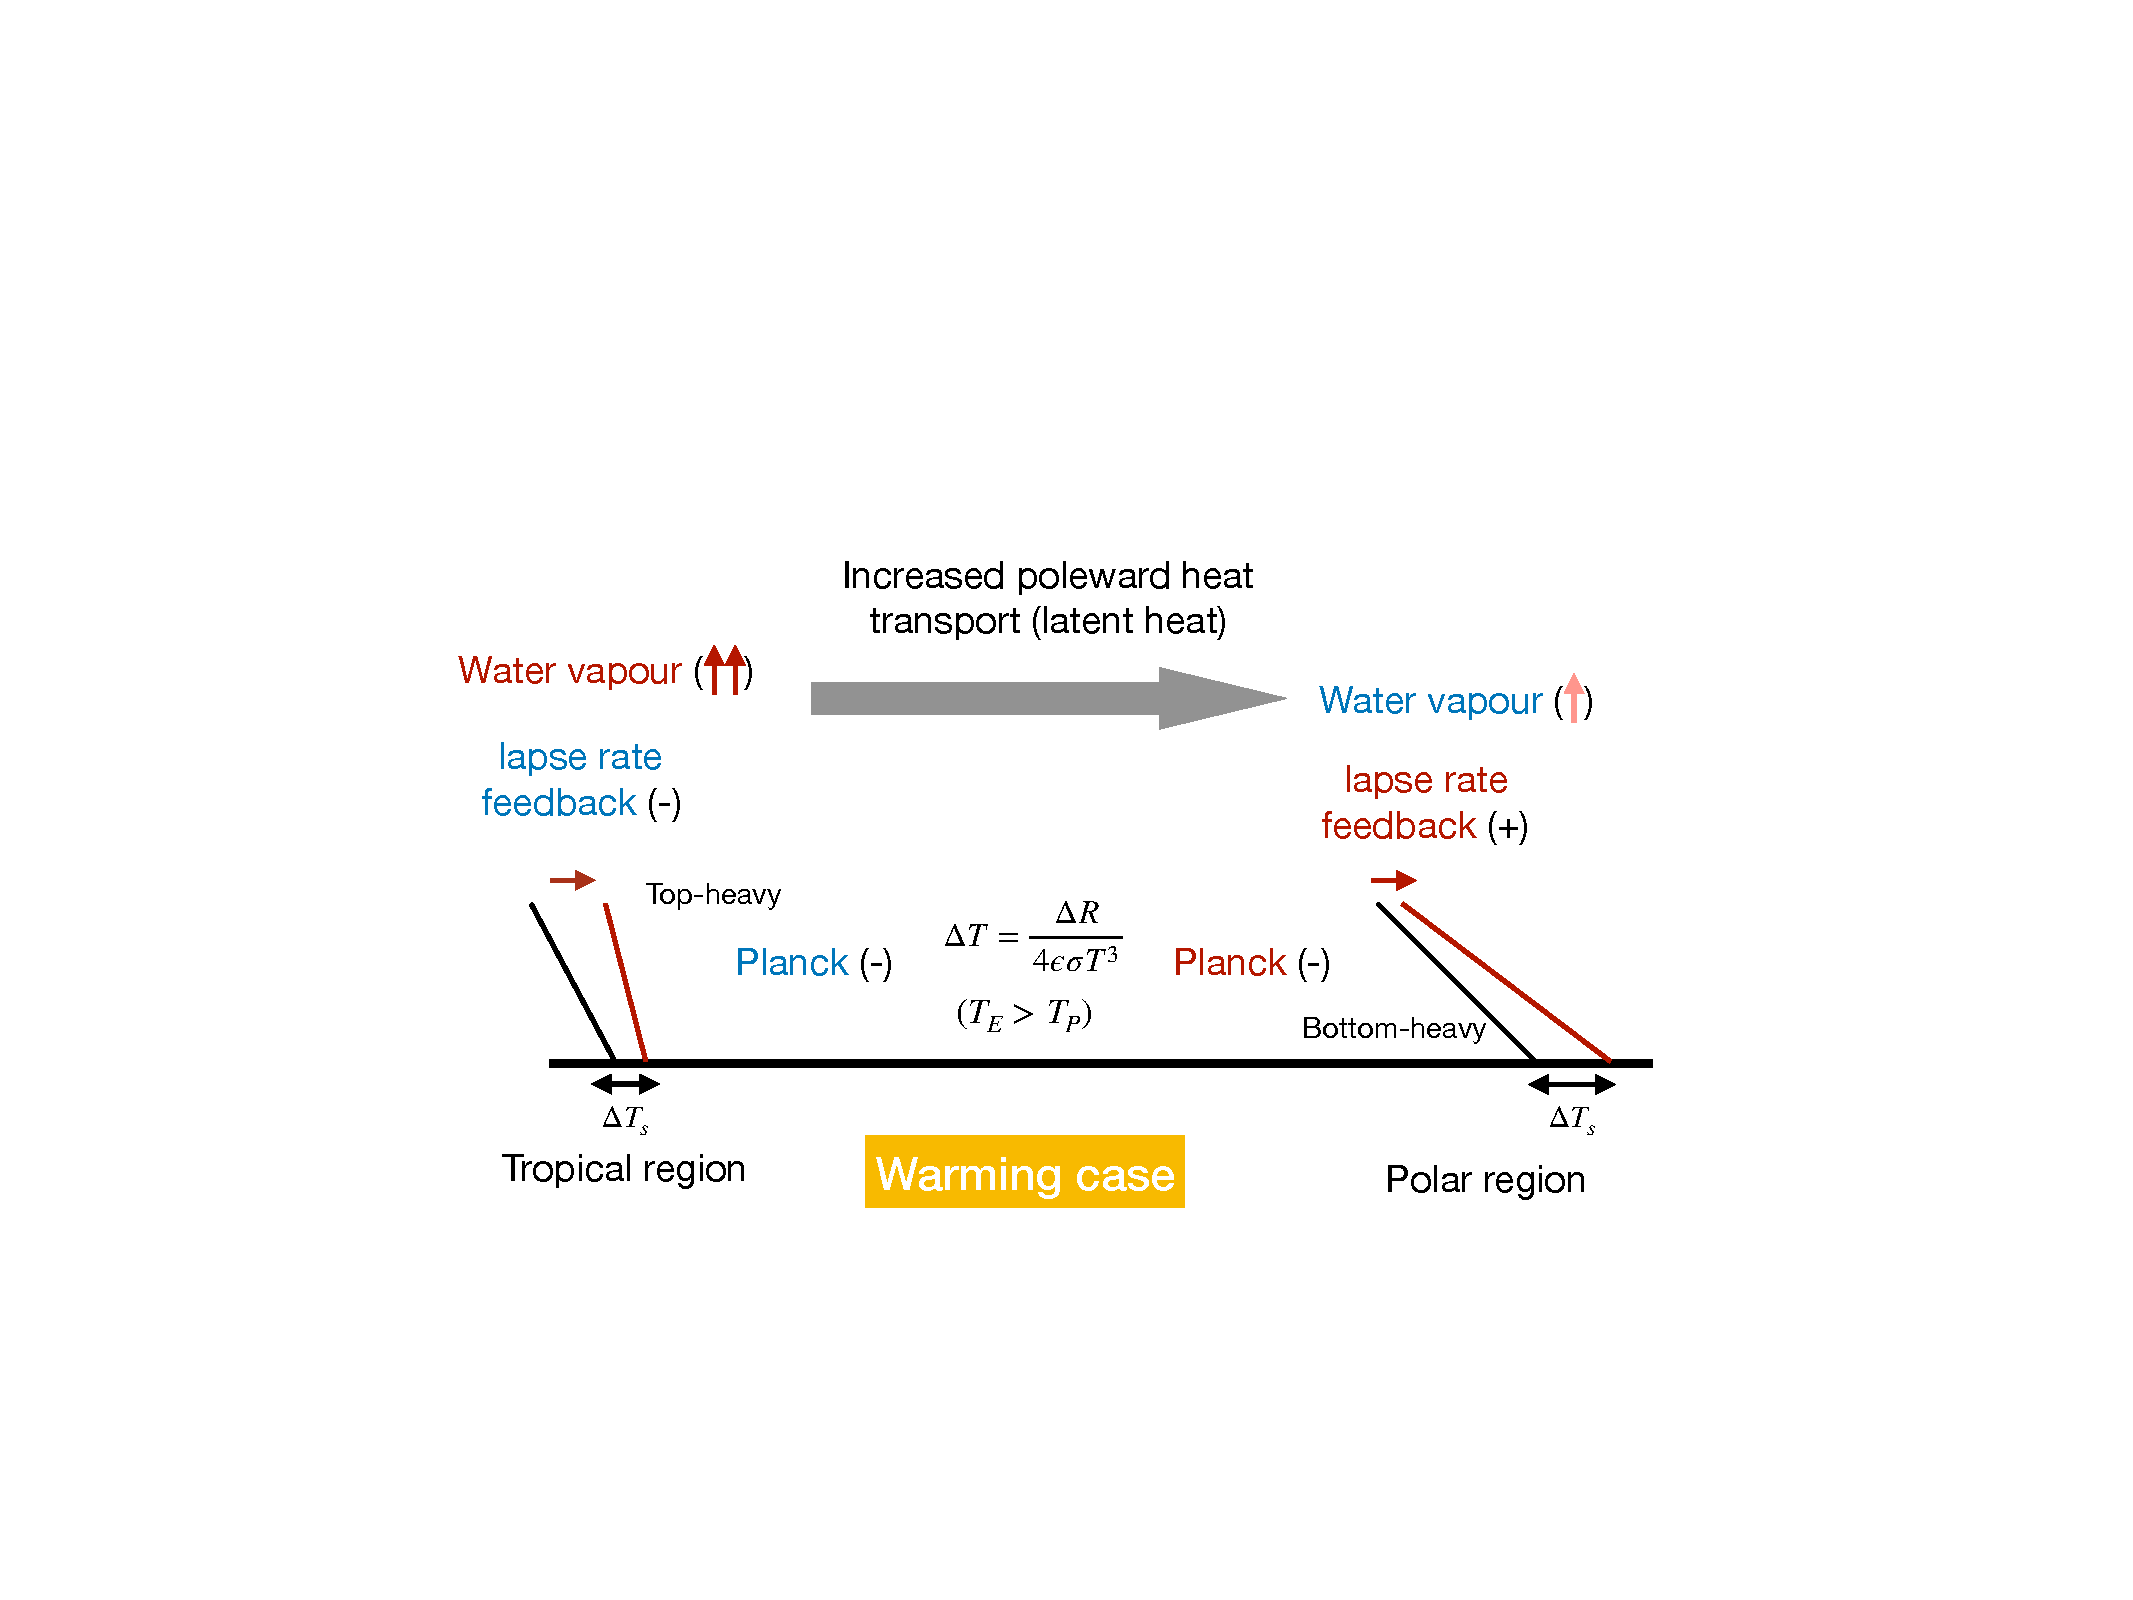
\includegraphics[width=0.8\textwidth]{figs/polar_amp/pa_dynamic.pdf}
	\caption{A schematic diagram to illustrate the various factors that contribute to the polar amplification.}
	\label{fig:pa_mechanism_schematic}
\end{figure}

The comparison of results from BOG and Frierson gives us some insights about the role of water vapor feedback in surface temperature change. After turning off the water vapor feedback in the BOG scheme, the surface temperature responses are much smaller and become close to the simulation results from Frierson scheme. However, there is still the amplified surface temperature change at high latitudes, which is associated with the poleward atmospheric energy transport. Following \cite{Feldl2013} and \cite{Kim2018}, the decomposition of the surface temperature change illustrates the relative importance of various contributions to surface temperature change at high latitudes. Specifically, heat transport, Planck feedback and the positive lapse rate feedback at polar region are all supportive to the polar amplification. However, water vapor feedback and the forcing induced by altering albedo contribute more to the surface temperature change at low latitudes than at high latitudes (\figref{fig:contribution_pole_vs_tropic}). In spite of that, the water vapor feedback is very strong at high latitudes in BOG scheme, which could explain the large temperature response in the experiments. A schematic of the mechanisms that contribute to the polar temperature changes is illustrated in \figref{fig:pa_mechanism_schematic}.

In summary, our findings have confirmed that polar amplification could exist even without sea ice and surface albedo feedback in aquaplanet simulations, which is consistent with the previous results \citep{Langen2007,Kim2018,Alexeev2005}. However, we have not explored the role of clouds in polar amplification, due to lack of cloud schemes in Isca model currently. As assessed by \cite{Kim2018}, the cloud radiative effects are negative in high latitudes due to an increase of low-level cloud amount and positive in low latitudes due to a decrease of overall cloud amount, which could explain in part why the polar amplification of surface temperature is large in our simulations. 

% But this will be studied in further chapters.

%Some studies also analyzed the effect of clouds radiative feedback to polar amplification \citep[e.g.][]{Kim2018}, where they found that polar clouds will have a cooling effect under global warming. Which could be
